\chapter{入出力と配列・シミュレーション}\label{chapter:io}
\begin{itembox}[l]{概要}
様々な解法につながる基本として,入力データを逐一調べる問題から始めて,配列と周辺の基本操作をとりあげる.
また,プログラムを一度に作成するのではなく,部品ごとに作ってテストするスタイルを身につける.
さらに,データの量に応じて,適切なアルゴリズムが必要になることを経験する.
\end{itembox}


\section{最大値,最小値}

\begin{psbox}{ICPC Score Totalizer Software}{国内予選2007}
入力として与えられる数値列から最大値と最小値を除いた平均値を求めよ.

入力はそれぞれが競技者の演技ひとつに対応するいくつかのデータセットからなる. 入力のデータセット数は20以下である.
データセットの最初の行はある演技の採点に当たった\uline{審判の数 n} ($3 \le n \le 100$) である.引き続く n 行には各審判のつけた \uline{点数 s} ($0 \le s \le 1000$) がひとつずつ入っている. n も各 sも整数である.入力中にはこれらの数を表すための数字以外の文字はない.\sout{審判名は秘匿されている.}
入力の終わりはゼロひとつの行で示される. 
  
\aojid{1147}
\end{psbox}


``Sample Input''を順に解釈すると,以下のように4つのデータセットからなることが分かる.
\begin{itemize}
\item (N=) 3 (S=) 1000 342 0
\item (N=) 5 (S=) 2 2 9 11 932 
\item (N=) 5 (S=) 300 1000 0 200 400
\item (N=) 8 (S=) 353 242 402 274 283 132 402 523
\item 0 (入力の終わり)
\end{itemize}

\begin{alltt}
#--------
3 # データは3つ, N=3
1000 # 最大値
342
0 # 最小値
#--------
5 # データは5つ, N=5
2 # 最小値
2
9
11
932 # 最大値
#--------
5 # データは5つ
300
1000 # 最大値
0 # 最小値
200
400
#--------
8 # データは8つ
353
242
402
274
283
132
402
523
#--------
0 # これでおしまい
\end{alltt}


同様に``Sample Ouput''を解釈すると,上記の各データセットに対して一つ数
値が出力されていることが分かる.
\begin{itemize}
\item 342 (そのまま)
\item 7 (2, 9, 11の平均)
\item 300 (300, 200, 400の平均)
\item 326 (...の平均)
\end{itemize}

\subsection{プログラム作成}

以下に,審判の得点の合計を計算するプログラムと最大得点を計算するプログラムを示す.(問題が求めるもの
は合計や最大値ではないので,これらは問題への直接の回答ではない).
必要ならばこれらのプログラムを参考に,問題への回答を作成せよ.

\begin{cbox}[emphstyle={[2]\graytext},emph={[2]iostream,using,namespace,std,cin,cout,endl}]
#include <iostream>
using namespace std;
int N, S;
int main() {
    while (cin >> N && N>0) {
        int sum = 0;
        for (int i=0; i<N; ++i) {
            cin >> S;
            sum += S; // std::accumulateを使っても良い
        }
        cout << sum << endl;
    }
}
\end{cbox}

\begin{cbox}[emphstyle={[2]\graytext},emph={[2]iostream,using,namespace,std,cin,cout,endl}]
// (一部略)
    while (cin >> N && N>0) {
        int largest = 0;
        for (int i=0; i<N; ++i) { // std::max\_elementを使っても良い
            cin >> S;
            if (largest < S) largest = S;
        }
        cout << largest << endl;
    }
\end{cbox}
C言語からC++に移行する場合は,(基本は共通なので)さしあたり\cplusplus{網掛け}部分を覚えて使えるようになると良い.
コンパイルの仕方などは\ref{section:commands}節を参照.

\begin{warningbox}{C言語禁止}
  本資料を読み進める場合は,C言語では不十分で,C++の機能の一部を使う必要がある.必要な部分を少しづつ紹介するので,この時点で\texttt{iostream,cin,cout}などに慣れること.
\end{warningbox}

\begin{tipsbox}{関数を使おう}
  \texttt{max,min,sum}などは関数を使っても良い.
\end{tipsbox}

\begin{pybox}
while True:
    N = int(input())
    if N == 0:
        break
    S = []
    for i in range(N):
        S.append(int(input()))
    print(sum(S))
    print(max(S))
\end{pybox}
なお,Python3で整数除算を行うには\texttt{/}に代えて\texttt{//}という演算子を用いる.


\subsection{動作テスト}

\subsubsection{サンプル入力を用いたテスト}

問題文中の``Sample Input''に対する出力が合うことを確認してみよう.

\subsubsection{審判データを用いたテスト}
この問題は審判が用いた秘密の入出力が公開されている.これを利用し
て, プログラムの誤りの有無をさらに手元で試験することができる.
(プログラムが``Sample Input'' には正しく振舞うが,他のデータには誤ることを発見できるかもしれない)
\begin{itemize}
\item 入力 \url{http://www.logos.ic.i.u-tokyo.ac.jp/icpc2007/jp/domestic/datasets/A/A1}
\item 出力 \url{http://www.logos.ic.i.u-tokyo.ac.jp/icpc2007/jp/domestic/datasets/A/A1.ans}
\end{itemize}

出力の一致を確認するには,\texttt{diff}コマンドを用いる.
実行方法などは\ref{section:commands}節を参照.

\begin{terminal}
$ python3 icpc.py < A1 > my-out.txt
$ diff -u my-out.txt A1.ans  
\end{terminal}

\begin{terminal}
$ ./a.out < A1 > my-out.txt
$ diff -u my-out.txt A1.ans  
\end{terminal}

\begin{warningbox}{後回し禁止}
  この時点で(次の章に進む前に)リダイレクションと\texttt{diff}の操作を覚えること.
\end{warningbox}


\section{計算時間の見積と試行回数}

コンピュータが得意な解法は全部を力づくで試すことである.実際に多くの問題をそれで解くことが出来る.
コンピュータが得意な解法は全ての可能性を力づくで試すことである.実際に多くの問
題をそれで解くことが出来る.
全ての可能性を列挙するには,for文を用いたり,再帰を用いたりする.

\begin{pbox}{Tax Rate Changed}{国内予選2014}
2つの商品の消費税率変更前の税込合計価格を元に, 新消費税率での税込合計
価格が最大いくらになるかを計算するプログラムを作って欲しい. 1円未満切り捨て等の細かい条件は問題文を参照のこと. 

制約(抜粋): $10 < s < 1000$, 商品の税抜価格は$1$円から$s-1$円のすべてを考慮に入れる

Time Limit : 8 sec, Memory Limit : 65536 KB

\aojid{1192}
\end{pbox}

 (1) 2つの商品の価格の候補の組み合わせを全通り試す.(2) 候補が,変更前
の税率で合計価格になっているかを調べる.そうでなければ捨てる (3) 変更
後の税率での合計価格を計算する.最大値なら記憶する.
という方針で作ってみよう.

仮に税込みの価格を計算する\texttt{tax(rate, price\_without\_tax)}という関数があっ
たとすると,次のような構造になるだろう.問題文では小文字の$s$を使って
いるが,本資料のプログラムでは(i, j, kなどの変数と区別して問題文由来である目印に)大文字で表記する.
\begin{cbox}
  int maximum = 0;
  for (int i=1; i<S; ++i)
    for (int j=i; j<S; ++j) 
      if (tax(X,i)+tax(X,j) == S) // (*)
        maximum = max(maximum, tax(Y,i)+tax(Y,j));
\end{cbox}
なおこの例題はさらに,繰り返し回数を減らすための工夫を検討することもで
きるが,C++なら今回は必須ではない.
Pythonの場合は,多少の工夫が必要である.下記のコードでは,ある組$(a_0,b_0)$の税込価格が$S$を越えたら,$b>b_0$での組$(a_0,b)$の税込価格も$S$を必ず超えるので,検討不要であるという性質を利用した.

\begin{warningbox}{関数必須 (横着禁止)}
  必ず関数 \texttt{tax}を作成すること.徐々に複雑なプログラムを扱う際に,関数の作成能力は重要となる.この時点で身につける.
\end{warningbox}

\begin{pybox}[emph={break}]
def tax(p,x):
    return p*(100+x) // 100     # 整数除算
def solve(X,Y,S):
    for a in range(1,S):
        for b in range(1,S):
            sum = tax(a,X)+tax(b,X)
            if sum == S:
                # 新税でのtax(a,Y)+tax(b,Y) について検討
            if sum > S:
                break           # b増加ならばsum増加のため
    return best
while True:
    X,Y,S = map(int, input().strip().split(' '))
    if X == 0:
        break
    print(solve(X,Y,S))
\end{pybox}

\begin{debugbox}{TLE (Time limit exceeded)}
  Pythonの場合はC++よりも実行速度が遅くなるため,C++と同じ方針ではACを
  得られない場合がある.例えば,上記のサンプルコードでは9,10行目に高速化のための工夫を施している.
\end{debugbox}

\begin{warningbox}{税込み v.s. 税抜き}
  本資料では,税抜価格と税率から税込価格を求める関数を作成した.向きを反対にして,税込み価格から税抜価格を求めるアプローチはどうだろうか.実はそちら向きは罠が多数あるのでお勧めしない(興味がある場合はお勧めの方法でAC後に理由を考えてみよう).
\end{warningbox}

\paragraph{複数データセットの入力}
この問題ではデータセットが複数与えられうる.すなわち,データが与えられ
る間はそれを読み込んで解を出力し,データが終了したらプログラムを終了さ
せる必要がある.「入力の終わりは,空白で区切られた3つのゼロからなる行
によって示される. 」という条件と通常のデータセットでは\texttt{X}が正であることを活用し,以下の構造でプログラムを書くことを勧める.

\begin{cbox}
#include <iostream>
using namespace std;
int X, Y, S;
int solve() {
  ... // X,Y,Sについて,最大値を計算
}
int main() {
    while (cin >> X >> Y >> S && X>0) {
	cout << solve() << endl;
    }
}  
\end{cbox}

\texttt{while}文の条件の\texttt{cin >> X >> Y >> S}の部分は\text{cin}への参照を
返し,\texttt{bool}にキャストされた際に,\texttt{cin}が正常状態かどう
か,すなわち\texttt{X, Y, S}を正常に読み込めたかどうかを返す.入力ファイルが間違っていた(よくある場合は,タイプミスまたは違う問題の入力を与えた)場合はここが\texttt{false}になって終了する.読み込めた場合に,\texttt{X, Y, S}は処理すべきデータセットの\texttt{X, Y, S}を読んだ場合と,入力終了の目印の空白で区切られた3つのゼロを読んだ場合の両方がある.前者の場合は正の整数であるはずなので,0かどうかをテストして判別する.

\paragraph{AOJへの提出}

上記の方針でプログラムを作成し,AOJでacceptされることを確認せよ.

もしacceptが得られなかった場合は手元での検証が可能である.まず,入力
(\url{http://icpc.iisf.or.jp/past-icpc/domestic2014/qualify14_ans/A1})
と正答
(\url{http://icpc.iisf.or.jp/past-icpc/domestic2014/qualify14_ans/A1.ans})
をダウンロードしておく.
\begin{terminal}
  $ ./a.out < A1 > my-output.txt
  $ diff -u A1.ans my-output.txt 
\end{terminal}
差があれば行数が表示される.

\paragraph{計算量の簡単な検討 (estimation of the number of trials)}
多くのコンテストの問題では実行時間に制限がついているので,実行
時間を見積もり間に合う解法を考案することが必要な場合もある.またコンテ
ストを離れて実用に用いるプログラムでも,何らかの実行速度に関する要請が
ある場合が多い.プログラムを書き終えてから速度に問題があることが分かる
と,書き直しが困難な場合もあるので,プログラムを書く*前*に何らかの見通
しを得ておくことが望ましい.

現実の計算機は複雑な装置であるから,正確な実行時間の予想は簡単ではない.よって単純なモデルに基づく目安を考える.
たとえば,プログラムを実行する過程で,加減乗除のような基本演算が何回行
われるかを数える.このモデルでは加算と除算では速度が異なりうるとか,同時に
二つの命令を実行される場合があるなどの,細かい点は無視している.目安で
あるので現実との対応関係は別に議論が必要だが,役に立つ場面も多い.


上記のプログラムで4行目(*)が最大何回実行されるか,考察しよう(厳密に求めなくて良い).
回数を($S$に依存するので),$f(S)$と表すとする.2行目の\texttt{for}ループ
が$S$回,3行目の\texttt{for}ループが最大$S$回繰り返すので,$f(S) \le
S^2 \le 1\,000^2=10^6$である.

\begin{table}[h]
  \centering
  \caption{\cemphp{C++}で,1秒間で実行可能な演算回数の目安 (\cite{book:pcc}を改変して転載)}
  \label{table:empirical-estimation}
  \begin{tabular}{rl}\hline
    $1\,000\,000$  &余裕を持って可能\\
    $10\,000\,000$ &たぶん可能\\
    $100\,000\,000$&とてもシンプルな演算なら可能\\\hline
  \end{tabular}
\end{table}

この回数($10^6$)を表\ref{table:empirical-estimation}に当てはめると,(tax関数が効率的に実装されていることを前提に)余裕を持っ
て,1秒間で実行可能と分かる.\footnote{注: この見積もりは1つのデータセットについてのものである.一方,問題全体では「入力は複数のデータセットからなる」ものを8秒間で回答する必要があるため,計算時間はデータセット数の上限を考慮して見積もる必要がある.データセットの数について記述がない場合は,厳密には問題の不備であるが,10個程度と考えて良い.}
表の数値は,実行環境に合わせて経験的に測定する必要がある.
目安として,最近の多くのコンピュータのCPUは1GHz ($=10^{9}$)程度で動作しているので,CPUが100サイクル以内に実行できる演算なら,1秒間に$10^6$回実行可能と期待できる.

本資料の範囲では,この表を信じて問題ない場合がほとんどであるが,
正確な予測のためには,キャリブレーションを行う.すなわち,作成した解法が入力に対応する数値$N$に関しておよそ何回の基本演算を行う
かを見積もったら,いくつかの$N$に対応する入力で実験し,実際の計算秒数
との対応を取る.たとえばメモリ参照やnew/deleteは,算術演算よりそれぞれ10倍,100倍以上に遅い場合がある.また,C, C++以外の言語では,実行により時間がかかることも多い.問題ごとの秒数制限と,オンラインジャッジのハードウェアを考慮して検討する.

\begin{tipsbox}{Pythonの場合はC++よりも実行速度が遅くなる}
  問題によるが20-200倍余裕
  をもって見積もると良い.オンラインジャッジで時間制限は
  Pythonに適切とは限らないので,ジャッジデータをダウンロードして正答を確認できればそれでも良い.
\end{tipsbox}


\begin{pbox}{Space Coconut Grab}{模擬国内予選2007}
宇宙ヤシガニの出現場所を探す.エネルギーEが観測されたとして,
出現場所の候補は,$x+y^2+z^3=E$を満たす整数座標(x,y,z)で,さらにx+y+zの
値が最小の場所に限られるという.x+y+zの最小値を求めよ.
(x,y,zは非負の整数,Eは正の整数で1,000,000以下,宇宙ヤシガニは,宇宙最大とされる甲殻類であり,成長後の体長は 400 メートル以上,足を広げれば 1,000 メートル以上)

\aojid{2012}
\end{pbox}

まず,全部試して間に合うかを考える.
(間に合うならそれが一番実装が簡単なプログラムである)

変数x,y,zの動く範囲を考えると,それぞれx:[0,E], y:[0,$\sqrt{E}$],
z:[0,${}^3\sqrt{E}$]である.それら(x,y,z)の組み合わせは,Eの最大値は
1,000,000$=10^6$であるから,最大$10^6 \cdot 10^3 \cdot 10^2=10^{11}$で
ある.
制限時間が8秒であることを加味しても,この方針では間に合いそうにない.

減らす指針として,全ての(x,y,z)の組み合わせを考える必要はなく,
$x+y^2+z^3=E$を満たす範囲だけで良いことを用いる.たとえば,xとyを決める
と,Eからzは計算できる(zが整数とならない場合は無視して良い).この方針で
調べる種類は,(x,y)の組み合わせの種類である,$10^6 \cdot 10^3$となる.
この値はまだ大きいが,先ほどと比べると1/100に削減できている.上記と同様
に,xとzを決めてyを求める,z,yを決めてxを求めることもできる.それらの方
針の場合に,調べる組み合わせの種類を求めよ.一番少ないものが間に合う範
囲であることを確認し,実際に実装してAOJに提出して確かめる.

\begin{debugbox}{Python--TLE}
残念ながら上記の方針ではPythonでは時間制限を超過(TLE)する.対策として
は,2重ループを避けて\texttt{z}に関する1重ループのみにすれば良い.
単調性から\texttt{y}に関するループを省くことが出来る.
\begin{pybox}
import math
# ...(中略)...
y = int(math.floor(math.sqrt(E-z**3)+1e-7))
\end{pybox}
\end{debugbox}

\section{練習問題}
\begin{pbox}{Square Route}{模擬国内予選2007}
縦横1500本程度の道路がある街で,正方形の数を数えてほしい.

\aojid{2015}
\end{pbox}

注: 全ての4点を列挙して正方形になっているかどうかを試すと間に合わないので,工夫した方法が必要である.正方形を一つづつ数えると数が多すぎるので,一定の性質を持つ正方形をまとめて数えるような方法が必要となる.

ヒント: 後の章で扱う標準データ構造を活用する方法と,正方形の初等的な性質を利用する方法がある(\textcolor{white}{対角線を延長した直線を共通に持つ正方形}について考えてみよう).


\chapter{整列と貪欲法}\label{chapter:greedy}

\begin{itembox}[l]{概要}
ある基準に従ってデータを並べ替えることを整列(sort)という.
ほとんどの言語の標準ライブラリでは,整列の方法が提供されているので,ま
ずはそれの使い方を習得しよう.この資料では整列された結果
を得られれば良いという立場をとるが,整列の手法そのものに興味がある場合は,たとえ
ば~\pcaojbook[pp.~51--(3章)]を参照されたい.

データの整列は,問題解決の道具として活躍する場合もある.それらには,最適化問題や配置問題など,整列とは関係がない見た目の問題も含まれる.
\end{itembox}

\section{さまざまな整列}

\subsection{数値の整列}\label{section:sort}

C++とRubyでは,標準関数として\texttt{sort}や\texttt{sort!}が用意されている.
\begin{cbox}[emph={algorithm,sort}]
#include <algorithm>
#include <iostream>
using namespace std;
int A[5] = {3,5,1,2,4};
int main() {
   sort(A,A+5); // 半開区間[l,r)で指定する.sort(\&A[0], \&A[5])と同じ意味
   ... // coutにAを出力してみよう
}
\end{cbox}
配列を整列させる範囲を指定するには,\texttt{\&A[0]}のように配列の要素を指すポインタを用いる.一次元配列の場合に単に\texttt{A}と書けば,先頭要素を指すポインタに自動的に変換される.
配列でなく\texttt{vector}や\texttt{array}の範囲を指定するには,
\texttt{A.begin(),A.end()}という表記を用いる.この\texttt{begin}や\texttt{end}はポインタを一般化したイテレータを返す関数で,名前の通りの場所を指し示す.他に\texttt{A.begin()+2,A.begin()+5}のように一部の区間を指定することもできる.さらにC++11以降では\texttt{begin(A)}とすることで配列もvectorも共通に扱うことができる.

\begin{pybox}[emph=sort]
a = [3,5,1,2,4]
a.sort()
a
# [1, 2, 3, 4, 5]  
\end{pybox}


\begin{psbox}{Sort II}{AOJ}
 与えられたn個の数字を昇順に並び替えて出力するプログラムを作成せよ. 

\aojid{10029}
\end{psbox}

回答例:
\begin{cbox}
int N, A[1000000+10];
int main() {
    cin >> N;
    for (int i=0; i<N; ++i) cin >> A[i]; // Aの入力
    ... // Aをソートする
    for (int i=0; i<N; ++i) cout << (i?" ":"") << A[i]; // Aの出力
    cout << endl;
}
\end{cbox}

出力部分の\texttt{(i?" ":"")}は,要素の間にのみ空白文字を入れるための微調整(先頭\texttt{i==0}には空白を入れない).

\subsection{文字列の整列}

\begin{psbox}{Finding Minimum String}{AOJ}
N個の小文字のアルファベットのみからなる文字列の,辞書順で先頭の文字列
を求める.
問題文中に記述がないがNは1000を越えない.

\aojid{10021}
\end{psbox}

補足: 辞書式順序は,大文字小文字が混ざる場合はC++の\texttt{std::string}の比較演算子の比較順序とは異なる.(が,今回は小文字のみなのでその心配はない)

\begin{cbox}
#include <algorithm> // sortのため
#include <string> // string (文字列)のため
#include <iostream>
using namespace std;
string A[1000];
int N;
int main() {
    cin >> N;
    if (N > 1000) abort();
    for (int i=0; i<N; ++i) cin >> A[i];
    ... // 整数の時と同様にAを整列(sort)する
    cout << A[0] << endl;
}
\end{cbox}

\subsection{ペアと整列}\label{section:sort-pairs}
\subsubsection{ペア}
ペア(組み)の表現を導入する.$\langle$開始時刻,終了時刻$\rangle$や$\langle$身長,体重$\rangle$,$\langle$学籍番号,点数$\rangle$など,現実世界の情報にはペアとして表現することが自然なものも多い.

\begin{cbox}
#include <utility> // pairのため
#include <iostream>
using namespace std;
int main() {
  pair<int,int> a(2,4); // 整数のペア
  cout << a.first << ' ' << a.second << endl; // 2 4と表示

  a.first = 3;
  a.second = 5;
  cout << a.first << ' ' << a.second << endl; // 3 5と表示

  a = make_pair(10, -30);
  cout << a.first << ' ' << a.second << endl; // 10 -30と表示

  pair<double,char> b; // 小数と文字のペア
  b.first = 0.5;
  b.second = 'X';
  cout << b.first << ' ' << b.second << endl; // 0.5 Xと表示
}
\end{cbox}

Pythonやruby の場合は列(配列やリスト)を手軽に使えるので,(取り立ててpairを区別せず)列を使う.



\subsubsection{ペアの配列と整列}
続いて,ペアの配列を扱う.たとえば,一人の身長と体重をペアで表現する時に,複数の人の身長と体重のデータはペアの配列と対応づけることができる.
前回,整数の配列を整列(\texttt{sort})したように,ペアの配列も整列することができる.
標準では,第一要素が異なれば第一要素で順序が決まり,第一要素が同じ時には第二要素が比較される.

\begin{cbox}
#include <utility> // pairのため
#include <algorithm> // sortのため
#include <iostream>
using namespace std;
int main() {
  pair<int,int> a[3]; // 整数のペア
  a[0] = make_pair(170,60);
  a[1] = make_pair(180,90);
  a[2] = make_pair(170,65);

  for (int i=0; i<3; ++i) // a[0]からa[2]まで表示
    cout << a[i].first << ' ' << a[i].second << endl;
  // 170 60
  // 180 90
  // 170 65 と表示されるはず

  sort(a, a+3); // a[0]からa[2]まで整列

  for (int i=0; i<3; ++i) // a[0]からa[2]まで表示
    cout << a[i].first << ' ' << a[i].second << endl;
  // 170 60
  // 170 65
  // 180 90 と表示されるはず
}
\end{cbox}

\begin{pybox}
a = [[3,5],[2,9],[3,6]]
print(a) # [[3, 5], [2, 9], [3, 6]]
a.sort()
print(a) # [[2, 9], [3, 5], [3, 6]]
\end{pybox}

\subsubsection{3つ以上の組}
C++11では,3つ以上の組を表す\texttt{tuple}型が用意されている.\footnote{\url{http://en.cppreference.com/w/cpp/utility/tuple}}
それより前のC++では\texttt{pair<int,pair<int,int> >}などと\texttt{pair}を重ねて用いていたところが,簡潔に書けるようになった.

\begin{c11box}[emph={tuple}]
#include <tuple>
#include <iostream>
#include <algorithm>
using namespace std;
int main() {
  tuple<int,int,int> a = {3,1,4};
  cout << get<0>(a) << "\n";	// 3
  cout << get<1>(a) << "\n";	// 1
  cout << get<2>(a) << "\n";	// 4

  tuple<int,int,int> array[] = {{3,1,4}, {1,5,9}, {2,6,5}};
  sort(array, array+3);
  
  tuple<int,int,int> t = array[0];
  cout << get<0>(t) << "\n";	// 1
  cout << get<1>(t) << "\n";	// 5
  cout << get<2>(t) << "\n";	// 9
}
\end{c11box}


\subsection{大きい順に整列}
標準の\texttt{sort}関数は小さい順に並べ替える.大きい順に並べ替えるに
はどのようにすれば良いだろうか?
\begin{enumerate}
\item 小さい順に並べ替えた後に,並び順を逆転させる (当面これで十分)
\begin{cbox}
int A[5] = {3,5,1,2,4};
int main() {
   sort(A,A+5);
   // C++11なら sort(begin(A),end(A));
   reverse(A,A+5); // 与えられた範囲を逆順に並び替え
   ...  // coutにAを出力してみよう
}
\end{cbox}
\begin{pybox}
a = [3,5,1,2,4]
a.sort()
a.reverse() # aを逆順に並び替え
\end{pybox}
\item \texttt{reverse\_iterator}を使う
\begin{c14box}[emph={rbegin,rend}]
  sort(rbegin(A),rend(A));
\end{c14box}
\begin{pybox}
a.sort(reverse=True) 
\end{pybox}
\item 比較関数を渡す (汎用的)
\begin{c11box}
int A[5] = {3,5,1,2,4};
int main() {
   sort(begin(A),end(A),[](int p, int q){ return p > q; });
   ...  // coutにA[i]を出力してみよう
}
\end{c11box}
文法の説明は省略するが\texttt{[](int p, int q)\{ return p > q; \}}の部分が2つの整数の並び順を判定する匿名関数である.
\begin{pybox}
a.sort(key=lambda e: -e)  
\end{pybox}
\end{enumerate}

\section{貪欲法}

\subsection{良い順に使う}
\begin{pbox}{カントリーロード}{UTPC 2008}
カントリーロードと呼ばれるまっすぐな道に沿って, 家がまばら
に建っている. 指定された数までの発電機と電線を使って全ての家に給電したい. 
家に電気が供給されるにはどれかの発電機に電線を介してつな
がっていなければならず, 電線には長さに比例するコストが発生する. できるだけ電線の長さの総計が短くなるような発電機 お
よび電線の配置を求める.

\aojid{2104}
\end{pbox}

ヒント: 発電機が一つなら,端から端まで全ての家を電線でつなぐ必要がある.
発電機が2つなら,端から端まで全ての家を電線でつないだ状態から,家と家
の間の一箇所に電線を引かずに節約することができる.つまり,一番長い一箇所を節約するのが得.
発電機が3つなら,端から端まで全ての家を電線でつないだ状態から,家と家
の間で一番長い部分と二番目に長い部分には電線を引かずに節約することができる....

\begin{tipsbox}{方針の確認}
プログラムを書く前にSample Inputを手で解いてみよう
\end{tipsbox}


回答例
\begin{cbox}
int T, N, K, X[100000+10], A[100000+10];
int main() {
    cin >> T; // データセットの数を読み込む
    for (int t=0; t<T; ++t) {
        ... // 家と発電機の数を読み込む
        for (int i=0; i<N; ++i) cin >> X[i]; // 家の位置を入力
        for (int i=0; i+1<N; ++i) A[i] = X[i+1]-X[i]; // 家と家の間
        ... // 配列Aを整列する
        ... // 配列Aの先頭max(0,N-1-(K-1))個の和を出力する
    }
}
\end{cbox}

Python3の入力例: 与えられた1行を配列として読み込む場合は\texttt{list(...)}で変換する
\begin{pybox}
N,K = map(int,input().strip().split(' '))
X = list(map(int,input().strip().split(' ')) # リストへの変換を明示
\end{pybox}

\begin{debugbox}{よくある考え漏れ}
発電機\textcolor{white}{の個数が家の数を越えて増えても}節約できる区間は増えない (ヒントが白い文字で書かれているので,読みたくなったらコピーペーストなどで読むと良い).
\end{debugbox}

このような解法が貪欲法(greedy)と呼ばれる意味は,節約する区間の「組み合わせ」を
考えることなく,(長さ順に並べた)単独の区間を順に一つづつ見て閾値を越えるまで節約することを貪欲に決める点である.

\begin{pbox}{Stripies}{Northeastern Europe 2001}
質量が$m_1,m_2$である2体合体すると,$2\sqrt{m_1\cdot m_2}$となる種族がある.
初期状態を与えられるので,全てが合体した時の最小の質量を求めよ.

\url{http://poj.org/problem?id=1862}
\end{pbox}

小数点以下3桁を出力するには\texttt{printf("\%.3f\textbackslash{}n", ret);}を用いる.

\begin{pbox}{Princess's Marriage}{模擬国内予選2008}
護衛を上手に雇って,道中に襲われる人数の期待値を最小化する.
護衛は1単位距離あたり1の金額で,予算がある限り,自由に雇える.

入力は,区間の数N, 予算Mに続いて,距離と1単位距離あたりの襲撃回数の期
待値のペア$\langle$D,P$\rangle$がN個.  


\aojid{2019}
\end{pbox}

考え方:
せっかく護衛を雇うなら,もっとも危険な区間を守ってもらうのが良い.
一番危険な道を選び,予算がある限りそこに護衛を雇う.予算の残額で道の区間全てをカバーできない場合は,安全になる区間と,危険なままの区間に道が分かれる.予算が残っている限り,2番目に危険な道,3番目に危険な道の順に同様に繰り返す.残った危険な区間について,期待値の和が答えとなる.
この計算課程では,$\langle$危険度,長さ$\rangle$のペアで道を表現し,危険な順に整列しておくと便利である.  (ここで危険度は,距離1移動する間に襲われる回数の期待値を表す)

回答例 (入力と整列):
\begin{cbox}
int N, M;
pair<int,int> PD[10010];
int main() {
  while (cin >> N >> M && N) {
    int d, p;
    for (int i=0; i<N; ++i) {
      cin >> d >> p;
      PD[i] = make_pair(p, d);
      // PD[i].first は道iの危険度
      // PD[i].second は道iの長さ
    }
    ... // PDを大きい順に整列しよう
    // 整列がうまく行ったか,PDを表示してみよう
    // うまく整列できたら,次は答えを計算しよう
  }
}
\end{cbox}

回答例 (答えの計算):
\begin{cbox}
    int S = 0;
    for (int i=0; i<N; ++i)
      S += 道[i]の危険度 * 道[i]の長さ;
    // 予算0の時の答えが,現在のSの値
    for (int i=0; i<N; ++i) {
      if (M <= 0) break;
      int guarded = Mと道[i]の長さの小さい方; // 雇う区間
      S -= 道[i]の危険度 * guarded;
      M -= guarded;
    }
    S が答え
\end{cbox}

\begin{itemize}
\item 予算が0の場合は,答えとして必要な ``刺客に襲われる回数の期待値''である $S$は,各道$i$について$S=\sum_i P_i\cdot{}D_i$となる.
\item 予算がMの場合,$S$から護衛を雇えた区間だけ期待値を減らす.例えば
  道$j$の区間全部で護衛を雇うなら $P_j\cdot{}D_j$だけ$S$を減らすことができる.もし残り予算$m$が道の長さ$D_j$より小さく道の一部だけしか護衛を雇えないなら$S$から減らせるのは$P_j\cdot{}m$だけである.
\end{itemize}

\subsection{区間スケジューリング}

「アルゴリズムデザイン」\cite{book:algorithmdesign}の4.1章(pp.~104--108)を参照.

\paragraph{問題概要}
一つの共有資源(体育館,駐車場など)と多数の利用申請(開始時刻と終了時刻
のペア)があったとする.使用時間が衝突しないように,利用申請の部分集合
を選ぶ.最大いくつの申請を採用できるか?

\centerline{\begin{tikzpicture}
\draw (3,3.5) -- node[above]{$$} (5,3.5) node[right]{$0$};
\draw (1,3) -- node[above]{$$} (3.5,3) node[right]{$1$};
\draw (6,2.5) -- node[above]{$$} (7,2.5) node[right]{$2$};
\draw (2,2) -- node[above]{$$} (4.5,2) node[right]{$3$};
\draw (1.5,1.5) -- node[above]{$$} (2.5,1.5) node[right]{$4$};
\draw (4,1) -- node[above]{$$} (7.5,1) node[right]{$5$};
\draw[color=gray,dotted,->] (0,0.5) -- (8,0.5) node[right] {time};
\end{tikzpicture}}

単純化: 体育館や時刻などの具体を削ぎ落とすと,線分の集合から一部を選択する問題になる.

\paragraph{直感と考察}

\begin{itemize}
\item 実は左から採用すれば良いのでは? \dingright{} そうでもない(反例有り)
\item 短い線分は他と重なりにくい.短い線分から採用すれば良いのでは? \dingright{} 必ずしもそうでもない(反例有り)
\end{itemize}

\paragraph{正しいアルゴリズム}

  \begin{enumerate}
  \item \cemph{右端が一番左にある線分}(i.e., 早く終わる申請)を選び,重なる線分とともに取り除く
  \item 未選択の線分がまだあれば,step.1に戻り手順を繰り返す
  \end{enumerate}


  
\paragraph{区間を扱う練習問題}

以下の問題は,区間スケジューリング問題とは異なるが,区間を扱う問題である.

\begin{pbox}{Cleaning Shifts}{USACO 2004 December Silver}
連続するT日の掃除当番を決めたい.各「牛」は何日目から何日目まで(境界を含む)区間働けることがわかっている.当番が不在の日の内容に牛を配置するとき,最低何頭必要か答えよ.不可能な場合は-1を出力せよ.

\url{http://poj.org/problem?id=2376}
\end{pbox}

ヒント: 当番に穴を空けない中で,もっとも遅くまで担当できる牛を採用してゆく.

\begin{tikzpicture}
\draw (1,2.5) -- (8,2.5);
\draw[color=ired] (1.5,2) -- (10,2) node[right] {best};
\draw (2,1.5) -- (5,1.5);
\draw (2.5,1) -- (7,1);
\draw[color=icyan] (3.2,0) -- (3.2,3) node[right] {$t$};
\draw[color=gray,->] (0,0.5) -- (14,0.5) node[right] {day};
\end{tikzpicture}


回答例 (入出力)
\begin{cbox}
int /*牛の総数*/N, /*掃除日数*/T;
pair<int,int> C[25010]; // C[i].firstが担当開始日,C[i].secondが担当終了日
int solve() {
  // N,T,Cを元に回答を計算する
}
int main() {
    scanf("
    for (int i=0; i<N; ++i)
      scanf("
    printf("
}
\end{cbox}

回答例 (計算)
\begin{cbox}
int solve() {
    sort(C, C+N); // 掃除開始日の早い順に整列
    int /*牛番号*/i = 0, /*次の担当の掃除開始日*/t = 1, /*採用数*/c = 0;
    while (i<N && t<=T) {
        int best = 0; // 次の雇う予定の牛の担当終了日
        while (i<N && 牛iの担当開始がtより遅くならない間) {
            ... // 牛iの担当終了がbestより遅ければbestを更新
            ++i;
        }
        if (担当可能な牛が一頭も居なければ(best<t)) return -1;
        t = best+1;
        ++c;
    }
    return /*Tまで掃除終了しているか?*/ ? c : -1;
}
\end{cbox}

戦略: $t-1$日目まで掃除が終わっていたとする.$t$日目を含む区間に掃除をできる牛がいなければ,解はない(-1を出力).もし複数の牛がt日目を担当可能であれば,なるべく長く担当してもらえる牛を雇うのが良い(*).その牛が$s$日まで担当したとすると,$t=s+1$として,全体の区間が終わるまで,牛を雇い続ける.

他の牛を雇っても最適解になる可能性はあるが,(*)の戦略をとった場合と比べて,雇う牛の数を減らすことはできないことが証明できる.


\begin{pbox}{Radar Installation}{Beijing 2002}
全ての島が見えるようにレーダーを配置する

注意: y=0の島が存在する模様

\url{http://acm.pku.edu.cn/JudgeOnline/problem?id=1328}
\end{pbox}


ヒント: 
\begin{itemize}
\setlength{\itemsep}{0pt}
\item 島が観測できるレーダーの区間を列挙したとする.まだレーダにカバーされていない島を一番沢山カバーできる場所にレーダを配置し,それを繰り返すという戦略を考える.この戦略が最適な配置より多くのレーダを必要とするような島の並びの例を示せ
\item 左から順にレーダを配置するとする.(まだレーダにカバーされていないなかで)見えはじめるのが最も左にあ
  る島を選び,その島が見える区間の左端にレーダを配置するとする.この戦略が最適な配置より多くのレーダを必要とするような島の並びの例を示せ
\item 左から順にレーダを配置するとする.(まだレーダにカバーされていないなかで)見えはじめるのが最も左にあ
  る島を選び,その島が見える区間の右端にレーダを配置するとする.この戦
  略が最適な配置より多くのレーダを必要とするような島の並びの例を示せ
\item 左から順にレーダを配置する正しい戦略Aを示し,他のどのような配置も戦略Aによる配置よりレーダ数が小さくならないことを証明せよ
\end{itemize}

\begin{debugbox}{よくあるバグ}
遠すぎる島など,例外を考慮する必要がある.複数のテストケースを扱うので,遠すぎる島があっても入力は全ての島を読み込むこと(さもないと次のテストケースで先頭がずれる).
\end{debugbox}

\subsection{様々な問題}

\begin{pbox}{Make Purse Light}{模擬国内予選 2005}
財布の中身を軽くする
  
\aojid{2007}
\end{pbox}

\begin{pbox}{Fox and Card Game}{Codeforces 388 C}
先手は山の一番上からカードをとり,後手は一番下から取る時,それぞれが最善を尽くした時の得点を求める.

\url{http://codeforces.com/problemset/problem/388/C}
\end{pbox}

\begin{pbox}{Shopping}{アジア大会2014}
  直線上に配置された複数の店を制約を満たしながら買い物をして左から右に抜ける時の,必要な移動の最小を求める.
  
  \aojid{1347}
\end{pbox}

\begin{pbox}{Dinner$\star$}{夏合宿2014}
食堂の食事と自炊を組み合わせてN日間の幸福度を最大化する.
  
  \aojid{2642}
\end{pbox}


\begin{pbox}{Ploughing$\star\star$}{13th Polish Olympiad in Informatics}
  畑を,縦(幅1列)か横(1行)にスパっと切りとることを繰り返して,区分けする.
どの範囲も数の合計がK以下になるようにする.条件を満たす最小の分割数を求めよ.

\url{https://szkopul.edu.pl/problemset/problem/6YiP6JA5U15hY94pLwuHoYPg/site/}
\end{pbox}

 \chapter{動的計画法 (1)}\label{chapter:dp}

\begin{tabular}{@{}cc@{}}
\begin{minipage}{.6\linewidth}
\begin{itembox}[l]{概要}
全ての可能性を調べ尽くすことが難しいような問題も,小さな問題を予め解いて解を表
に覚えておくなどの整理を適切に行うことで簡単に解けるようになる場合もある.
大小の問題の関係を表す式を立てて,それをプログラムにしてみよう.
動的計画法は,問題が持つ部分構造最適性を利用して効率の良い計算を実現する方法である.
\end{itembox}
\end{minipage}
&
\begin{minipage}{.35\linewidth}
\includegraphics[width=.45\linewidth]{DSC_0537s.JPG}
\includegraphics[width=.45\linewidth]{DSC_0541s.JPG}\\
\scriptsize フィボナッチ聖人の彫像\hfill(Camposanto, Pisa)
\end{minipage}

\end{tabular}


\section{数を数える}

\begin{psbox}{Fibonacci Number}{AOJ}
N番目のFibonacci数を求めよ。  

\url{http://judge.u-aizu.ac.jp/onlinejudge/description.jsp?id=ALDS1_10_A}
\end{psbox}

簡単のため$i$番目のFibonacci数を$F_i$と表記すると,以下のように定義される($F_0=0$と定義することも多いが本質ではないので問題文に合わせる):
\begin{equation}
  F_i = \left\{
  \begin{array}{ll}
    1 & i=0\\
    1 & i=1\\
    F_{i-1}+F_{i-2} & \mbox{(otherwise)}
  \end{array}\right.\label{eq:fib-recurrence}
\end{equation}

上記の定義をそのまま再帰で定義すると以下のようになるだろう:
\begin{pybox}
def fib(n):
    print("fib",n) # 関数呼び出しの際に引数を表示 (動作確認後に消す)
    if n == 0:
        return 0
    elif n == 1:
        return 1
    else:
        return fib(n-2)+fib(n-1)
\end{pybox}

しかし,この方法は計算の重複が多く,効率的でない.nの増加に伴い急速に遅くなる.
一例としてpythonの\tindex{timeit}モジュールを使った実行時間測定例を示す.
\begin{pybox}[emph=timeit]
import timeit
print(timeit.timeit("fib(10)", globals=globals(), number=10))
print(timeit.timeit("fib(20)", globals=globals(), number=10))
print(timeit.timeit("fib(30)", globals=globals(), number=10))
\end{pybox}

\begin{terminal}
$ python3 fib.py
0.0001415439764969051
0.01775405099033378
2.1516372300102375
\end{terminal}

今回主として扱う,より素直な方法は,小さいフィボナッチ数から順に計算す
ることである.
式(\ref{eq:fib-recurrence})から,$F_i$を求めるには,$F_0$から$F_{i-1}$までの値のみが必要であり,それらがあれば加算1回で計算できるという関係がわかる.そこで$F_0$から順に計算すれば,各$F_i$は加算1回で求められる.
\begin{cbox}
int F[100]; // 必要なだけ
int main() {
  F[0] = 1;
  F[1] = 1;
  for (int i=2; i<45; ++i) { // 必要なだけ
    F[i] = F[i-2]+F[i-1];
  }
}
\end{cbox}
この章で扱う問題は,求めたい問題の答え(e.g., $F_{100}$)が\jindex{部分問題}{ぶぶんもんだい}の答え($F_{n}, \; n<100$)から効率的に計算可能なものを取り扱う.
今回の場合は,回答にあたって直接必要なものは$N$番目のデータだけだが,一見回り道のようでも$N$番目*まで*のデータを全て計算しておくアプローチが有効である.
全体として必要な基本演算の回数(以下,単に計算量と表記する)は$O(N)$である.なお,メモ化や繰り返し自乗法による$O(\log N)$の計算方法については\footnote{簡単のために,この資料では整数演算のコストを定数と扱っている.しかし,多倍長整数を使う場合は,大きな数の演算は遅くなることに注意.},\ref{chapter:rsquares}章を参照されたい.

この節の目標は,部分問題の解の関係を表す,式(\ref{eq:fib-recurrence})のような漸化式から,解を求めるプログラムを書けるようになることである.


\begin{psbox}{Kannondou}{PC甲子園2007}
階段を1足で1,2,3段上がることができる人が,$n$ ($<30$)段登るときの登り方の数を,
適当に整形して出力する.

\aojid{0168}
\end{psbox}

各段への登り方の数を配列で表現する.
漸化式: 部分問題として,下から$i$段目に到達する登り方を$A_i$通りとする.登る前は
$A_0=1$, 最終的に知りたいのは$A_n$である.\\
\begin{equation}
  A_i = \left\{
  \begin{array}{ll}
    1 & i=0\\
    A_{i-1} & i=1\\
    A_{i-1}+A_{i-2} & i=2\\
    A_{i-1}+A_{i-2}+A_{i-3} & \mbox{(otherwise)}
  \end{array}\right.
\end{equation}

フィボナッチ数の計算と同様に,$N$段に対する答えを求める計算量は$O(N)$
となる.

回答例 (数の計算)
\begin{cbox}
#include <algorithm>
#include <iostream>
using namespace std;
int A[128], N;
int main() {
    A[0] = 1;
    for (int i=1; i<=32; ++i) {
        A[i] = A[i-1];
        if (...) A[i] += A[i-2];
        if (...) A[i] += A[i-3];
    }
    // A[.]を適当に出力してみる
}
\end{cbox}

\begin{pybox}
A = [0 for _ in range(32)]
A[0] = 1
for i in range(1,32):
    A[i] = A[i-1]
    if i > 1:
        A[i] += A[i-2]
        if i > 2:
            A[i] += A[i-3]  
\end{pybox}


\begin{debugbox}{配列の範囲外アクセスに注意}
  CやC++では配列の範囲外,たとえば\texttt{A[-1]},を参照したり書き込んだりしてはいけない(すぐに実行時エラーになるかもしれないし,ならないかもしれないし,もっと困ったことをしでかすかもしれない). 典型的には,\texttt{A[i-2]}にアクセスする文を書いたら,\texttt{i}$\le 1$では実行されないことをプログラマが保証する必要がある.
\end{debugbox}


回答例 (入出力)
\begin{cbox}
    while (cin >> N && N) 
        cout << ((A[N]+..)/10+...)/365 << endl;
\end{cbox}

整数で切り上げるには,割る前に除数-1を足せば良い.
Python3では整数除算には\texttt{//}を用いる.浮動小数と\texttt{ceil}を用いると計算誤差が発生しうるので注意.

\begin{pybox}
while True:
    n = int(input())
    if n == 0:
        break
    print(((A[n]+9)//10+364)//365)  
\end{pybox}


\begin{debugbox}{答えが合わない場合の参考}
   15段の場合は5768通りあり,2年かかる.
\end{debugbox}

\begin{pbox}{平安京ウォーキング}{UTPC2009}
  グリッド上の街をスタートからゴールまで,(ゴールに近づく方向にのみ歩く条件で)到達する経路を数える.ただし,マタタビの落ちている道は通れない.

  \aojid{2186}
\end{pbox}

なお,マタタビがなければ組み合わせ(目的地までに歩く縦横の道路の合計から縦の
道路をいつ使うか)の考え方から,直ちに計算可能である.

マタタビがある場合は,交差点毎に到達可能な経路の数を数えてゆくのが自然な解法で,
サンプル入力3つめの状況は,下の図のようになる.

\begin{center}
  \begin{tabular}{c@{\hspace{3em}}c}
      \begin{tikzpicture}[node distance=12mm]
        \node[city] (N11)                {$0,0$};
        \node[city] (N12) [below of=N11] {$0,1$};
        \node[city] (N13) [below of=N12] {$0,2$};
        \node[city] (N14) [below of=N13] {$0,3$};
        \node[city] (N21) [right of=N11] {$1,0$};
        \node[city] (N22) [below of=N21] {$1,1$};
        \node[city] (N23) [below of=N22] {$1,2$};
        \node[city] (N24) [below of=N23] {$1,3$};
        \node[city] (N31) [right of=N21] {$2,0$};
        \node[city] (N32) [below of=N31] {$2,1$};
        \node[city] (N33) [below of=N32] {$2,2$};
        \node[city] (N34) [below of=N33] {$2,3$};
        \node[city] (N41) [right of=N31] {$3,0$};
        \node[city] (N42) [below of=N41] {$3,1$};
        \node[city] (N43) [below of=N42] {$3,2$};
        \node[city] (N44) [below of=N43] {$3,3$};
        \node[city] (N51) [right of=N41] {$4,0$};
        \node[city] (N52) [below of=N51] {$4,1$};
        \node[city] (N53) [below of=N52] {$4,2$};
        \node[city] (N54) [below of=N53] {$4,3$};
        \path[->,thick] (N11) edge (N12);
        \path[->,thick] (N12) edge (N13);
        \path[->,thick] (N21) edge (N22);
        \path[->,thick] (N22) edge (N23);
        \path[->,thick] (N23) edge (N24);
        \path[->,thick] (N31) edge (N32);
        \path[->,thick] (N32) edge (N33);
        \path[->,thick] (N33) edge (N34);
        \path[->,thick] (N41) edge (N42);
        \path[->,thick] (N42) edge (N43);
        \path[->,thick] (N43) edge (N44);
        \path[->,thick] (N52) edge (N53);
        \path[->,thick] (N53) edge (N54);
        \path[->,thick] (N21) edge (N31);
        \path[->,thick] (N31) edge (N41);
        \path[->,thick] (N41) edge (N51);
        \path[->,thick] (N12) edge (N22);
        \path[->,thick] (N22) edge (N32);
        \path[->,thick] (N32) edge (N42);
        \path[->,thick] (N42) edge (N52);
        \path[->,thick] (N13) edge (N23);
        \path[->,thick] (N23) edge (N33);
        \path[->,thick] (N33) edge (N43);
        \path[->,thick] (N43) edge (N53);
        \path[->,thick] (N14) edge (N24);
        \path[->,thick] (N24) edge (N34);
        \path[->,thick] (N34) edge (N44);
      \end{tikzpicture}
&
      \begin{tikzpicture}[node distance=12mm]
        \node[city] (N11)                {$1$};
        \node[city] (N12) [below of=N11] {$1$};
        \node[city] (N13) [below of=N12] {$1$};
        \node[city] (N14) [below of=N13] {$0$};
        \node[city] (N21) [right of=N11] {$0$};
        \node[city] (N22) [below of=N21] {$1$};
        \node[city] (N23) [below of=N22] {$2$};
        \node[city] (N24) [below of=N23] {$2$};
        \node[city] (N31) [right of=N21] {$0$};
        \node[city] (N32) [below of=N31] {$1$};
        \node[city] (N33) [below of=N32] {$3$};
        \node[city] (N34) [below of=N33] {$5$};
        \node[city] (N41) [right of=N31] {$0$};
        \node[city] (N42) [below of=N41] {$1$};
        \node[city] (N43) [below of=N42] {$4$};
        \node[city] (N44) [below of=N43] {$9$};
        \node[city] (N51) [right of=N41] {$0$};
        \node[city] (N52) [below of=N51] {$1$};
        \node[city] (N53) [below of=N52] {$5$};
        \node[city] (N54) [below of=N53] {$5$};
        \path[->,thick] (N11) edge (N12);
        \path[->,thick] (N12) edge (N13);
        \path[->,thick] (N21) edge (N22);
        \path[->,thick] (N22) edge (N23);
        \path[->,thick] (N23) edge (N24);
        \path[->,thick] (N31) edge (N32);
        \path[->,thick] (N32) edge (N33);
        \path[->,thick] (N33) edge (N34);
        \path[->,thick] (N41) edge (N42);
        \path[->,thick] (N42) edge (N43);
        \path[->,thick] (N43) edge (N44);
        \path[->,thick] (N52) edge (N53);
        \path[->,thick] (N53) edge (N54);
        \path[->,thick] (N21) edge (N31);
        \path[->,thick] (N31) edge (N41);
        \path[->,thick] (N41) edge (N51);
        \path[->,thick] (N12) edge (N22);
        \path[->,thick] (N22) edge (N32);
        \path[->,thick] (N32) edge (N42);
        \path[->,thick] (N42) edge (N52);
        \path[->,thick] (N13) edge (N23);
        \path[->,thick] (N23) edge (N33);
        \path[->,thick] (N33) edge (N43);
        \path[->,thick] (N43) edge (N53);
        \path[->,thick] (N14) edge (N24);
        \path[->,thick] (N24) edge (N34);
        \path[->,thick] (N34) edge (N44);
      \end{tikzpicture}
\\
交差点の座標と通れる道 (右または下に移動可)
&
各交差点に到達可能な経路の数
 \end{tabular}
\end{center}

部分問題として,ある交差点に$(x,y)$に到達可能な経路数を考え,$T_{x,y}$と表記する.この値はそこに一歩で到達できる交
差点(通常は左と上)の値が定まっていれば,それらの和として計算可能である.

\begin{wrapfigure}[4]{l}[4pt]{3.5cm}

\includegraphics[width=3cm]{img/liftarn-Cat-silhouette.pdf}
\end{wrapfigure}

$$
T_{x,y} = \left\{
\begin{array}{l@{\hspace{3em}}l}
  0 & (x,y)\mbox{が範囲外}\\
  1 & (x,y) = (0,0)\\
  0 & \mbox{上にも左にもマタタビ}\\
  T_{x-1,y} & \mbox{上のみにマタタビ}\\
  T_{x,y-1} & \mbox{左のみにマタタビ}\\
  T_{x-1,y}+T_{x,y-1} & \mbox{上にも左にもマタタビなし}
\end{array}\right.
$$

マタタビの入力が多少冗長な形式で与えられるので,以下のように前処理して,移動不可能なことを示す配列などに格納しておくと使い勝手が良い.
\begin{itemize}
\setlength{\itemsep}{0pt}
\item x座標が同じ -- (x1, max(y1,y2)) には上から移動不可
\item y座標が同じ -- ((max(x1,x2), y1) には左から移動不可
\end{itemize}

たとえば,ある位置(x,y)に,上と左のそれぞれの方向からの移動できるかどうかを,\texttt{Vert[x][y]}と\texttt{Horiz[x][y]}の2つの二次元配列で管理する.
ある点(x,y)に上から移動可能であるなら\texttt{Vert[x][y]==true},そうでなければ\texttt{Vert[x][y]==false}とする.同様に,左から移動可能かで\texttt{Horiz[x][y]}の各要素を設定する.あらかじめ各要素を\texttt{true}に初期化しておき,マタタビがあった場合は\texttt{false}に書き換える.(移動*不可能*であることを表す場合は\texttt{true}と\texttt{false}の対応が逆になる.混乱しなければどちらでも良い.)



\begin{tipsbox}{プログラム作成手順のお勧め}
  各交差点に到達可能な経路の数を,前ページ図右のように全て表示し,手計算と一致するかどうかを確認しよう.
\end{tipsbox}
\begin{debugbox}{答えが合わない場合のヒント}
  またたびの縦横,上端や左端の扱い,$x_1 \le x_2$とは限らないこと($y_1,y_2$も)などに注意.
\end{debugbox}

\begin{tipsbox}{番兵法 (sentinel): 見通しの良いプログラムのヒント}
``Kannondou''の例題同様に,
  \texttt{x==0}で\texttt{T[x-1][y]}にアクセスしないようにすることと,
\texttt{y==0}の時\texttt{T[x][y-1]}にアクセスしないようにする必要がある.
\texttt{if}文で書くこともできるが,上端と左端に仮想的なマタタビがあると考えて\texttt{Vert[x][0]}と\texttt{Horiz[0][y]}を設定すると,簡潔に書くことができる.
\end{tipsbox}

\section{最適経路を求めて復元する}
\begin{pbox}{Spiderman}{Tehran 2003 Preliminary}
指定の高さH[i]だけ登るか降りるかを繰り返すトレーニングメニューを消化し
て地面に戻る.メニュー中で必要になる最大の高さを最小化する.

\url{http://poj.org/problem?id=2397}
\end{pbox}

この問題では,合計値ではなく最小値が必要とされる.    

$i$番目の上下移動を$H_i$($i$は0から),
$i$番目のビルで高さ$h$で居るために必要な最小コスト(=経路中の最大高さ)を $T_i[h]$とする.
それらの値を$T_0[0]=0$(スタート時は地上に居るので), 他を$\infty$で初期化した後,隣のビルとの関係から$T_i$と$T_{i+1}$を順次計算する.
$$T_{i+1}[h] = \min\left\{
\begin{array}{ll}
\max(T_i[h-H_i],h)  & \cdots i\mbox{番目のビルから登った場合} (h\ge H_i)\\
 T_i[h+H_i]  & \cdots \mbox{同降りた場合} 
\end{array}\right.
$$

ゴール地点を$M$として,ゴールでは地上に居るので,$T_M[0]$が最小値を与える.

\begin{wrapfigure}[5]{r}[4pt]{3.5cm}
\includegraphics[width=3cm]{img/buildings-icon.pdf}
\end{wrapfigure}       

地面に,めりこむことはないので,非負の高さのみを考える.また登り過ぎるとゴール地点に降りられなくなるので適当な高さまで考えれば良い.

さらに,この問題では最小値だけではなく最小値を与える\textbf{経路}が要
求される.どちらかの方法で求められる:
\begin{enumerate}
\setlength{\itemsep}{0pt}
\item 最小値$T_M[0]$を求めた後,ゴールから順にスタートに戻る.
隣のビルから登ったか降りたかは,$T_i$と$T_{i+1}$の関係から分かる.(両方同じ値ならどちらでも良い).
\item $T_{i+1}[h]$を更新する際に,登ったか降りたかを$U_{i+1}[h]$に記録
  しておく.$T_{M}[0]$を求めた後に,$U_{M}[0]$から順に$U_{M-1}[H_0]$までたどる
\end{enumerate}

\section{さまざまな動的計画法}

\paragraph{ナップサック問題}

価値と重さを持つ宝物がいくつかあるので,ナップサックの制限(運べる重さの
総合)を超えないように価値が高いものを選びたい.品物の種類と重さの取りうる数値の積が一定以内なら動的計画法で解くことが出来る.なお,液体のように自由に量を調
整できる場合は--全く別の問題であり--,重さあたりの価値が最も高いものから貪欲に選べば良い(動的計画法は不要である).

\begin{pbox}{Combinatorial - 0-1 Knapsack Problem}{AOJ}
各品物を最大1つまで選択できる0-1ナップザック問題で,制約を満たす価値の合計の最大値を求めよ.

\aojid{DPL_1_B}
\end{pbox}

\begin{wrapfigure}[4]{r}[4pt]{3.5cm}
\includegraphics[width=3cm]{img/diamond-2.pdf}
\end{wrapfigure}

容量が整数で比較的小規模(配列に確保可能)な場合は,以下の方法が有力であ
る.まず品物に通し番号をつける(並び順は何でも良い).続いて,
部分問題として,品物$i$までしかない世界で,ナップサックの重さ制限が$c$
だった場合の,運べる価値の合計の最大値$V_{i,c}$を考える.
\begin{equation*}
    V_{i,c} = \left\{
  \begin{array}{ll}
    0 & i \le 0 \mbox{または} c \le 0\\
    V_{i-1,c} & c-\mbox{重さ}_i < 0 \\
    \max(\mbox{価値}_i + V_{i-1,c-\mbox{重さ}_i}, V_{i-1,c})
  \end{array}\right.
\end{equation*}
$V_{i,c}$は,$i$番目の品物を選ぶ場合と選ばない場合を考慮した最大値であるが,どちらの場合も$V_{i-1,*}$を用いて計算可能である.
そこで,二次元配列を利用して,全体の計算を効率よく行うことが出来る.
\pcaojbook[pp.~416--]参照.

\begin{center}
\begin{tikzpicture}
  \draw (15,11) -- (15,15) -- (10,15) -- (10,11);
  \draw[dashed] (10,14) -- (15,14);
  \node at (9.75,13.75) {i-1};
  \node at (9.75,13.25) {i};
  \draw (10,13.5) -- (15,13.5);
  \draw (10,13) -- (15,13);
  \draw[dotted,fill=black!30!white!70] (13.5,13.5) rectangle (14.0,14);
  \draw[dotted,fill=black!30!white!70] (11.5,13.5) rectangle (12.0,14);
  \draw[fill=gray] (13.5,13) rectangle (14.0,13.5);
  \node at (13.75,15.25) {c};
  \node at (11.75,15.25) {c-重さ${}_i$};
  \draw[ultra thick,->] (11.9,13.4) to [out=-30,in=210] (13.5,12.8);
  \draw[ultra thick,->] (14.1,13.8) to [out=-30,in=30] (14.1,13.1);
  \node at (14.6, 13.8) {+0};
  \node at (12.3, 12.5) {+価値${}_i$};
\end{tikzpicture}
\end{center}

\begin{pbox}{Combinatorial - Knapsack Problem}{AOJ}
各品物をいくつでも選択できるナップザック問題で,制約を満たす価値の合計の最大値を求めよ.

\aojid{DPL_1_C}
\end{pbox}

ほぼ同様の考え方になるが,漸化式が少し変化する.
この個数制限のないナップサック問題は,1個限定のナップサック問題と同じ計算量のオーダ$O(NW)$で解ける.もし,重さに関する\texttt{for}ループを一つ増やして三重ループにする方針をたてた場合は,$O(NW^2)$になる.改善を考えてみよう.

類題として,各item毎に個数制約(bound)が与えられている,個数制約付きナップサック問題も存在する.
スライド最小値の考え方を応用すると,(品物を増やした0-1 knapsackとして解くよりも)効率的に解を得られる(\pccbook[p.~302]も参照).

\paragraph{最長共通部分列と編集距離}
文字列などデータ列から,一部の要素を抜き出して並べた列(あるいは一部の
要素を消して詰めた列)を部分列という.二つのデータ列に対してどちらの部
分列にもなっている列を共通部分列という.共通部分列の中で長さが最大の列
を\jindex{最長共通部分列}{さいちょうきょうつうぶぶんれつ}と言う.最長共通部分列は複数存在する場合がある.

\begin{pbox}{Dynamic Programming - Longest Common Subsequence}{AOJ}
最長共通部分列の長さを求めよ

\aojid{ALDS1_10_C}
\end{pbox}

考え方: 文字列Xの先頭$i$文字部分を切り出した部分列を$X_i$と表す.$X_0$
は空文字列とする.文字列Xと文字列Yの最長共通部分列は,その部分問題であ
る$X_i$と$Y_j$の最長共通部分列の長さ$L_{i,j}$を利用して求めることが出来る.
\begin{equation*}
    L_{i,j} = \left\{
  \begin{array}{ll}
    0 & i \le 0 \mbox{または} j \le 0\\
    1 + L_{i-1,j-1} & \mbox{Xのi文字目とYのj文字目が同じ文字}\\
    \max(L_{i,j-1},L_{i-1,j}) & \mbox{otherwise}
  \end{array}\right.
\end{equation*}
この計算は二次元配列を利用して,効率よく行うことが出来る.
情報科学の「パターン認識」の章や\pcaojbook[pp.~253--]を参照.

補足: この問題は,Pythonでは制限時間に収めることが難しい.TLEの場合は,データをダウンロードして手元で答えを検証すると良い.

\begin{pbox}{Combinatorial - Edit Distance (Levenshtein Distance)}{AOJ}
  二つの文字列の編集距離を求めよ.
  
\aojid{DPL_1_E}
\end{pbox}


\paragraph{最長増加部分列}
最長増加部分列は動的計画法の有名問題の一つで,\texttt{vector}と二分探
索(\ref{section:binary-search}節参照)を組み合わせることで$O(N\log N)$で解くことが出来る.
問題末尾の解説
や\pcaojbook[pp.~421--]
参照.

\begin{pbox}{Combinatorial - Longest Increasing Subsequence}{AOJ}
  最長増加部分列 (Longest Increasing Subsequence)を求めよ.

\aojid{DPL_1_D}
\end{pbox}



\section{練習問題}

\begin{pbox}{Minimal Backgammon}{アジア地区予選2007}
直線上のすごろくでゴールできる確率を求めよ.
  
\aojid{1277}
\end{pbox}

\begin{pbox}{Coin Changing Problem}{AOJ}
ぴったり支払うときの,コインの最小枚数を求めよ.

\aojid{DPL_1_A}
\end{pbox}
注: 日本のコインは,大きなコインの額を小さいコインが割り切るという性質
があるため,大きなコインを使える限り使うほうが良い.つまり,支払額が
500円を超えていれば,500円玉を使うのが良い.一方,この問題はそうでない
状況も取り扱う.150円玉,100円玉,1円玉という硬貨のシステムで200円払うときには,150円玉を使うと枚数が最小ではない.
\pcaojbook[pp.~412--]参照.

\begin{pbox}{Eleven Lover$\star$}{模擬地区予選2009}
数字列中の11の倍数を数える
  
\aojid{2182}
\end{pbox}

方針例: 左から\textcolor{white}{ヒトケタづつ見てゆく.$i$桁目に注目するとして,$i$桁目で
終わる数で11で剰余を取ると$0\le j<11$になる数の個数を$A_{i,j}$とおく.$A_{i,.}$を$A_{i-1,.}$と$i$桁目の数値から}計算する.

\begin{pbox}{Restore Calculation$\star$}{アジア地区予選2013}
?を含む,二つの整数とその加算結果が与えられる.演算の整合性を満たすような?の埋め方が何通りあるか求めよ.

\aojid{2566}
\end{pbox}

\begin{pbox}{Magic Slayer$\star$}{夏合宿2009}
単体攻撃の魔法と全体攻撃の魔法を上手に使って,敵を全滅させろ.各魔法には,単体/全体の区別の他に,使用MPと与えるダメージ(Damage)が定められている.敵はいくつのダメージで倒されるかとしてHPの数値が与えられる.

\aojid{2156}
\end{pbox}

解説: \url{http://acm-icpc.aitea.net/index.php?plugin=attach&refer=2009%2FPractice%2F%B2%C6%B9%E7%BD%C9%2F%B9%D6%C9%BE&openfile=2b.pdf}

魔法の名前は無視して良い. 

単体魔法のみで敵が一体の場合を考える.合計でダメージ$d$を与えるのに必要なMPの最小値を$A_d$とすると

\begin{equation}
  A_d = \left\{
  \begin{array}{ll}
    0 & d\le 0\\
    \min_k(A_{d-\mbox{Damage}_k} + \mbox{MP}_k) & d > 0 \mbox{最後に魔法$k$を使った}
  \end{array}\right.
\end{equation}

敵$N$体を単体魔法のみで倒す場合は,それぞれのHPに必要な分を合計すれば良い.

全体魔法がある場合は,全体に合計ダメージ$d$を与えるのに必要な最小なMPを同様に計算し,組み合わせる.

\begin{pbox}{Mushrooms$\star$}{Algorithmic Engagements 2010}
直線を歩いてキノコを採集する.

\url{https://szkopul.edu.pl/problemset/problem/KVIxa_im2wGYJX99NB31p_nC/site/}
\end{pbox}

scanf推奨.


\begin{pbox}{輪番停電計画$\star$}{国内予選2011}
上手に区間を分割する.

\aojid{1176} 
\end{pbox}

長方形に対する値を管理するタイプ.

\begin{pbox}{Quest of Merchant$\star$}{夏合宿2011}
  様々な行動を総合して(問題文参照)収益を最大化せよ.

\aojid{2296}
\end{pbox}

\begin{pbox}{My friends are small}{夏合宿2010}
$N$個の荷物がある.重さの合計が$W$以下となる荷物の部分集合で,
極大なものの選び方は何通り? $N \le 200, W \le 10\,000$
\aojid{2333}
\end{pbox}

極大とは,選ばなかったどの荷物を加えても$W$を越える状態を意味する.

考え方: 選ばなかった荷物の\textcolor{white}{なかで,もっとも軽いもので場
  合分けする.合計の重さをwにする選び方が何通りかを計算するナップサック問題を,重い順に計算すると,解く過程の情報から解を得られる}

解説: \url{https://drive.google.com/file/d/1WC7Y2Ni-8elttUgorfbix9tO1fvYN3g3/view}

\begin{pbox}{Hakone$\star\star$}{夏合宿2012}
  (箱根駅伝の)順位変動(このチームは順位をあげて5位で通過などの情報)から,前の中継所での順位として何通り考えられるか求める.

\aojid{2439}
\end{pbox}




\begin{pbox}{Barricades}{Algorithmic Engagements 2007}
問題: 道路の一部をバリケードで塞いで連結なk都市を他の都市から侵入不能にしたい。

\url{https://szkopul.edu.pl/problemset/problem/1sX3vqLjiqkpxBNI-sh8UC2m/site/}
\end{pbox}

\begin{pbox}{Army Training$\star\star$}{Algorithmic Engagements 2010}

平面上の1000個までの点が与えられる.それらを適当につないで単純多角形を作った際に,領域に含まれる点の個数を数えよ.

\url{https://szkopul.edu.pl/problemset/problem/nXF1qOIv5S88utFPI2V_0gt3/site/}
\end{pbox}
 \chapter{分割統治}\label{chapter:divide-and-conquer}

\begin{itembox}[l]{概要}
分割統治法は,問題を小さな問題に再帰的に分解してそれぞれを解いたうえで,順次それらを組み合わせて全体の解を得る技法を指す.
元の問題より小さな問題を扱う点は動的計画法と共通だが,分割統治では分割した問題間に重なりがない場合を扱う.たとえば二分探索は分割統治の一つの手法であるが,フィボナッチ数の計算は分割統治とは通常呼ばれない.

この章では再帰(recursion)を取り扱う.再帰に慣れていない場合は,付録\ref{section:recursion}章を適宜参照のこと.
\end{itembox}

この章では、アイ(\texttt{i})とジェイ(\texttt{j})、イチ(\texttt{1})とエル(\texttt{l})が特に紛らわしいので注意のこと.



\section{二分探索}\label{section:binary-search}

問題を半分に分割して,片方のみを扱えば十分な場合として\jindex{二分探索}{にぶんたんさく}をみてみよう.
例として,辞書や名簿のように順番に並んでいるデータ列にある要素が存在するかどうかを判定する場合を考える.
たとえば``Moore''という姓を,全体が1024ページの名簿から探す場合に,
1024ページの真ん中の512ページから始める.そのページが ``M''より
  後なら,前を調べる. ``M''以前なら,後を調べる.いずれの場合でも,探す範囲を半分に絞ることが出来るといった具合である.

この探し方は,1ページ目から順に2,3ページと一ページづつ最終ページまで名簿を探すより,速い.
名簿のページ数を$n$とすると,調べるページ数は$O(n)$と$O(\log(n))$の差がある.

なお,次の節で紹介するマージソートや\texttt{inversion count}では,分割後に両方の領域について処理する必要がある.

\subsection{データ列中の値の検索}

C++の標準ライブラリに収められている\tindex{binary\_search}は整列済の配列から二分探索により要素の有無を判定する.

\begin{cbox}[emph={sort,binary_search}]
#include <iostream>
#include <algorithm>

sort(S, S+L); // 準備: 事前に配列S内を昇順に並び替えておく
...
    if (binary_search(S, S+L, a))) {
       // aがS内にある
    }
\end{cbox}

配列\texttt{A[]} から\texttt{value}を探す場合を多少形式的に書くと
\begin{enumerate}
\setlength{\itemsep}{0pt}
\item 調べる区間を$[l,r)$とする(範囲を表すには,left, right あるいは
  first, last などがしばしば用いられる).0ページ目から1023ページ目までを探す場合は,初期状態として\texttt{l=0, r=1024}とする
\item \texttt{l+n <= r}となったら,探す範囲は最大で\texttt{n}ページし
  か残っていないので,\texttt{[l,r)}の範囲を順に探す.(典型的には
    \texttt{n==1}, 実用的には \texttt{n==10}程度に取る場合もある.)
\item 区間の中央を求める \texttt{m=(l+r)/2}
\item \texttt{value < A[m]}なら(次は前半\texttt{[l,m)}を探したいので)\texttt{r=m},そう
  でなければ(\texttt{A[m] <= value} すなわち \texttt{A[m]==value}の場合を含む)後半\texttt{[m,r)}を探したいので\texttt{l=m}として2へ.(ここで\texttt{m==l}または{m==r}の場合は無限ループとなる.そうならないことを確認する.)
\end{enumerate}
というような処理となる.

\begin{cbox}[emph={left,right}]
bool bsearch(const int array[], int left, int right, int value) {
    // 前提:
    // - arrayは昇順に整列されている,
    // - 半開区間[left,right)は有効な範囲
    // 可能性
    // A. array[left] \(\le\) value \(\le\) array[right-1] (答えがありうる)
    // B. value \(\le\) array[left] (false確定)
    // C. array[right-1] \(\le\) value  (false確定)
    while (left + 1 < right) {
        // ループ不変条件: ループ開始時に成立したA,B,Cのどれかが終了時も成立
        int med = (left+right)/2;
        if (array[med] > value) right = med;
        else left = med;
    }
    return left < right && array[left] == value;
}
\end{cbox}

自分で二分探索を実装したら,Search IIで動作を確認することができる.

複雑なループを含むプログラムの正しさについて考える道具として,\cemph{ループ不変条件}という概念がある.必要に応じて,付録\ref{chapter:loop-invariants}章も参照のこと.

\begin{psbox}{Search II}{AOJ}
整数の配列S(売りたいリスト)とT(買いたいリスト)が与えられる.
Tに含まれる整数の中でSにも含まれる個数を出力せよ.

(入力の範囲)Sの要素数は10万以内,Tは5万以内.
SとTの要素数はそれぞれ100以内.配列に含まれる要素は,0以上$10^7$以下.

(注意)Tの要素は互いに異なるが,Sの要素は重複がある場合がある.


\aojid{10031}
\end{psbox}

\begin{debugbox}{問題の仕様に注意}
「Tの要素は互いに異なるが,Sの要素は重複がある場合がある」という意味は,
  \texttt{S=[1,1,1], T={1}}とすると答えは1ということである.
\end{debugbox}


\subsection{制約を満たす最小値を求める}

配列から値を探す状況以外にも,二分探索の考え方を用いると綺麗に解ける問題もある.

\begin{pbox}{Search - Allocation}{AOJ}
様々な重さの荷物を,並べられた順にトラックに積むことを考える.荷物の重さは並べられた順に配列\texttt{w}に格納してあるとする.
全てのトラックの最大積載量は同じとする.\texttt{k}台のトラックにすべての荷物を順に積む切るためには,各トラックの最大積載量は最低どれだけ必要か.
「トラックの最大積載量」の最小値を求めよ.

\aojid{ALDS1_4_D}
\end{pbox}

ヒント: トラックの最大積載量Pとして二分探索し,全ての荷物を積める最小値を求める.
求める値「積みきれる最小値」は(積載量が整数なので),「積みきれる最小値」=「積みきれない最大値」+1という関係から,「積みきれない最大値」を求める.
「積みきれない最大値」が存在する範囲を\texttt{[l,h)}で表現し,上限\texttt{h}を減らす条件を\texttt{ok}として表現する.求める答えは\texttt{h}となる.
\begin{cbox}[emph={l,h}]
bool ok(int P) {
  ... // 最大積載量Pのトラックに前から順に積み込んだ時の必要台数がK以内かを返す
}
int main() {
    // 問題読み込み
    int l = 0, h = // 大きな数;
    while (l+1 < h) {
        // loop不変条件: lでは積めない,hで積める
        int m = (l+h)/2;
        if (ok(m)) h = m; else l = m;
    }
    printf("
}
\end{cbox}

関数\texttt{ok}は,たとえば以下のように作成できる:
\begin{itemize}
\setlength{\itemsep}{0pt}
\item 現在のトラックに積んだ重さ(初期値0)とトラック台数(初期値1)を表す変数を作成
\item 各荷物について,現在のトラックに積んで最大積載量を超えないならそのまま積む(現在のトラックに積んだ重さを増やす)/そうでなければ新しいトラックに積む(トラックの台数を増やして,現在のトラックに積んだ重さをその荷物に設定)
\item 最後に台数をKと比較
\end{itemize}

\begin{pbox}{Aggressive Cows$\star{}$}{USACO 2005 February Gold}
直線上にN棟の牛舎(個室)がある.C頭の牛を,なるべく互いを離して入れたい.

(cinの代わりにscanfを使ってください)

\url{http://poj.org/problem?id=2456}
\end{pbox}

今回は条件を満たす最大値がほしいので,下限\texttt{l}を増やせる条件を関数\texttt{ok}として表現する.求める答えは\texttt{l}となる.
あらかじめ小屋の候補を昇順に並べてておくと,\texttt{ok}関数は,
\begin{itemize}
\setlength{\itemsep}{0pt}
\item 牛を左端の小屋に配置する (小屋がなければ失敗)
\item 距離M以内の小屋を考慮から消す
\end{itemize}
というステップを牛の数だけ繰り返し,全頭まで配置できれば成功として判定できる.


\begin{pbox}{Water Tank}{模擬地区予選2009}
タンクの容量と時間毎の水の使用量が与えられるので,最低限必要な給水速度を求める.(何周してもジリ貧にならない量が求められている)

(同名の別問題もあるので注意)

\aojid{2180}
\end{pbox}

ある給水速度を仮定した時に,それで生活できるかどうかを判定する関数を\texttt{ok}とする.求める速度を含む区間を$[\text{lo},\text{hi}]$で表現し,生活で
きるか出来ないかで範囲を半分に狭めてゆく.区間が十分狭くなったら終了し
て出力する.考え方と効果は二分探索(binary search)とほぼ同様だが,連続区間を扱う場合は二分法 (bisection)と呼ばれることが多い.

\begin{cbox}
  double lo = sum/86400, hi = 1e6; // 1e6 = $10^6$
  while (hi-lo>1e-6) {
      double m = (hi+lo)/2.0;
      if (ok(m)) hi = m;
      else lo = m;
  }
  printf("
\end{cbox}

原理は単純なのだが,関数\texttt{ok}の実装において
タンクの最大容量以上は水を貯められないなどの処理で慎重さが必要な点があるので,次の節のinversion countの問題のほう
が易しいかもしれない.

\section{Merge Sort}
分割統治の例として,Merge Sortという整列手法を取り上げる.この手法は,与えられた配列を半分に分割し,また元の大きさに組み立てる際に要素を整列する.図は,8,1,4,3,2,5,7,6という配列を整列する際の処理の流れを示している.上半分で分割し,下半分で整列が行われる.赤字は併合の際に右側から来た要素を示す.
具体的なソースコードは,次に紹介する\texttt{merge\_and\_count}とほぼ同様なので省略する.配列の要素数を$N$とすると,行が$O(\log{}N)$あり,各行あたりで必要な計算が$O(N)$なので,全体で$O(N\log{}N)$という計算量が導かれる.

\begin{center}
      \begin{tikzpicture}[node distance=18.4mm,
          merge/.style={
            draw=igreen,
            minimum size=7mm,
            ultra thick,
            inner sep=4pt
        }]
        \node[city] (A)              {8,1,4,3,2,5,7,6};
        \node[city] (B) [below left of=A] {8,1,4,3};
        \node[city] (C) [below right of=A] {2,5,7,6};
        \node[city] (E) [below left of=B] {4,3};
        \node[city] (D) [left of=E] {8,1};
        \node[city] (F) [below right of=C] {2,5};
        \node[city] (G) [right of=F] {7,6};
        \node[city] (I) [below left of=D] {1};
        \node[city] (H) [left of=I] {8};
        \node[city] (K) [below right of=E] {3};
        \node[city] (J) [left of=K] {4};
        \node[city] (L) [below left of=F] {2};
        \node[city] (M) [right of=L] {5};
        \node[city] (N) [below right of=G] {7};
        \node[city] (O) [right of=N] {6};
        \node[merge] (P) [below right of=I] {\textcolor{ired}{1},8};
        \node[merge] (Q) [right of=P] {\textcolor{ired}{3},4};
        \node[merge] (R) [below right of=L] {2,\textcolor{ired}{5}};
        \node[merge] (S) [right of=R] {\textcolor{ired}{6},7};
        \node[merge] (T) [below right of=Q] {1,\textcolor{ired}{3,4},8};
        \node[merge] (U) [below left of=R] {2,5,\textcolor{ired}{6,7}};
        \node[merge] (V) [below right of=T] {1,\textcolor{ired}{2},3,4,\textcolor{ired}{5,6,7},8};
        \path[->,thick] (A) edge (B);
        \path[->,thick] (A) edge (C);
        \path[->,thick] (B) edge (D);
        \path[->,thick] (B) edge (E);
        \path[->,thick] (C) edge (F);
        \path[->,thick] (C) edge (G);
        \path[->,thick] (D) edge (H);
        \path[->,thick] (D) edge (I);
        \path[->,thick] (E) edge (J);
        \path[->,thick] (E) edge (K);
        \path[->,thick] (F) edge (L);
        \path[->,thick] (F) edge (M);
        \path[->,thick] (G) edge (N);
        \path[->,thick] (G) edge (O);
        \path[->,thick] (H) edge (P);
        \path[->,thick] (I) edge (P);
        \path[->,thick] (J) edge (Q);
        \path[->,thick] (K) edge (Q);
        \path[->,thick] (L) edge (R);
        \path[->,thick] (M) edge (R);
        \path[->,thick] (N) edge (S);
        \path[->,thick] (O) edge (S);
        \path[->,thick] (P) edge (T);
        \path[->,thick] (Q) edge (T);
        \path[->,thick] (R) edge (U);
        \path[->,thick] (S) edge (U);
        \path[->,thick] (T) edge (V);
        \path[->,thick] (U) edge (V);
      \end{tikzpicture}
\end{center}

\subsection{Inversion Count}

配列内の要素のペアで,\texttt{A[i] > A[j] (i<j)}のものを数えたい.
例えば配列\texttt{[3 1 2]} の中には (3,1)と(3,2)の二つのペアの大小関係が逆転している.
愚直に次のようなコードを書くと,要素数$N$の自乗に比例する時間がかかる$O(N^2)$.

\begin{cbox}
int N, A[128];
int solve() {
    int sum = 0;
    for (int i=0; i<N; i++)
        for (int j=i+1; j<N; j++)
            if (A[i] > A[j]) ++sum;
    return sum;
}
\end{cbox}

Merge sortの応用で,半分に分割しながら数えると,$O(N\log N)$で求めることができる.

\begin{cbox}[emph={merge_and_count}]
int N, A[たくさん]; // Aは元の配列
int W[たくさん]; // Wは作業用配列
int merge_and_count(int l, int r) { // range [l,r)
    if (l+1 >= r) return 0; // empty
    if (l+2 == r) { // [l,r) == [l,l+1] 要素2つだけ
        if (A[l] <= A[l+1]) return 0;  // 逆転はなし
        swap(A[l], A[l+1]);
        return 1; // 逆転一つ
    }
    int m = (l+r)/2; // [l,r) == [l,m) + [m,r)
    int cl = merge_and_count(l, m); // 左半分を再帰的に数える
    int cr = merge_and_count(m, r); // 右半分を再帰的に数える
    int c = 0; // 左と右を混ぜるときの逆点数
    int i=l, j=m; // iは[l,m)を動き, jは[m,r)を動いて,
    int k=l;      // 小さいものからW[k]に書き込む
    while (i<m && j<r) { // A[i]とA[j]を比べながら進む
        if (A[i] <= A[j]) W[k++] = A[i++]; // 左半分の方が小さく逆転なし
        else {
            W[k++] = A[j++];
            c += XXX; // 左半分の方が大きい,左半分で未処理の要素だけ飛び越える
        }
    }
    while (i<m) W[k++] = A[i++]; // 左半分が余った場合
    while (j<r) W[k++] = A[j++]; // 右半分が余った場合
    assert(k == r);
    copy(W+l, W+r, A+l);
    return cl + cr + c;
}
\end{cbox} 

\subsection{練習問題}


\begin{pbox}{Recursion / Divide and Conquer - The Number of Inversions}{AOJ}
与えられた数列内の,大小関係が逆転しているペアの個数を求める

\aojid{ALDS1_5_D}
\end{pbox}

\begin{pbox}{Ultra-QuickSort}{Waterloo local 2005.02.05}
類題: 数が大きいのでlong longを使うこと.

\url{http://poj.org/problem?id=2299} 
\end{pbox}

\begin{pbox}{Japan$\star$}{Southeastern Europe 2006}
長方形の島の東西に道路が走っている.交わる箇所の数を求めよ

\url{http://poj.org/problem?id=3067}
\end{pbox}

解き方の例: (東, 西)のペアでソートすると前2問と同じ問題になる.この問題は,累積和を管理しても解ける.

\section{木のたどり方}

\begin{center}
\begin{tabular}{c}
  \begin{forest}
    ctree [$D_{1,7,13}$ [$B_{2,4,6}$ [$A_3$] [$C_5$]] [$E_{8,12}$
        [nil,cnil] [$G_{9,11}$ [$F_{10}$], [nil,cnil]]]]
  \end{forest}
\\
例1: 数字は訪問順序を表す
\end{tabular}
\end{center}

根から始めて,下のような再帰的な手続き(深さ優先探索,\ref{section:graphsearch}章)で,辺をたどりながら各頂点を一巡することを考える:
\begin{enumerate}
\setlength{\itemsep}{0pt}
\item 左の子が存在し,かつ未訪問なら,左の子を訪問する
\item (そうではなくて)右の子が存在し,かつ未訪問なら,右の子を訪問する
\item (そうではなくて)親があれば,親へ戻る
\item いずれでもなければ,(根に帰ってきたので)終了
\end{enumerate}

図の「例1」の木であれば,DBABCBDEGFGED と通る.
例から分かるように,子供をもつ頂点は複数回(正確には次数)通過する.

この訪問順を基本としたうえで,各頂点を一度だけ処理する方法として,
preorder (自分, 左, 右), inorder (左, 自分, 右), postorder
(左, 右, 自分)などが用いられる.それぞれの方法では,子供と自分の優先順位が異なる.

\begin{center}  
\begin{tabular}{ll}\hline
 & DBABCBDEGFGED\\\hline
preorder & DBA\phantom{B}C\phantom{B}\phantom{D}EGF\phantom{GED}\\
inorder  & \phantom{DB}ABC\phantom{B}DE\phantom{G}FG\phantom{ED}\\
postorder &\phantom{DB}A\phantom{B}CB\phantom{DEG}FGED\\
\hline
\end{tabular}
\end{center}

\begin{pbox}{Tree - Reconstruction of a Tree}{AOJ}
ある二分木について, preorder (root, left, right) で出力した頂点のリス
トと,inorder (left, root, right) で出力したリストが与えられる.
(元の木を復元し)その頂点をpostorder (left, right, root) で出力せよ.
なお,元の木で,異なる頂点には異なるラベルがついている.

  \aojid{ALDS1_7_D}
\end{pbox}

\begin{pbox}{Tree Recovery$\star$}{Ulm Local 1997}
上に同じ(複数ケースが与えられる点と,書式が少し異なる)

\url{http://poj.org/problem?id=2255}  
\end{pbox}


ヒント:
\begin{itemize}
\setlength{\itemsep}{0pt}
\item ルートをA, その左側の部分木をL (nullの場合もある), 右部分をRとす
  る.preorderでは,AL'R' のように並んでいる.(L'とR'はそれぞれの
  preorder表記). inorderでは,L''AR''のように並ぶ(L''とR''はそれぞれの
  inorder表記)
\item preorder表記の先頭から直ちに,ルートAが特定できる
\item L, R部分は,inorder表記からAを探すことによって,要素を特定できる
\item 文字数は,L'とL'', R'とR''で等しいことに注意
\item L'とL''から,左側の木を復元する問題は,元の問題の小さくなったバージョンである.
\end{itemize}

回答例:

\begin{cbox}
#include <iostream>
#include <string>
using namespace std;
string preorder, inorder;
// preorder の[fp,lp) の範囲と,inorderの [fi,li)の範囲について
// 木をpostorderで表示
void recover(int fp, int lp, int fi, int li) {
    int root;
    // preorder[fp] == inorder[root]となるようなrootを求める
    if // (左側が存在すれば)
      recover(fp+1, fp+(root-fi)+1, fi, root); // 左側を表示
    if // (右側が存在すれば)
      recover(fp+(root-fi)+1, lp, root+1, li); // 右側を表示
    cout << inorder[root]; // root を表示
}
int main() {
    while (cin >> preorder >> inorder) {
        recover(0, preorder.size(), 0, inorder.size());
        cout << endl;
    }
}
\end{cbox}

呼び出し関係を図にすると,以下のようになる.図中,赤字が(その時点での
部分木における)根を表す.頂点内の文字列は,その頂点以下の部分木に対す
る,preorder表記(上段, fpとlpの範囲)とinorder表記(下段, fiとliの指す範囲).


\begin{center}
\begin{forest}
  sn edges
  [\vbox{\hbox{\textcolor{ired}{D}BACEGF}\hbox{ABC\textcolor{ired}{D}EFG}}
  [\vbox{\hbox{\textcolor{ired}{B}AC}\hbox{A\textcolor{ired}{B}C}}
    [A][C]]
  [\vbox{\hbox{\textcolor{ired}{E}GF}\hbox{\textcolor{ired}{E}FG}}
  [nil,cnil]
  [\vbox{\hbox{\textcolor{ired}{G}F}\hbox{F\textcolor{ired}{G}}} [F] [nil,cnil]]]]
\end{forest}
\end{center}


\section{空間充填曲線}
\begin{pbox}{Recursion / Divide and Conquer - Koch Curve}{AOJ}
  \begin{minipage}{.7\linewidth}
コッホ曲線の頂点を計算せよ.
  
\aojid{ALDS1_5_C}
  \end{minipage}
\begin{tikzpicture}[decoration=Koch snowflake]
    \draw decorate{ decorate{ decorate{ decorate{ (0,0) -- (3,0) }}}};
\end{tikzpicture}
\end{pbox}

ヒント: 基準線が$(x0,y0)$から$(x0+dx,y0+dy)$に引かれるとき,左手側にこぶを作るには,中点$(x0+dx/2,y0+dy/2)$から,$(-dy,dx)$方向に適当な距離を伸ばせば良い.

\jindex{コッホ曲線}{こっほきょくせん}を描く再帰関数の設計には2通りの方針がある: 一つは表示させる設計,もう一つは点列を返す設計である.

関数\tindex{koch}\texttt{(x0,y0,x1,y1,n)}を,「座標(x0,y0)から(x1,y1)までの点を表示する(端点は(x0,y0)を含み(x1,y1)を含まない)」と設計すると,以下のような構造になる:
\begin{pybox}
import math
def show_vertex(x,y):
    print("
def koch(x0,y0, x1,y1, n):
    if n == 0:
        show_vertex(x0,y0)
    else:
        ... # 中間点c1,c2,c3を計算
        koch(x0,y0, c1[0],c1[1], n-1)
        koch(c1[0],c1[1], c2[0],c2[1], n-1)
        koch(c2[0],c2[1], c3[0],c3[1], n-1)
        koch(c3[0],c3[1], x1,y1, n-1)

N = int(input())
koch(0,0,100,0,N)
show_vertex(100,0)
\end{pybox}

点列を返す場合は,以下のように書ける(全体の計算終了後に最後にまとめて表示する):
\begin{pybox}
def koch(x0,y0, x1,y1, n):
    if n == 0:
        return [(x0,y0)]
    else:
        ... # 中間点c1,c2,c3を計算
        return koch(x0,y0, c1[0],c1[1], n-1) \
            + koch(c1[0],c1[1], c2[0],c2[1], n-1) \
            + koch(c2[0],c2[1], c3[0],c3[1], n-1) \
            + koch(c3[0],c3[1], x1,y1, n-1)

def show_vertex(x,y):
    print("

N = int(input())
V = koch(0,0,100,0,N)+[[100,0]]
for x,y in V:
    show_vertex(x,y)
\end{pybox}

C++では,後者の設計の実装は面倒があるので,前者の設計(再帰関数の中で表示)が簡便である.

\begin{tipsbox}{点列の図示}
  答えが合わないときや,方針に悩んだ時は点列を図示すると良い.
\tindex{gnuplot}が利用可能な環境では,次の手順で単に図示できる.
(1) ターミナルでgnuplotを起動する (2) gnuplotのプロンプトで\texttt{plot 'xy.txt' with lines}とタイプする.ただし,プログラムが出力した座標を ``xy.txt''に保存したとする.
\begin{terminal}
$ gnuplot
gnuplot> plot 'xy.txt' with lines
\end{terminal}
\end{tipsbox}
  またPythonの場合は,\tindex{matplotlib}を使うと便利である.
\begin{pybox}
import matplotlib.pyplot as plt
import numpy as np
def plot_koch(a):
    fig = plt.figure()
    ax = fig.add_subplot(1,1,1)
    a_ = np.array(a)
    xlist = a_[:, 0]
    ylist = a_[:, 1]
    ax.plot(xlist, ylist)
    ax.set_title('koch curve')
\end{pybox}
(jupyter内で表示するには,先頭で\texttt{\%matplotlib inline}を実行しておく)

\begin{pbox}{Riding the Bus$\star\star$}{世界大会 2003}

正方形内に描かれたPeano curve上に格子点がある.与えられた二点間の距離を求めよ.距離とは,与えられた点から最短の格子点への距離(複数ある場合はx,y座標が小さいものまで)と,格子点間のPeano curve上の道のり.(誤差の記述がちょっと心配)

\url{https://icpcarchive.ecs.baylor.edu/index.php?option=com_onlinejudge&Itemid=8&category=37&page=show_problem&problem=724}
\end{pbox}

解き方の例: 全体を9分割して,関係ある場所だけを細かく探す.

\begin{pbox}{Plotter$\star\star$}{Algorithmic Engagements 2011}
与えられた点をいつペンが通るか.
  
\url{http://main.edu.pl/en/archive/pa/2011/plo}
\end{pbox}
 \chapter{基本データ構造(string, stack, queue, string, set, map)}\label{chapter:datastructure}

\begin{itembox}[l]{概要}
この章では,C++やJavaなど多くの言語で標準ライブラリとして提供されている
「道具」として,文字列,スタック,(優先度付き)キュー,集合,連想配列を
紹介する.道具の紹介が退屈な読者は,一旦飛ばして先に進んでおいて,あと
で必要になってから戻ってくる読み方も可能である.なお,この資料では,ま
ず標準ライブラリを使いこなすことを勧める立場を取る.これらの道具を自作
することも筋力トレーニングとしては有用であるが,初学者には向かない.また実
用的な状況では,標準ライブラリで用が足りるならその方が望ましい.
たとえば,多くの人に使われているのでバグがないなどのメリットが期待される,他の人も性質を良く
知っているため共同作業に向いている,などの利点がある.

なお,この章では,C++とPython3についてサンプルコードを取り上げる.Rubyについては,付録\ref{chapter:ruby}を参照.
\end{itembox}

\section{文字列(string)と入出力}

\begin{cbox}[emph={string}]
#include <iostream>
#include <string>
using namespace std;
int main() {
  string word; // 文字列型の変数wordを定義
  cin >> word; // 標準入力から一単語読み込む(空白や改行文字で区切られる)
  cout << word << word << endl; // 2回表示する
}  
\end{cbox}

\texttt{hello}(改行)と入力すると\texttt{hellohello}と出力される.

C++のstringクラスは,Cの文字列よりもかなり便利なので,早めに慣れておく
ことをお勧めする.

\begin{cbox}
#include <string>
  string word; // 定義
  string word2="ABCD"; // 定義と同時に初期化
  word = "EF"; // 代入
  string word3 = word + word2; // 連結
  char c = word[n]; // n文字目を取り出す
  word[n] = 'K'; // n文字目に代入 (\texttt{n<word.size()}でないと破綻)
  cin >> word; // 一単語読み込み(改行や空白文字で分割される)
  cout << word.size() << endl; // 文字数表示
  if (word.find("A") != string::npos) ... // もしwordにAが含まれるなら...
\end{cbox}

\begin{pybox}
word = input().strip()
print(word*2)
\end{pybox}

1単語読み込むことと1行読み込むことは意味が異なるが,今回は違いに踏み込まない.


\section{スタック(stack)とキュー(queue)}

スタックとキュー(\pcaojbook[pp.~80--], \pccbook[pp.~31--])は,データを一時的に保存したり取り出したりするためのデー
タ構造である.どちらもデータを1列に並べて管理して,新しいデータを列の
(どちらかの)端に保存し,また取り出す際も(どちらかの)端から取り出す.

\jindex{スタック}{すたっく}は,後に保存したデータを,先に取り出すデータ構造である.たとえ
ば,仕事をしている最中に急な案件が発生したので,今取り組んでいる仕事を
「仕事の山」の先頭に積んでおいて,急な案件を処理し,それが終わったら仕
事の山の先頭から再び処理を続けるような状況で有用である.もちろん急な案
件の処理中に,さらに急な案件が発生した場合も同様に仕事の山に積んだり下
ろしたりする.

\jindex{キュー}{きゅー}は,先に保存したデータを,先に取り出すデータ構造である.飲食店に
到着した人は列の後ろに並び,列の中で一番早く到着した人から順に店内に案
内される状況に相当する.


\jindex{優先度付きキュー}{ゆうせんどつききゅー}では,早く並んだ順ではなく各データの優先度の高い順に取り出される.現実にはぴったりした例がないが,待っている人の中から優先度の高い順に診療が行われるような状況や,高い買値を提示した順に品物を入手できる市場などがもしあれば相当するだろう.


なお,C++の標準ライブラリで提供されているでは取り出し操作が,先頭要素の参照\texttt{top()}あるいは\texttt{front()}と先頭要素の削
除\texttt{pop()}という二つの操作に分離されていることに注意\footnote{こ
  れはexception safetyのためである.}.通常の使用状況では,先頭の要素を得つつスタックやキューからは取り除きたいので,両者の操作を
続けて行う.


\subsection{スタック}\label{section:stack}

\paragraph{概要}
スタック(\eindex{stack})は,\tindex{push}\texttt{()}と\tindex{pop}\texttt{()}という二つの操作を提供する
データ構造である.
それぞれ,データの追加と,取り出しを行う.
現在先頭にあるデータは,\tindex{top}\texttt{()}で参照できる.

\centerline{\begin{tabular}{c@{\hspace{2em}}c@{\hspace{2em}}c@{\hspace{2em}}c@{\hspace{2em}}c}
\imagetop{\begin{tikzpicture}
\phantom{\draw (0,1.4) -- (0,0);}
\draw[thick] (0,0) -- (2,0);
\end{tikzpicture}}
&
\imagetop{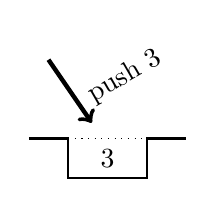
\begin{tikzpicture}
\phantom{\draw (0,1.4) -- (0,0);}
\draw[ultra thick,->] (0.25,1) -- (0.8,0.2) node [above right,rotate=30] {push 3};
\draw[thick] (0,0) -- (0.5,0) -- (0.5,-.5) -- (1.5,-.5) -- (1.5,0) -- (2,0);
\draw[dotted] (0.5,0) -- (1.5,0);
\node at (1,-0.25) {$3$};
\end{tikzpicture}}
&
\imagetop{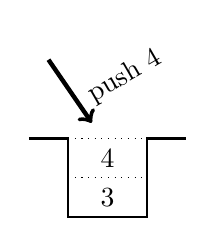
\begin{tikzpicture}
\phantom{\draw (0,1.4) -- (0,0);}
\draw[ultra thick,->] (0.25,1) -- (0.8,0.2) node [above right,rotate=30] {push 4};
\draw[thick] (0,0) -- (0.5,0) -- (0.5,-1) -- (1.5,-1) -- (1.5,0) -- (2,0);
\draw[dotted] (0.5,0) -- (1.5,0);
\draw[dotted] (0.5,-0.5) -- (1.5,-0.5);
\node at (1,-0.25) {$4$};
\node at (1,-0.75) {$3$};
\end{tikzpicture}}
&
\imagetop{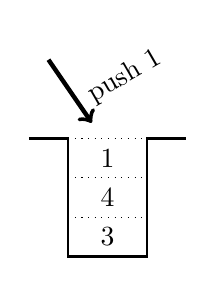
\begin{tikzpicture}
\phantom{\draw (0,1.4) -- (0,0);}
\draw[ultra thick,->] (0.25,1) -- (0.8,0.2) node [above right,rotate=30] {push 1};
\draw[thick] (0,0) -- (0.5,0) -- (0.5,-1.5) -- (1.5,-1.5) -- (1.5,0) -- (2,0);
\draw[dotted] (0.5,0) -- (1.5,0);
\draw[dotted] (0.5,-0.5) -- (1.5,-0.5);
\draw[dotted] (0.5,-1) -- (1.5,-1);
\node at (1,-0.25) {$1$};
\node at (1,-0.75) {$4$};
\node at (1,-1.25) {$3$};
\end{tikzpicture}}
&
\imagetop{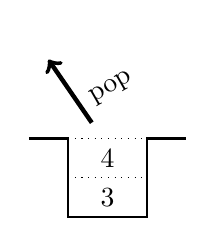
\begin{tikzpicture}
\phantom{\draw (0,1.4) -- (0,0);}
\draw[ultra thick,<-] (0.25,1) -- (0.8,0.2) node [above right,rotate=30] {pop};
\draw[thick] (0,0) -- (0.5,0) -- (0.5,-1) -- (1.5,-1) -- (1.5,0) -- (2,0);
\draw[dotted] (0.5,0) -- (1.5,0);
\draw[dotted] (0.5,-0.5) -- (1.5,-0.5);
\node at (1,-0.25) {$4$};
\node at (1,-0.75) {$3$};
\end{tikzpicture}}
\\
(empty) & top$=3$ & top$=4$ & top$=1$ & top$=4$
\end{tabular}}

\paragraph{使用上の注意}
通常は,配列や\texttt{vector}などが用いられる.
典型的な実装での計算コストは\texttt{push()},\texttt{pop()},\texttt{top()}とも定数時
間である.つまり,データがどれだけ増えても,各操作の計算時間は増えないと期待される.

なお,\texttt{pop()}が\texttt{top()}同様に値を返す実装もあるが,C++の
標準ライブラリで提供されているものはでは,両者が分離されていることに注意\footnote{こ
  れはexception safetyのためである.}.通常の使用状況では,先頭の要素を得つつスタックやキューからは取り除きたいので,両者の操作を
続けて行う.

また現在の要素数を調べる\texttt{size()}などのメンバ関数も提供されているので詳しくは文法書を参照のこと\footnote{ウェブにも資料がある\url{http://en.cppreference.com/w/cpp/container/stack}}.

\begin{cbox}[emph={stack,push,top,pop}]
#include <stack>
#include <iostream>
using namespace std;
int main() {
    stack<int> S; // intを格納するスタック
    S.push(3); // 先頭に追加
    S.push(4);
    S.push(1);
    while (! S.empty()) { // 要素がある間
	int n = S.top(); // 先頭をコピーして
	S.pop(); // 先頭要素を廃棄
	cout << n << endl; // 1, 4, 3  の順に表示される
    }
}  
\end{cbox}

Pythonでは\texttt{append, pop}をそれぞれ\texttt{push, pop}として用いる
ことにする.
\begin{pybox}[emph={append,pop}]
stack = []
stack.append(3)
stack.append(4)
stack.append(1)
while len(stack) > 0:
    n = stack.pop()
    print(n)
\end{pybox}

\begin{psbox}{Reverse Polish Notation}{AOJ}
「逆ポーランド記法」で与えられる文法を読んで、値を計算する
  
\aojid{ALDS1_3_A}
\end{psbox}

ヒント: 問題分末尾にある「解説」も参照.
\pcaojbook[p.82]に詳しい解説が掲載されている.

\begin{cbox}[emph={string,stack,top,push}]
#include <string>
#include <stack>
#include <iostream>
using namespace std;
int main() {
  string word;
  stack<int> S;
  while (cin >> word) { // 入力がある限り読み込む
    if (word == "+") {
      // 数を2つpopして、和をpushする
    }
    else if (word == "-") {
      // 数を2つpopして、差をpushする
    }
    else if (word == "*") {
      // 数を2つpopして、積をpushする
    }
    else {
      // wordを数値にしてpushする
    }
  }
  // Sの先頭要素を表示する。
}
\end{cbox}

このプログラムは入力が続くかぎり読み込む。キーボードから入力の終わりを
与えるには ``\textasciicircum{}D'' (Ctrlキーを押しながら ``d''を押す)を用いる。

数をあらわす文字列を整数\texttt{n}に変換するには、
C++11の場合は \texttt{int n=stoi(word)}を、
そうでない場合は \texttt{<cstdlib>} をincludeして、\texttt{int n=atoi(word.c\_str())}などとする。(AOJのC++11はまだ\texttt{stoi}をサポートしていないので\texttt{atoi}を用いる)

\begin{pbox}{Largest Rectangle in a Histogram}{Ulm Local 2003}
  ヒストグラム中に含まれる最大の長方形の面積を求めよ.(long long注意)

\url{http://poj.org/problem?id=2559}
\end{pbox}

スタックをうまく活用すると,ヒストグラムの本数に比例する手間で求められ
る.

参考: \url{http://algorithms.blog55.fc2.com/blog-entry-132.html}

\subsection{キュー}\label{section:queue}
\paragraph{概要} キュー(\eindex{queue},\pccbook[p.~32])は,
データの格納(\texttt{push()})と取り出し(\texttt{pop()})ができるデータ構造である.
現在先頭にあるデータは,\tindex{front}\texttt{()}で参照する.

\centerline{\begin{tabular}{c@{\hspace{2em}}c@{\hspace{2em}}c@{\hspace{2em}}c@{\hspace{2em}}c}
\imagetop{\begin{tikzpicture}
\phantom{\draw (0,1.0) -- (0,0);}
\draw[thick] (0,0) -- (2,0);
\end{tikzpicture}}
&
\imagetop{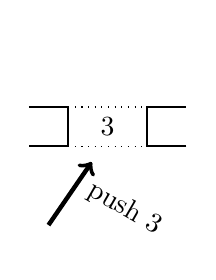
\begin{tikzpicture}
\phantom{\draw (0,1.0) -- (0,0);}
\draw[ultra thick,->] (0.25,-1.5) -- (0.8,-0.7) node [below right,rotate=-30] {push 3};
\draw[thick] (0,0) -- (0.5,0) -- (0.5,-.5) -- (0,-.5);
\draw[thick] (2,-.5) -- (1.5,-.5) -- (1.5,0) -- (2,0);
\draw[dotted] (0.5,0) -- (1.5,0);
\draw[dotted] (0.5,-0.5) -- (1.5,-0.5);
\node at (1,-0.25) {$3$};
\end{tikzpicture}}
&
\imagetop{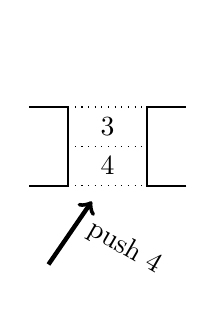
\begin{tikzpicture}
\phantom{\draw (0,1.0) -- (0,0);}
\draw[ultra thick,->] (0.25,-2) -- (0.8,-1.2) node [below right,rotate=-30] {push 4};
\draw[thick] (0,0) -- (0.5,0) -- (0.5,-1) -- (0,-1);
\draw[thick] (2,-1) -- (1.5,-1) -- (1.5,0) -- (2,0);
\draw[dotted] (0.5,0) -- (1.5,0);
\draw[dotted] (0.5,-0.5) -- (1.5,-0.5);
\draw[dotted] (0.5,-1) -- (1.5,-1);
\node at (1,-0.25) {$3$};
\node at (1,-0.75) {$4$};
\end{tikzpicture}}
&
\imagetop{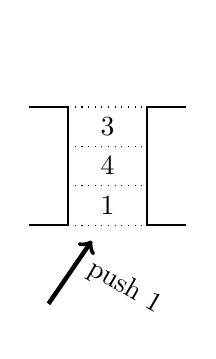
\begin{tikzpicture}
\phantom{\draw (0,1.0) -- (0,0);}
\draw[ultra thick,->] (0.25,-2.5) -- (0.8,-1.7) node [below right,rotate=-30] {push 1};
\draw[thick] (0,0) -- (0.5,0) -- (0.5,-1.5) -- (0,-1.5);
\draw[thick] (2,-1.5) -- (1.5,-1.5) -- (1.5,0) -- (2,0);
\draw[dotted] (0.5,0) -- (1.5,0);
\draw[dotted] (0.5,-0.5) -- (1.5,-0.5);
\draw[dotted] (0.5,-1) -- (1.5,-1);
\draw[dotted] (0.5,-1.5) -- (1.5,-1.5);
\node at (1,-0.25) {$3$};
\node at (1,-0.75) {$4$};
\node at (1,-1.25) {$1$};
\end{tikzpicture}}
&
\imagetop{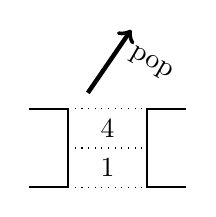
\begin{tikzpicture}
\phantom{\draw (0,1.0) -- (0,0);}
\draw[ultra thick,->] (0.75,0.2) -- (1.3,1) node [below right,rotate=-30] {pop};
\draw[thick] (0,0) -- (0.5,0) -- (0.5,-1) -- (0,-1);
\draw[thick] (2,-1) -- (1.5,-1) -- (1.5,0) -- (2,0);
\draw[dotted] (0.5,0) -- (1.5,0);
\draw[dotted] (0.5,-0.5) -- (1.5,-0.5);
\draw[dotted] (0.5,-1) -- (1.5,-1);
\node at (1,-0.25) {$4$};
\node at (1,-0.75) {$1$};
\end{tikzpicture}}
\\
(empty) & front$=3$ & front$=3$ & front$=3$ & front$=4$
\end{tabular}}

\paragraph{使用上の注意}
実装には,配列や\tindex{deque}が用いられる.
計算コストは\texttt{push()},\texttt{pop()},\texttt{front()}とも定数時
間である.つまり,データがどれだけ増えても,各操作の計算時間は増えないと期待される.
(データ全体を移動させると$O(N)$かかってしまうので,実際にはheadとtailのような現在使用中の区間をあらわす添字またはポインタのみを操作する).

C++では,queueというテンプレートクラスが用意されている.入れた(pushし
た)データを,front()及びpop()の操作により取り出す.\footnote{\url{http://en.cppreference.com/w/cpp/container/queue}}
\begin{cbox}[emph={queue,push,front,pop}]
#include <queue>
#include <iostream>
using namespace std;
int main() {
    queue<int> Q; // intを格納するキュー
    Q.push(3); // 末尾に追加
    Q.push(4);
    Q.push(1);
    while (! Q.empty()) { // 要素がある間
	int n = Q.front(); // 先頭をコピーして
	Q.pop(); // 先頭要素を廃棄
	cout << n << endl; // 3, 4, 1  の順に表示される
    }
}
\end{cbox}

Pythonのqueueの表現としては,この資料では\texttt{collections.deque}の\texttt{append, popleft}を用いることにする.\footnote{https://docs.python.jp/3/library/collections.html\#deque-objects}
\begin{pybox}[emph={append,popleft}]
import collections
q = collections.deque()
q.append(3)
q.append(4)
q.append(1)
while len(q) > 0:
    n = q.popleft() # 先頭から取り出す
    print(n)
\end{pybox}


\begin{psbox}{Round-Robin Scheduling}{AOJ}
複数の計算を少しづつ処理する様子をシミュレーションしてみよう。

\aojid{ALDS1_3_B}
\end{psbox}

ヒント: 問題分末尾にある「解説」も参照.\pcaojbook[p.82]に詳しい解説が掲載されている.

\begin{pbox}{Areas on the Cross-Section Diagram}{AOJ}
与えられた地形に雨が降った際に,できる水たまりの面積を出力する.

\aojid{ALDS1_3_D}
\end{pbox}

ヒント: 水面が形成されるとしたら,同じ高さの下りと上りの最近ペアである.
文字列を左から順に見て,
\begin{itemize}
\item \textcolor{white}{下りであれば位置をスタックに入れる}
\item \textcolor{white}{上りであれば,スタックの先頭要素である下りと対応させ,スタックから取り除く}
\end{itemize}
とすることで,同じ高さの下りと上りのペアをつくることが出来る.あとは,隠れてしまう水面を取り除くと良い.一例は,開始位置と面積を\texttt{pair<int,int>}で表現して\texttt{stack}で管理すること.

\begin{pbox}{Subsequence}{Southeastern Europe 2006}
配列Aの連続する部分列について,その和がS以上となるものので最小の長さを
求めよ.

\url{http://poj.org/problem?id=3061}
\end{pbox}

サンプルの解説: (10,7)の部分が合計$17 \ge 15$を満たし要素数2で最小.
(3,4,5)の部分が$12 \ge 11$を満たし要素数3で最小.

ヒント: 全ての区間を調べると$O(N^2)$かかるが,次のように合計が$S$に近い区間のみを調べると$O(N)$で処理することが出来る.配列の先頭要素から順に見て,キュー内部の要素の合計がS未満なら\texttt{push}して要素を増やし,S以上なら\texttt{pop}して減らす.キュー内部の要素の合計は,それを表す変数を設け,\texttt{push}や\texttt{pop}のタイミングで管理する.

いわゆるしゃくとり法. たぶん,cinだと遅いので,scanfを使う.

\begin{center}
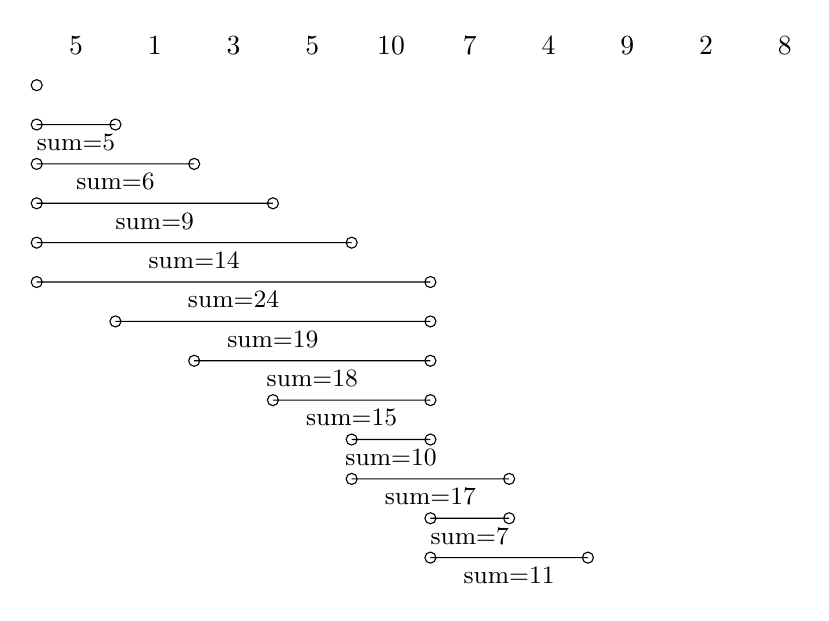
\begin{tikzpicture}
  \node at (0,0) {5};
  \node at (1,0) {1};
  \node at (2,0) {3};
  \node at (3,0) {5};
  \node at (4,0) {10};
  \node at (5,0) {7};
  \node at (6,0) {4};
  \node at (7,0) {9};
  \node at (8,0) {2};
  \node at (9,0) {8};

\draw (-0.5,-0.5) circle [radius=2pt,fill=black];
\draw (-0.5,-1.0) circle [radius=2pt,fill=black] -- node[below]
      {\small sum=5} (0.5,-1.0) circle [radius=2pt,fill=black];
\draw (-0.5,-1.5) circle [radius=2pt,fill=black] -- node[below] {\small sum=6} (1.5,-1.5) circle [radius=2pt,fill=black];
\draw (-0.5,-2) circle [radius=2pt,fill=black] -- node[below] {\small sum=9} (2.5,-2) circle [radius=2pt,fill=black];
\draw (-0.5,-2.5) circle [radius=2pt,fill=black] -- node[below] {\small sum=14} (3.5,-2.5) circle [radius=2pt,fill=black];
\draw (-0.5,-3) circle [radius=2pt,fill=black] -- node[below] {\small sum=24} (4.5,-3) circle [radius=2pt,fill=black];
\draw (0.5,-3.5) circle [radius=2pt,fill=black] -- node[below] {\small sum=19} (4.5,-3.5) circle [radius=2pt,fill=black];
\draw (1.5,-4) circle [radius=2pt,fill=black] -- node[below] {\small sum=18} (4.5,-4) circle [radius=2pt,fill=black];
\draw (2.5,-4.5) circle [radius=2pt,fill=black] -- node[below] {\small sum=15} (4.5,-4.5) circle [radius=2pt,fill=black];
\draw (3.5,-5) circle [radius=2pt,fill=black] -- node[below] {\small sum=10} (4.5,-5) circle [radius=2pt,fill=black];
\draw (3.5,-5.5) circle [radius=2pt,fill=black] -- node[below] {\small sum=17} (5.5,-5.5) circle [radius=2pt,fill=black];
\draw (4.5,-6) circle [radius=2pt,fill=black] -- node[below] {\small sum=7} (5.5,-6) circle [radius=2pt,fill=black];
\draw (4.5,-6.5) circle [radius=2pt,fill=black] -- node[below] {\small sum=11} (6.5,-6.5) circle [radius=2pt,fill=black];
\end{tikzpicture}
\end{center}

\begin{pbox}{Sum of Consecutive Prime Numbers}{アジア地区予選2005}
与えられた整数を,連続する素数の和として表せる種類を求めよ.

\aojid{1257}
\end{pbox}

初めにエラトステネスの篩(\pccbook{} 112ページ)などの手法で,$10\,000$までの素数を求めておく.
あとは
``Subsequence''と同じ.

\subsection{優先度付きキュー}\label{section:priority-queue}
優先度付きキュー(\eindex{priority queue}, \pccbook[p.~32])は,
データの格納と取り出しができるデータ構造で,
まだ取り出されていない中で大きな順に取り出されるものである.

\begin{psbox}{Priority Queue}{AOJ}
整数を入力として受け入れ、大きい順に取り出すことができる、優先度付き
キュー(priority queue)を作成せよ。

\aojid{ALDS1_9_C}
\end{psbox}

まずは,標準ライブラリ\texttt{priority\_queue}\footnote{\url{http://en.cppreference.com/w/cpp/container/priority_queue}}を用いて,acceptedを得られることを確認
すると良い.
自分で優先度つきキューを実装する場合は,配列または\texttt{vector}上に
二分ヒープ(binary heap)を作成することが簡便.詳しくは\pcaojbook[10章,pp.~232--]を参照.

\begin{cbox}[emph={queue,priority_queue,push,top,pop}]
#include <queue>
#include <iostream>
using namespace std;
int main() {
    priority_queue<int> Q; // intを格納する優先度つきキュー
    Q.push(3); // 追加
    Q.push(4);
    Q.push(1);
    while (! Q.empty()) { // 要素がある間
	int n = Q.top(); // 先頭をコピーして
	Q.pop(); // 先頭要素を廃棄
	cout << n << endl; // 4, 3, 1  の順に表示される
    }
}
\end{cbox}

Pythonには\texttt{heapq}パッケージがあるので,それを使うことにする.
\begin{pybox}
import heapq

Q = []
heapq.heappush(Q, 3)
heapq.heappush(Q, 4)
heapq.heappush(Q, 1)
while len(Q) > 0:
    n = heapq.heappop(Q)
    print(n)                    # 1,3,4の順に表示される
\end{pybox}



\section{文字列と分割・連結・反転}
C++では\texttt{string}\footnote{\url{http://en.cppreference.com/w/cpp/string/basic_string}}データの部分文字列を\texttt{substr}メソッド\footnote{\url{http://en.cppreference.com/w/cpp/string/basic_string/substr}}で得ることができる.
\begin{cbox}
  string word = "hello";
  for (size_t i=0; i<=word.size(); ++i) { // size() は文字列の長さ
    string l = word.substr(0,i);// i 文字目より左の文字列
    string r = word.substr(i); // i 文字目以降の文字列
    cout << l << ' ' << r << endl;
  }
\end{cbox}

実行例:\\
\begin{alltt}
 hello
h ello
he llo
hel lo
hell o
hello 
\end{alltt}

練習: \texttt{string word = "hello";}のhelloを別の単語にして動かしてみよう.

\begin{pybox}
word = "hello";
for i in range(len(word)+1):
    l = word[0:i]
    r = word[i:]
    print(l+' '+r)  
\end{pybox}

連結には,\texttt{+}オペレータを用いる.C++もrubyも同じ.

\begin{cbox}
    string a = "AAA";
    string b = "BBB";
    string c = a+b; // 連結
    cout << c << endl; // AAABBB
\end{cbox}

 反転には,
\texttt{reverse}という関数を用いる.範囲は\texttt{word.begin()}と\texttt{word.end()}で指定する.配列の場合と近い記法で,\texttt{reverse(\&word[0], \&word[0]+word.size());}と書くこともできる.
 
\begin{cbox}
#include <algorithm>
    string word = "hello";
    reverse(word.begin(), word.end());
    cout << word << endl;  
\end{cbox}

\section{集合 (set)}

C++で集合を表現するために標準ライブラリに\eindex{set}\footnote{\url{http://en.cppreference.com/w/cpp/container/set}}及び
\eindex{unordered\_set}\footnote{\url{http://en.cppreference.com/w/cpp/container/unordered_set}}(C++11以降)というデータ構造が標準が用意されている.
まずは整数の集合の例を紹介
する.
どちらもほぼ同じ操作を提供するが,ここでは挿入(\texttt{insert}),全体
の要素数(\texttt{size}),指定した要素の有無の検索(\texttt{count})を使用す
る.

実装において\texttt{set}は前者がデータに順序をつけて,
\texttt{unordered\_set}
は順序を無視して管理する.前者は通常二分探索木で実装され,挿入や検索に$O(\log N)$の時間が必要である.すなわち,データ数$N$とともに一回の操作は遅くなることに注意.後者は通常ハッシュ表を使って実装され,各操作は平均的には定数時間でおさまると期待される.


\begin{cbox}[emph={set}]
#include <set>
    typedef set<int> set_t;
    set_t A;
    cout << A.size() << endl; // 初めは空なので0
    cout << A.count(3) << endl; // 3は含まれていないので0
    A.insert(1);
    A.insert(3);
    A.insert(5);
    A.insert(3);
    cout << A.size() << endl; // 1,3,5の3つ
    cout << A.count(3) << endl; // 1個 (setの場合は最大1個)
    cout << A.count(4) << endl; // 0個
\end{cbox}

文字列の集合も同様に使うことができる.

\begin{cbox}[emph={set,string}]
#include <set>
#include <string>
    typedef set<string> set_t;
    set_t A;
    cout << A.size() << endl; // 初めは空なので0
    cout << A.count("hello") << endl; // "hello"は含まれていないので0
    A.insert("hello");
    A.insert("world");
    A.insert("good morning");
    A.insert("world");
    cout << A.size() << endl; // "hello", "good morning", "world"
    cout << A.count("world") << endl; // 1個 setの場合は最大1
    cout << A.count("hello!!!") << endl; // 0個
\end{cbox}

pythonの場合は\texttt{set}が用意されている.\footnote{\url{https://docs.python.jp/3/library/stdtypes.html\#set}}
\begin{pybox}
s = set()
print('a' in s)                 # False
s.add('a')
print('a' in s)                 # True
s.discard('a')
print('a' in s)                 # False
\end{pybox}


\begin{psbox}{Search - Dictionary}{AOJ}
単語が辞書にある単語かどうかを判定せよ

\aojid{ALDS1_4_C}
\end{psbox}

\begin{tipsbox}{Time Limit Exceeded?}
Time Limit Exceeded (TLE)という判定でACを得られなかった場合,それは実行時間が許容範囲を越えたことを意味する.
C++で\texttt{set}を使っている場合は,\texttt{unordered\_set}を使ってみよう.その場合,提出ウィンドウで言語をC++ではなくC++11を選択する.
\end{tipsbox}

\subsection{bitset}
集合の特殊な場合として,0からNまでの整数の集合を扱う場合は,ビット表現を用いると効率が良い.C++では標準で\tindex{bitset}型が用意されている.

\begin{cbox}
#include <bitset>
#include <assert>
betset<128> a, b, c;
a[3] = 1; // 指定したbitをonに
b[5] = 1;
c = a | b; // 集合の和
\end{cbox}

\section{連想配列 (map)}

個人番号に対する名前を管理する場合には,配列を用いることが一般的である.

\begin{cbox}
string name[30];
name[0] = "kaneko";
name[1] = "fukuda";
\end{cbox}

では,名前に対する個人番号を管理するにはどうすれば良いか.

\begin{cbox}
number["kaneko"] = 0; // こんなふうに書きたい
\end{cbox}

連想配列とは,\texttt{key}に対する\texttt{value}を管理する抽象データ型
で,上記のような機能を提供する.C++では\eindex{map}\footnote{\url{http://en.cppreference.com/w/cpp/container/map}}と\eindex{unordered\_map}\footnote{\url{http://en.cppreference.com/w/cpp/container/unordered_map}}, Pythonでは\texttt{dict}\footnote{\url{https://docs.python.jp/3/library/stdtypes.html\#dict}}が標準で用意されている.

\subsection{文字列に対応する数字}

\begin{cbox}[emph={map}]
#include <iostream>
#include <string>
#include <map>
using namespace std;
int main() {
  map<string,int> table; // 文字列を数値に対応させるmap
  table["taro"] = 180;
  table["hanako"] = 160;
  cout << table["taro"] << endl; // 180
  cout << table["ichirou"] << endl; // 0
}  
\end{cbox}

このような例では,\texttt{key}が文字列,\texttt{value}が整数である.

\begin{pybox}
all = {}
print(len(all))                 # 0
all["hello"] = 1
all["world"] = 100
all["good morning"] = 20
print(len(all))                 # 3
for k,v in sorted(all.items()):
    print("
# good morning 20
# hello 1
# world 100
\end{pybox}

\begin{psbox}{English Sentence}{PC甲子園2004}
与えられた文字列について,出現頻度が最も高い単語と,最も文字数が多い単語を出力する

\aojid{0029}
\end{psbox}


\texttt{string}型の文字列\texttt{s} の長さは \texttt{s.size()} で入手することができる.

\subsection{文字列の出現回数}

\texttt{key}が存在しない場合の振る舞いは,処理系と設定に依存するが,上
記の例では0になるように用いている.
これにより出現回数の計測を簡単に行うことができる.

\begin{cbox}
  table["ichirou"]+=1;
  cout << table["ichirou"] << endl; // 1
  table["ichirou"]+=1;
  cout << table["ichirou"] << endl; // 2
\end{cbox}

\begin{pybox}
# 普通のhashの利用
table = {}  
# table["ichirou"] += 1 ... ng!
table["ichirou"] = table.get("ichirou", 0) + 1
if not "world" in table:
   table["world"] = 1
# Counterの利用
import collections
c = collections.Counter()
c["ichirou"] += 1 # ok
\end{pybox}

\subsection{連想配列の要素の一覧}

\begin{c11box}[emph={map,iterator,begin,end,first,second}]
  map<string,int> phone;
  phone["taro"] = 123;
  phone["jiro"] = 456;
  phone["saburo"] = 789;

  for (auto p=phone.begin(); // i=0に相当
       p!=phone.end(); // i$<$Nに相当
       ++p) {
      cout << p->first << " " << p->second << endl;
  }
// 出力順は
// jiro 456
// saburo 789
// taro 123
\end{c11box}

赤字で書いた部分が定型句であるが,初見では把握が難しいため,そのまま用いてほ
しい.配列の場合は添字として整数\texttt{i}を用いるが,連想配列の場合は
複雑な処理があるため,整数の代わりにイテレータと呼ばれる抽象インターフェースを用いる.\footnote{ここではC++11の機能を利用して,\texttt{auto}と書いた.実際の方は\texttt{map<string,int>::iterator}であるる.}また初期値と終了値も,$0$や$N$の代わりに\texttt{begin()}と\texttt{end()}
を用いる.ループの中で,各要素の\texttt{key}は\texttt{p->first}, \texttt{value}は\texttt{p->second}で参照する.


\section{練習問題}
\begin{pbox}{Organize Your Train part II}{国内予選2006}
貨物列車の並べ替え.何通りの可能性があるか?

\aojid{1142}
\end{pbox}

\begin{cbox}
int M;
string S;
int main() {
    cin >> M;
    for (int i=0; i<M; ++i) {
        cin >> S;
        ... all; // 文字列の集合
        ... // allにSを挿入
        for (size_t i=1; i<S.size(); ++i) {
            string L;
            ... // LをSの[0,i)文字に設定
            string R;
            ... // RをSの[i,S.length())文字に設定
            string L2, R2;
            ... // L2をLの逆順に設定
            ... // R2をRの逆順に設定
            ... // allにR+L, R2+L, L+R2..色々挿入
        }
        ... // allの要素数(all.size())を出力
    }
}  
\end{cbox}

\begin{pbox}{Era Name}{模擬地区予選2010}
(架空の)西暦と(架空の)元号の対応が与えられるので,整理して記憶する.
続いて,西暦が質問として与えられるので,元号がわかっていれば元号を,そ
うでなければ ``Unknown'' と答える.

\aojid{2242}
\end{pbox}

問題補足: 入力例の"showa 62 1987"は,
\begin{itemize}
\setlength{\itemsep}{0pt}
\item 昭和元年(1年)の西暦は,1926年である
\item 昭和は,(少なくとも)1987年まで続いた
\end{itemize}
という二つの情報をあらわす.
他に情報がなければ,1988年が昭和であるかは分からない(昭和と平成の間に別の元号が使われているかもしれない)ので,
 ``Unknown'' と答える.

回答例: 各情報を,西暦とその年が1年である元号の対応表と,元号が最大何年まで続いたかの二つに分けて記録する.
前者には\texttt{map<int,string>}を,後者には\texttt{map<string,int>}を用いる.




\subsection{区間の管理}

\begin{pbox}{Restrictive Filesystem$\star$}{模擬国内予選2009}

単純な管理を行うファイルシステムでの,読み書きと消去を実装し,各時点で読まれるデータを答えよ.

\aojid{2152}
\end{pbox}

回答例: \textcolor{white}{ディスクの状態を,区間\texttt{pair<int,int>}とファイルのIDを対応させる連想配列
\texttt{map<pair<int,int>, int>}で表現して,読み書きと消去をシミュレートする.}

\subsection{集合の応用}

\begin{pbox}{Twenty Questions$\star$}{アジア地区予選2009}
それぞれのobjectを区別するのに,最善の質問の仕方を考える.答え次第で次の質問を変えて良い.

\aojid{1302}
\end{pbox}

\begin{pbox}{Sweets$\star$}{Algorithmic Engagements 2010}
正の数が$n\le24$個ある.兄弟$A,D,B$でそれらを分ける.$A\ge D\ge B$を満たす分け方の中で,$A-B$が最小の分け方を探す.

\url{https://szkopul.edu.pl/problemset/problem/cEMM4bdcKN06uikzs9BRSqkz/site/}
\end{pbox}

解説されている解法を担当者が実装したつもりのものでもtleなので(最大ケース5秒くら
い), ``Useful Resources''からデータをダウンロードして正しければ時間は気にしないことが良さそう.

\begin{pbox}{Building Blocks$\star$}{15th Polish Olympiad in Informatics}
$N$本の棒グラフがある.どこか連続する$K(\le N)$本を選んで,同じ高さに揃えたい.
高さを1増やすのも減らすのも同じコストがかかる.コストの総和の最小とその時の各棒グラフの高さを出力せよ.

\url{https://szkopul.edu.pl/problemset/problem/KC7c6nYfAXCbCGszqhIeOGxP/site/}
\end{pbox}

入出力はscanfでなくcinを用いても問題ない.STLのデータ構造の組み合わせで解くことができる.

\chapter{グラフ(1) 全域木}

\begin{itembox}[l]{概要}
本日から複数回,グラフの話題を扱う.グラフは,様々な状況や問題をモデル化するための,基礎となる概念である.
今週は,最小重み全域木を求めてみよう.またそのための道具として,
グループを管理する Disjoint Set (Union-Find Tree) というデータ構造を紹介する.
\end{itembox}

\section{グラフと木}

接続関係に焦点をあてて世の中をモデル化する際に,グラフがしばしば用いら
れる.
路線図,物流,血縁関係,などなど.
(\pccbook[2-5節, p.~87] あれもこれも実は``グラフ'')

\begin{center}
      \begin{tikzpicture}[node distance=15mm]
        \node[city] (A)              {$a$};
        \node[city] (B) [below of=A] {$b$};
        \node[city] (C) [below of=B] {$c$};
        \node[city] (D) [right of=B] {$d$};
        \path[thick] (A) edge (B);
        \path[thick] (B) edge (C);
        \path[thick] (C) edge (D);
        \path[thick] (D) edge (B);
      \end{tikzpicture}
\end{center}


\subsection{グラフに関する用語}

\jindex{グラフ}{ぐらふ}は,\jindex{頂点}{ちょうてん} (点,\jindex{節点}{せってん},\eindex{vertex}; 複数形は vertices)と\jindex{辺}{へん}
(枝,線,\eindex{edge}, \eindex{arc})からなる.
頂点集合 $V$ と辺集合$E$でグラフ$G=(V,E)$を表す.

例: 3つの頂点$V=\{1,2,3\}$の辺を全て結んだグラフ(=三角形)は,
$E=\{\{1,2\},\{2,3\}, \{3,1\}\}$

頂点$v$と辺$e$に対して$v\in e$となる時,$v$は$e$に\textbf{接続}する.
頂点$v$に対して,$v$の接続辺の個数$|E(v)|$を\jindex{次数}{じすう}(\eindex{degree}) という.
二つの頂点が共通の接続辺を持つ場合にその頂点は\textbf{隣接}するという.
隣接する頂点をリストにして並べたものを\jindex{パス}{ぱす} (\eindex{path}, trail, walk
で細かくは異なる意味を持たせるので,詳しく学ぶ際には注意)と呼ぶことにする.

例: 三角形の各頂点の次数は2


\subsection{木}

特殊な(連結で閉路がない)グラフを\textbf{木}という.木は,一般のグラフより扱いや
すい.
木で表せるものには,式(3 + (5 - 2)),階層ファイルシステム(リンクなどを除く),自分の祖先を表す家系図(いとこなど血縁間の結婚がない場合),インターネットのドメイン名などがある.

\begin{center}
  \begin{tabular}{c@{\hspace{3em}}cc}
\imagetop{\begin{forest}
  ctree [ a ]
    \end{forest}}
&
\imagetop{\begin{forest}
  ctree [ a [ b ] [ c ] [ d ] ]
    \end{forest}}
&
\imagetop{\begin{forest}
  ctree [ a [b] [ c [ d] [e]]]
    \end{forest}}
\\
木1 & 木2 & 木3
  \end{tabular}
\end{center}

\paragraph{定義}

無向グラフ$G$に対して,全ての2頂点$v,w$に対して$v-w$パスが存在する時に$G$を\textbf{連結}と呼ぶ.
閉路を含まないグラフを\jindex{森}{もり} (\eindex{forest})または\textbf{林}と呼ぶ.
連結な森を\jindex{木}{き}(\eindex{tree})という. 

グラフ$T$の頂点数が$n$として,$T$が木であることと以下は同値である:
\begin{itemize}
\item $T$は$n-1$個の辺からなり,閉路を持たない
\item $T$は$n-1$個の辺からなり,連結である
\item $T$の任意の2頂点に対して,2頂点を結ぶパスが一つのみ存在する
\item $T$は連結で,$T$のどの辺についても,それを$T$から取りのぞいたグラフは非連結
\item $T$は閉路を含まず,$T$の隣接しない2頂点を$xy$をどのように選んでも,$xy$をつなぐ辺を$T$に加えたグラフは閉路を含む
\end{itemize}

木の頂点の特別な一つを\jindex{根}{ね} (\eindex{root})と呼ぶ.
グラフを図示する際には,根を一番上または下に配置することが多い.次数1
の点を\jindex{葉}{は} (\eindex{leaf})と呼ぶ.
木の辺で結ばれた2頂点について,根に近い方の頂点(あるいは根)を
\jindex{親}{おや} (parent)と呼び,遠い方を\jindex{子}{こ} (child)と呼ぶ.

\subsection{「親」に注目した,木の表現}

$N$個の節点を持つ「木」を計算機上で表す方法の一つに,各節点に$1$から
$N$までの数字の番号をふり,各節点の親を一次元配列(以下,parent の頭文字
を用いてP[]と表記する)で管理する方法がある.木には,たかだか1つの親を持つという性
質がある.そこで,節点$i$に対応する$P[i]$の数値に,節点$i$が親を持つ場
合にはには親の番号,親を持たない場合(すなわち\textbf{根}(root))には$-1$または自分自身などの特殊な番号を割り当てる.

なお,木ではない一般のグラフでは,各節点で子を複数持ちうるので,子を管理する場合は一次元配列より複雑な表現(隣接リスト,隣接行列など\ref{section:adjacency-matrix})が必要となる.

\begin{center}
  \begin{tabular}{lc@{\hspace{3em}}cc}
木&
\imagetop{\begin{forest}
  ctree [ 1 ]
    \end{forest}}
&
\imagetop{\begin{forest}
  ctree [ 1 [2][3][4] ]
    \end{forest}}
&   
\imagetop{\begin{forest}
  ctree [ 5 [2][3[4][1]] ]
    \end{forest}}
\\
配列表現&
\begin{tabular}{c|c}
i & 1 \\
P[i] & 1
\end{tabular}
&
\begin{tabular}{c|cccc}
i & 1 & 2 & 3 & 4\\
P[i] & 1 & 1 & 1 & 1
\end{tabular}
&
\begin{tabular}{c|ccccc}
i & 1 & 2 & 3 & 4 & 5\\
P[i] & 3 & 5 & 5 & 3 & 5
\end{tabular}
  \end{tabular}
\end{center}


\section{Disjoint Set (Union-Find Tree)}
二つの要素が同一グループに属するかどうかを効率的に判定する手法の一つが、
\eindex{Union Find}木 (\pcaojbook[pp.~318--], \pccbook[pp.~81--])である。\eindex{Disjoint-set}とも呼ばれる。
グループ同士を併合する操作ができるが,分離はできない(c.f. link-cut tree).

\begin{center}
  \begin{forest}
    [,rootempty [1] [2] [3 [4]] [5 [6] [7 [8 [9]]]]]
  \end{forest}
\\
\begin{tabular}{c|ccccccccc}
   i & 1 & 2 & 3 & 4 & 5 & 6 & 7 & 8 & 9\\
P[i] & 1 & 2 & 3 & 3 & 5 & 5 & 5 & 7 & 8
\end{tabular}\\
$\{1\}, \{2\}, \{3,4\}, \{5,6,7,8,9\}$の4つのグループ
\end{center}

\paragraph{判定}
同じ木に属するなら同じグループで,そうでなければ異なるグループである.
それを,根(root)を調べることで行う.
例:
\begin{itemize}
\setlength{\itemsep}{0pt}
\item \textbf{Q1. 6と8は同じグループに属するか?}\\
6の属する木の根(root)は5で,同様に8の根は5 \dingright{} 同じグループ.
\item \textbf{Q2. 2と4は同じグループに属するか?}\\
2の属する木の根は2で,4の根は3 \dingright{} 異なるグループ.
\end{itemize}
 
\paragraph{併合}

併合は,二つの節点を同一グループにまとめる操作で,一方の節点の属する木
の根をもう一方の節点の属する木の根につなげることで実現する.
どちらをどちらにつなげても,意味は変わらない.(小さな(低い)木を大きな(高い)木の下につける方が効率が良い,が,この資料では割愛する)

\begin{center}
  \begin{tabular}{c@{\hspace{2em}}c}\hline
\imagetop{\begin{forest}
     [,rootempty [1] [2]]
  \end{forest}}
&
\imagetop{\begin{forest}
ctree [1 [2]]
  \end{forest}}
\\
\begin{tabular}{c|cc}
   i & 1 & 2\\
P[i] & 1 & 2
\end{tabular}
&
\begin{tabular}{c|cc}
   i & 1 & 2\\
P[i] & 1 & \cemph{1}\end{tabular}
\\
元のグラフ & 1と2を併合したグラフ\\\hline

\\
\imagetop{\begin{forest}
    [,rootempty,for tree={s sep=10mm} [3 [4,rtree]] [5 [6] [7 [8,rtree [9,ctree]]]]]
  \end{forest}}
&
\imagetop{\begin{forest}
ctree [5,for tree={s sep=10mm}, [3 [4]] [6] [7 [8 [9]]]]
  \end{forest}}
\\
\begin{tabular}{c|ccccccc}
   i & 3 & 4 & 5 & 6 & 7 & 8 & 9\\
P[i] & 3 & 3 & 5 & 5 & 5 & 7 & 8
\end{tabular}
&
\begin{tabular}{c|ccccccc}
   i & 3 & 4 & 5 & 6 & 7 & 8 & 9\\
P[i] & \cemph{5} & 3 & 5 & 5 & 5 & 7 & 8
\end{tabular}
\\
元のグラフ & 4と8を併合したグラフ\\
&(グループ全体を併合するためには根同士を接続)\\\hline
  \end{tabular}
\end{center}


\paragraph{効率化: パス圧縮}

節点の根を求める操作は,根からの距離が遠いほど時間がかかる.
そこで,一度根を調べたら,関係する接点をなるべく根に直接つなげるようにつなぎ替えると効率の改善に有効である.

\begin{tabular}{c@{\hspace{5em}}c}
\imagetop{\begin{forest}
ctree [5 [3 [4]] [6] [7 [8[9,rtree]]]]
  \end{forest}}
&
\imagetop{\begin{forest}
ctree [5 [3 [4]] [6] [7,rtree] [8,rtree][9,rtree]]
  \end{forest}}
\\
\begin{tabular}{c|ccccccc}
   i & 3 & 4 & 5 & 6 & 7 & 8 & 9\\
P[i] & 5 & 3 & 5 & 5 & 5 & 7 & 8
\end{tabular}
&
\begin{tabular}{c|ccccccc}
   i & 3 & 4 & 5 & 6 & 7 & 8 & 9\\
P[i] & 5 & 3 & 5 & 5 & \cemph{5} & \cemph{5} & \cemph{5}
\end{tabular}
\\
元のグラフ & root(9) = 5を調べたついでに木を変形
\end{tabular}

\paragraph{コード例:}
以下に,初期化,判定,併合のコード例を示す.なお,初見でコードの理解が難しい場合は,
一度書き写して動作を試した後に再度理解を試みるのが良い.(\texttt{rank}の概念は無視している.)

\begin{cbox}[emph={root,is\_same\_set,unite}]
int P[10010]; // 0から10000までの頂点を取り扱い可能
void init(int N) { // 初期化 はじめは全ての頂点はバラバラ
    for (int i=0; i<N; ++i) P[i] = i;
}
int root(int a) { // aのroot(代表元)を求める
    if (P[a] == a) return a; // aはroot
    return (P[a] = root(P[a])); // aの親のrootを求め,aの親とする
}
bool is_same_set(int a, int b) { // aとbが同じグループに属するか?
    return root(a) == root(b);
}
void unite(int a, int b) { // aとbを同一グループにまとめる
    P[root(a)] = root(b);
}
\end{cbox}
関数\texttt{root}の最後で\texttt{P[a]}に代入している部分が,パス圧縮である.

\begin{pybox}[emph={root,is\_same\_set,unite}]
P = [i for i in range(N)]
def root(x):
    path_to_root = []
    while P[x] != x:
        path_to_root.append(x)
        x = P[x]
    for node in path_to_root:
        P[node] = x  # パス圧縮
    return x
def is_same_set(x,y):
    return root(x) == root(y)
def unite(x,y):
    P[root(x)] = root(y)
\end{pybox}
Pythonでは,再帰の深さの制限がC++よりきついので,関数\texttt{root}を再帰ではなく\texttt{while}で実装しておく.


実行例:

\begin{cbox}
int main() {
  init(100);
  cout << is_same_set(1, 3) << endl;
  unite(1,2);
  cout << is_same_set(1, 3) << endl;
  unite(2,3);
  cout << is_same_set(1, 3) << endl;
}\end{cbox}

\begin{psbox}{Disjoint Set: Union Find Tree}{AOJ}
Disjoint Setでグループを管理せよ

注意: $S_1,\ldots,S_k$の集合の添字は無視すること.とくに「$x$ を含む集合 $S_x $」の$S_x$と対応するわけではない.

\aojid{DSL_1_A}
\end{psbox}

\section{全域木}

連結なグラフ$G$の頂点全てと辺の全てまたは一部分を用いて構成される木を
\jindex{全域木}{ぜんいきぎ} (\eindex{spanning tree})または\textbf{全点木}と呼ぶ.
辺に重みがついている場合に,全域木に含まれる辺の重みの合計が最小であるような木を
\jindex{最小(重み)全域木}{さいしょうぜんいきぎ} (\eindex{minimum spanning tree})と呼ぶ.

メモ: グラフが連結なら全域木が存在する.全域木は一つとは限らない(完全グラフの場合は$n^{n-2}$個もある).最小全域木も一つとは限らない.最小全域木を求める問題は,最小全域木のうちの一つを求める問題を指すことが多い.


\begin{center}
  \begin{tabular}{c@{\hspace{2em}}c@{\hspace{2em}}c@{\hspace{2em}}c}
      \begin{tikzpicture}[node distance=15mm]
        \node[city] (A)              {$a$};
        \node[city] (D) [right of=A] {$d$};
        \node[city] (B) [below of=A] {$b$};
        \node[city] (C) [right of=B] {$c$};
        \path[thick] (A) edge (B);
        \path[thick] (B) edge (C);
        \path[thick] (C) edge (A);
        \path[thick] (C) edge (D);
        \path[thick] (D) edge (A);
      \end{tikzpicture}
&
      \begin{tikzpicture}[node distance=15mm]
        \node[city] (A)              {$a$};
        \node[city] (D) [right of=A] {$d$};
        \node[city] (B) [below of=A] {$b$};
        \node[city] (C) [right of=B] {$c$};
        \path[ultra thick, draw=ired] (A) edge (B);
        \path[thick] (B) edge (C);
        \path[thick] (C) edge (A);
        \path[ultra thick, draw=ired] (C) edge (D);
        \path[ultra thick, draw=ired] (D) edge (A);
      \end{tikzpicture}
&
      \begin{tikzpicture}[node distance=15mm]
        \node[city] (A)              {$a$};
        \node[city] (D) [right of=A] {$d$};
        \node[city] (B) [below of=A] {$b$};
        \node[city] (C) [right of=B] {$c$};
        \path[thick] (A) edge (B);
        \path[ultra thick, draw=ired] (B) edge (C);
        \path[thick] (C) edge (A);
        \path[thick] (C) edge (D);
        \path[ultra thick, draw=ired] (D) edge (A);
      \end{tikzpicture}
&
      \begin{tikzpicture}[node distance=15mm]
        \node[city] (A)              {$a$};
        \node[city] (D) [right of=A] {$d$};
        \node[city] (B) [below of=A] {$b$};
        \node[city] (C) [right of=B] {$c$};
        \path[thick] (A) edge (B);
        \path[ultra thick, draw=ired] (B) edge (C);
        \path[ultra thick, draw=ired] (C) edge (A);
        \path[ultra thick, draw=ired] (C) edge (D);
        \path[ultra thick, draw=ired] (D) edge (A);
      \end{tikzpicture}
\\
元のグラフ &
赤い部分グラフは全域木 & 全域木でない(非連結) & 全域木でない(閉路)
  \end{tabular}
\end{center}

\subsection{クラスカル法}

最小重み全域木を求める方法として,有名な方法にプリム法(Prim)と\jindex{クラスカル法}{くらすかるほう} (\eindex{Kruskal})があるが,ここでは後者を紹介する.

クラスカル法は以下のように動作する (\pccbook[pp.~101--]):
\begin{itemize}
\setlength{\itemsep}{0pt}
\item 辺を重みの小さい順にソートする (数字の組をソートする方法は\ref{section:sort-pairs}章を参照)
          \begin{itemize}
          \item 方法1: $\langle$ 重み, 始点, 終点$\rangle$をソート
          \item 方法2: $\langle$ 重み, 辺ID$\rangle$をソートし,IDと始点や終点を対応させる配列を別に管理
          \end{itemize}
\item $T$を作りかけの森 (最初は空,閉路を含まないグラフ,連結とは限らない)とする
\item 重みの小さい順に,各辺$e$に対して以下の操作を行う\\
 $T+e$ (グラフ$T$に辺$e$を加えたグラフ)が閉路を含まなければ$T$に$e$を加える
\end{itemize}

\begin{center}
  \begin{tabular}{c@{\hspace{2em}}c@{\hspace{2em}}c@{\hspace{2em}}c}
      \begin{tikzpicture}[node distance=15mm]
        \node[city] (A)              {$a$};
        \node[city] (D) [right of=A] {$d$};
        \node[city] (B) [below of=A] {$b$};
        \node[city] (C) [right of=B] {$c$};
        \path[thick] (A) edge node [left] {4} (B);
        \path[thick] (B) edge node [below] {5} (C);
        \path[thick] (C) edge node [above] {3} (A);
        \path[thick] (C) edge node [right] {2} (D);
        \path[thick] (D) edge node [above] {1} (A);
      \end{tikzpicture}
&
      \begin{tikzpicture}[node distance=15mm]
        \node[city] (A)              {$a$};
        \node[city] (D) [right of=A] {$d$};
        \node[city] (B) [below of=A] {$b$};
        \node[city] (C) [right of=B] {$c$};
        \path[thick] (A) edge node [left] {4} (B);
        \path[thick] (B) edge node [below] {5} (C);
        \path[thick] (C) edge node [above] {3} (A);
        \path[thick] (C) edge node [right] {2} (D);
        \path[ultra thick, draw=ired] (D) edge node [above] {1} (A);
      \end{tikzpicture}
&
      \begin{tikzpicture}[node distance=15mm]
        \node[city] (A)              {$a$};
        \node[city] (D) [right of=A] {$d$};
        \node[city] (B) [below of=A] {$b$};
        \node[city] (C) [right of=B] {$c$};
        \path[thick] (A) edge node [left] {4} (B);
        \path[thick] (B) edge node [below] {5} (C);
        \path[thick] (C) edge node [above] {3} (A);
        \path[ultra thick, draw=ired] (C) edge node [right] {2} (D);
        \path[ultra thick, draw=ired] (D) edge node [above] {1} (A);
      \end{tikzpicture}
&
      \begin{tikzpicture}[node distance=15mm]
        \node[city] (A)              {$a$};
        \node[city] (D) [right of=A] {$d$};
        \node[city] (B) [below of=A] {$b$};
        \node[city] (C) [right of=B] {$c$};
        \path[ultra thick, draw=ired] (A) edge node [left] {4} (B);
        \path[thick] (B) edge node [below] {5} (C);
        \path[thick] (C) edge node [above] {3} (A);
        \path[ultra thick, draw=ired] (C) edge node [right] {2} (D);
        \path[ultra thick, draw=ired] (D) edge node [above] {1} (A);
      \end{tikzpicture}
\\
元のグラフ &
辺ad (重み1)を採用 & 辺cd (重み2)を採用 & 辺ab (重み4)を採用
  \end{tabular}
\end{center}

$T+e$が閉路を含むかどうかを効率的に判定する手法の一つが,union-find treeである.
上記のクラスカル法内で,辺$e$を加える度に\texttt{unite}で辺の両端の頂点を同一グループに組み込む.
辺$e$の両端を$a,b$として,\texttt{is\_same\_set(a,b)}が真であれば辺$e$を加えると閉路ができる($e$と別に$a,b$パスがあるので).

\begin{psbox}{Graph II - Minimum Spanning Tree}{AOJ}
与えられたグラフの最小全域木の重みの総和を求めよ.

\aojid{ALDS1_12_A}
\end{psbox}

\begin{pbox}{Stellar Performance of the Debunkey Family}{PC甲子園2008}
問題: 街を連結に保ったまま,橋の維持費用を最小化したい.

\aojid{0180}  
\end{pbox}

\paragraph{入出力例}
入力を読み込んで,維持コストの少ない辺の順番に出力するコードは,たとえば以下のように作ることができる.今日の主眼は,クラスカル法の実習にあるので,これをそのままコピーしても問題ない.

\begin{cbox}
#include <algorithm>
int N, M, A[10010], B[10010], COST[10010];
pair<int,int> bridge[10010]; // コストと橋番号のペア
int main() {
    while // (N と M を読み込み,Nが0より大きければ処理する) {
        for (int i=0; i<M; ++i) {
            // A[i] と B[i] と COST[i] を読み込む;
            bridge[i].first = COST[i];
            bridge[i].second = i;
        }
        sort(bridge, bridge+M); // コストの小さい順に整列
        for (int i=0; i<M; ++i) {
            int cost = bridge[i].first;
            int a = A[bridge[i].second];
            int b = B[bridge[i].second];
            // 「aからbにcostの橋がかかっている」と表示
        }
    }
}
\end{cbox}

コード中の\texttt{pair<int,int>}とは\texttt{struct pair \{ int first, second; \};}に相当.

\paragraph{回答例:} 上記の準備ができているとして,回答の骨子は以下のようになる.

\begin{cbox}
        int 合計 = 0;
        for (int i=0; i<M; ++i) { //安い橋から順に
            if // (端の両端の節点が既に連結だったら)
                continue;
            // 橋の両端の節点を同一グループに併合する;
            // 合計に,橋のコストを加える;
        }
        // 合計を出力;
\end{cbox}

\section{練習問題}

\begin{pbox}{Marked Ancestor}{夏合宿2009}
マークされている最も近い祖先を求める.初めは根だけがマークされている.

注意: 合計はintを越えるので,long longを用いる.

  \aojid{2170}
\end{pbox}

補足: 下記の図で,初めに「猫」の ``nearest marked ancestor''は「動物」,もし「哺乳類」がマークされた後なら,「猫」の ``nearest marked ancestor''は「哺乳類」.

\begin{center}
\begin{forest}
ctree [動物 [両生類 [蛙]] [爬虫類] [哺乳類 [猫][犬]]]
\end{forest}
\end{center}

\begin{tipsbox}{ヒント}
まず,MarkやQueryなどの命令列を全て読み込み,\textcolor{white}{後ろからマークを
外してゆくように処理してゆくとすると...?}
\end{tipsbox}

\subsection{Disjoint Sects}
\begin{pbox}{Fibonacci Sets}{会津大学プログラミングコンテスト2003}
i番目のFibonacci数をf[i]と表記する.
あるi, j ($1\le i,j \le V$)について,f[i]\%1001とf[j]\%1001の差の絶対値がd未満だったら,ノードiとjは同じグループに属するとする.Vとdが与えられた時に,グループの数を数えよ.

\aojid{1016}
\end{pbox}

回答例:
\begin{cbox}
int F[1001];
int main() {
    F[0] = 1, F[1] = 2;
    // ... F[i]に i番目の Fibonacci数\%1001 をあらかじめ計算,代入しておく
    while (cin >> V >> D) {
        // 木を初期化
        for (int i=1; i<=V; ++i)
            for (int j=i+1; j<=V; ++j)
                if // (F[j] と F[i]の差の絶対値が D未満だったら)
                    // グループiとグループjを同一化;
        // i\(\in\)[1,V]に関してroot(i) == iであるような数を数えて出力
    }
}  
\end{cbox}

細かく作ってテストする:
\begin{itemize}
\setlength{\itemsep}{0pt}
\item Fibonacci数の計算: F[2]..F[1000]までを for 文で代入する(\ref{section:fibonacci}の方針3で\texttt{a[2]}の代わりに\texttt{F}を用いることと,1001の剰余を取りながら行う点が差).
つまり,iを小さい方から大きくしてゆけば,定義通りに\texttt{F[i] = F[i-2]+F[i-1];} と計
算できる.オーバーフローしないように計算途中でも1001の剰余を取る.
(表示して確認する)
\item Union-find木を作る: 基本的には資料通り\\
(初期化して,木を表示して確認する.いくつか併合しては木を表示して確認する.)
\item Fibonacci数での動作作成: 小さなV(たとえば10)と適当なDを与えて,
  木を表示し,手計算と一致するかどうかをテストする.
\item グループの数を数える: root(i) == i である個数ををテストする.
\end{itemize}


\begin{pbox}{True Liars}{アジア地区予選2002}
真実のみいう人(=正直者)と嘘だけ言う人住む島があって,それぞれの合計人数はわかっ
ている.
「人xが人yを正直者である/ない」と言ったという情報を総合して,割り当てが一意に定まるならばそれを求めよ.

\aojid{1238}
\end{pbox}

\begin{tipsbox}{ヒント}
正直者かどうかが直接的には分からなくても,\textcolor{white}{正直者か嘘つきかどちらかに共通に属する複数の人物の情報が分かる場合がある.そのような人を集めてグループ化する.各グループについて正直者かそうでないかを割り当ててみる.}
\end{tipsbox}

\begin{pbox}{Never Wait for Weights$\star$}{アジア地区予選2012}
(意訳)要素が属するグループだけでなく,要素間の距離を管理せよ.

\aojid{1330}
\end{pbox}

回答方針: 根との距離をデータに加えたUnion-find木を作れば良い.

\begin{pbox}{Everlasting --One--$\star$}{アジア地区予選2013}
転職できる仕事をグループにして,行き来できないグループがどれだけあるかを知りたい.

\aojid{2568}
\end{pbox}



\subsection{色々な全域木}

\begin{pbox}{Slim Span$\star$}{アジア大会2007}
  最小の辺の重みと最大の辺の重みの差が最小の全域木を求めよ.

  \aojid{1280}
\end{pbox}
\begin{tipsbox}{ヒント}
  全域木の最大の辺の重みについて考える.クラスカル法は,\textcolor{white}{
    最大の辺の重みが最小である木を出力する.そこで,最小の重みを
    $a$を全通り試しながら,重み$a$未満の辺を無視したクラスカル法の出力
    を吟味すれば良い.なお元のグラフが連結でない場合は,全域木を作れない可能性もある.クラスカル法が停止した時点で,
    disjoint setの代表元が全ての頂点で同一であることを確認すると良い.}
\end{tipsbox}

\begin{pbox}{Sinking islands$\star$}{模擬国内予選2013}

沈みゆく島にどのように(問題文参照)橋をかけるかを求める.
  
  \aojid{2511}
\end{pbox}


\begin{pbox}{Byteland$\star$}{1st Junior Polish Olympiad in Informatics}
同じ重みの辺が存在する場合は,最小重み全域木は複数通り存在しうる.
各辺毎にminimum spanning treeに含まれうるかを調べる

\url{https://szkopul.edu.pl/problemset/problem/JXaPu39wQfiZaqlM51zlchez/site/}
\end{pbox}

時間制限は最大15秒確保されれているようだが,1.5秒くらいで解ける.
クラスカル法が正しい解を与える証明と関連.

\begin{pbox}{There is No Alternative$\star$}{アジア地区予選2014}
どのような最小重み全域木を作っても必ず使う辺を求める.

  \url{http://judge.u-aizu.ac.jp/onlinejudge/cdescription.jsp?cid=ICPCOOC2014&pid=F}

c.f. 類題 \url{http://codeforces.com/problemset/problem/160/D}
\end{pbox}

\section{補足: 木に関連する他の話題}
\subsection{最小共通祖先}

\begin{center}
  \begin{forest}
sn edges [動物,s sep=15mm [両生類 [蛙]] [爬虫類] [哺乳類 [猫] [犬]]]
  \end{forest}
\end{center}

ある木について,木の二つの節点に共通する祖先でもっとも近い節点を
最小共通祖先 (lowest common ancestor) と呼んで LCA と略す.
図の例で,犬と猫のLCAは哺乳類.蛙と犬のLCAは動物.

\begin{psbox}{Nearest Common Ancestors}{Taejon 2002}
一つの木と,その木の節点が二つ与えられる.二つの節点に共通するもっとも
近い祖先を求めよ.
  
\url{http://poj.org/problem?id=1330}
\end{psbox}

いくつかのステップに分割して解いてみよう:
\begin{enumerate}
\item 入力を目で理解する. 一行目に数字Tがあり,「木の情報とLCAを求める節点
  二つ」がTセット続いている.Sample Inputの木を紙に書いてみる.
\item 木の入力を読み込む
各P[]を表示して確認せよ.
各節点の親は,紙に描いた木と一致するか?
\item LCAを求める準備として,ある節点xから根までの節点を全て求めること
  を考える.
考え方としては,xの親はP[x]で求められるから,親の親,親の親の親などとたどっていけばいずれは根に到達する.親をたどる際に節点を表示して,確認してみよう.
\item 節点AとBのそれぞれについて,根までのパス(頂点番
  号列)の共通要素を求める.一番根から遠いものが求める答え.
\end{enumerate}


なお,発展的な話題になるが,一つの木について何度もLCAを求める場合には,事前に準備をしておくと一回あたり$O(\log{}N)$と効率的に求められる(\ref{section:RMQ}章や\pccbook[p.~274]を参照).
\begin{pbox}{Apple Tree$\star$}{POJ Monthly--2007.08.05}

りんごの数を数える

\url{http://poj.org/problem?id=3321}
\end{pbox}



\subsection{親への移動}

\begin{pbox}{Marbles on a tree}{Waterloo local 2004.06.12}

N個の節点を持つ木が与えられる.
木の各節点には,果物がない場合と,一つあるいは複数の果物がある場合があ
る.果物の合計はN個である.
各節点が一つづつ果物を持つようにするためには,最低何回の移動が必要か.
一つの果物を一つの辺にそって移動すると1回と数える.
  
\url{http://poj.org/problem?id=1909}
\end{pbox}


入力のサンプルコードを示す:
\begin{cbox}
#include <cstdio>
using namespace std;
int N, P[10010], M[10010], V[10010];
int main() {
    while (~scanf("
        fill(P, P+N, -1);
        int /*葉の数*/L=0, id, c;
        for (int i=0; i<N; ++i) {
            scanf("
            scanf("
            for (int j=0; j<V[id]; ++j) {
                scanf("
                P[c] = id;
            }
            if (V[id] == 0) ++L; // Vが0ならidは葉
        }
        for (int i=0; i<N; ++i) {
            // 親を出力してみる
            printf("
        }
    }
}
\end{cbox}
(pojはcinを使うと時間制限になる問題があるため,scanfを勧める)

\paragraph{方針:} 各節点について親から/へ移動する果物を考える.たとえ
ば親から3つもらって5つ返すのは無駄で,それなら差し引き2つ送るだけで良
い.つまり,各節点について,まずは子供の間で不足と余剰の調整を行ない,
残った分を親に調整を依頼すると良い.

\begin{cbox}
  // 節点が調整済みかを表す配列を用意する.初めに葉を調整済みとしておく.
  // 各節点での過不足を表す配列を用意する.初期値は,果物の配置数-1
  while // 根が調整済みでない {
    for // 全ての節点iについて {
      if // iが調整済みでない かつ iの子供が全て調整済みなら {
        // iでの過不足を親に押し付ける
        // iを調整済みと記録
      }
    }
  }
  // 各節点での過不足の合計が答え
\end{cbox}

\begin{figure}
\centering
\begin{forest}
  ctree [ 1(2) [2(1)] [3(0) [5(3)][6(0)]] [4(1) [7(0)][8(2)][9(0)]] ]
  \end{forest}
  \caption{Sample 1}
  \label{figure:samlpe1}
\end{figure}

\begin{figure}
\centering
\begin{forest}
  ctree [ 1(1) [2(0)] [3(-1) [5(2)][6(-1)]] [4(0) [7(-1)][8(1)][9(-1)]] ]
  \end{forest}
  \caption{Sample 1(過不足)}
  \label{figure:samlpe1-adjust}
\end{figure}

\begin{figure}
\centering
\begin{forest}
  ctree [ 1(1) [3(0)] [4(-1)] ]
  \end{forest}
  \caption{葉を調整(2=0, 5=2, 6=-1, 7=-1, 8=1, 9=-1を消去)}
  \label{figure:samlpe1p}
\end{figure}


\subsection{木と動的計画法}
この節以降は\ref{section:graphsearch}章のグラフの探索に馴染んでから取り組むことが適切.

\begin{pbox}{TELE$\star$}{Croatia OI 2002 Final Exam - Second Day}
(意訳) 放送局が番組を配信する計画を立てる.受信できた場合に視聴者が払う
額はあらかじめ与えられる.配信路は木構造になっている.木の節点は,根が放送
局自身,葉が視聴者.他が中継装置である.赤字にならずに配信できる人数は何人か?

(筆者注) 各コストCの制約がないが,正で5000以下の模様.

\url{http://poj.org/problem?id=1155}
\end{pbox}

ヒント: 節点\texttt{i}から\texttt{j}人に配信するコスト\texttt{T[i][j]}のようなものを管理しながら根から深さ優先探索を行う.各節点で,たとえば二つの子を持つ内部節点で3人に配信する場合の収益は、
(0,3), (1,2),... (3,0)のようなすべての割り当ての中から最大を選ぶ必要があ
る.

\begin{pbox}{Heap$\star\star$}{POJ Monthly--2007.04.01}
ノードに整数が書かれた二分木がある.整数を書き換えて,どのノードに対
しても,(左の子孫たち) $<$ (右の子孫たち) $\le$
(自分自身) を満たすようにしたい.最小何か所書き換えればよいか?

木は完全二分木とは限らず,後ろのほうが詰まっていない場合がある.

\url{http://poj.org/problem?id=3214}
\end{pbox}
入力形式注意

\subsection{木の直径}

\begin{pbox}{Fuel$\star$}{Algorithmic Engagements 2011}
木と,歩いて良い辺の数が与えられるので,訪れる頂点の数を最大化した観光
ツアーを設計せよ (walk; 同じ辺を複数回通って良い,始点と終点は別で良い)

\url{https://szkopul.edu.pl/problemset/problem/5g0vDW-MvMGHfWQqh56jQKx1/site/}
\end{pbox}

\begin{pbox}{Bridge Removal$\star$}{国内予選2014}
群島の橋を渡りながら全ての橋を撤去しながら職人の,最短時間を求める.

\aojid{1196}
\end{pbox}

\subsection{木の正規化}

\begin{pbox}{部陪博士,{\scriptsize あるいは,われわれはいかにして左右非対称になっ
    たか}$\star\star$}{国内予選 2007}
式を表す二分木を与えられた規則で正規化せよ

\aojid{1152} 
\end{pbox}

(面倒なので経験者向け.なお,ICPCではなるべく端末専有時間を短く解くことが求められる)


\subsection{木の中心}

\begin{pbox}{Cave$\star\star$}{11th Polish Olympiad in Informatics}
木の節点のどこかに宝が隠されている。質問に対する答えを元にその宝を見つける.
質問回数を最小にするような質問戦略で必要になる、最大の質問回数を求めよ.

質問は,節点を一つ選んで,そこに宝があるかを聞く.
宝がある場合はそこでゲームが終了し,そうでない場合は,どちら方向に宝が
あるかが隣接する節点により示される.

\url{https://szkopul.edu.pl/problemset/problem/5Z9PRRPP-R90WhmbSY_qHd-1/site/}
\end{pbox}


\begin{versionalpha}
\section{グラフのその他の概念}
グラフの辺をちょうど一回づつ通
る閉路/パスを
\eindex{Euler circuit}/trail (\jindex{オイラー閉路}{おいらーへいろ}/路)}という. 

判定法: 連結であること,全ての頂点の次数が偶数であること/パスの始点と終点を除いて偶数であること.

\begin{center}
  \begin{tabular}{c@{\hspace{3em}}cc}
      \begin{tikzpicture}[node distance=15mm]
        \node[city] (A)              {$a$};
        \node[city] (B) [below of=A] {$b$};
        \node[city] (C) [right of=B] {$c$};
        \path[thick] (A) edge (B);
        \path[thick] (B) edge (C);
        \path[thick] (C) edge (A);
      \end{tikzpicture}
&
      \begin{tikzpicture}[node distance=15mm]
        \node[city] (A)              {$a$};
        \node[city] (D) [right of=A] {$d$};
        \node[city] (B) [below of=A] {$b$};
        \node[city] (C) [right of=B] {$c$};
        \path[thick] (A) edge (B);
        \path[thick] (B) edge (C);
        \path[thick] (C) edge (A);
        \path[thick] (C) edge (D);
        \path[thick] (D) edge (A);
      \end{tikzpicture}
&
      \begin{tikzpicture}[node distance=15mm]
        \node[city] (A)              {$a$};
        \node[city] (D) [right of=A] {$d$};
        \node[city] (B) [below of=A] {$b$};
        \node[city] (C) [right of=B] {$c$};
        \path[thick] (A) edge (B);
        \path[thick] (B) edge (C);
        \path[thick] (C) edge (A);
        \path[thick] (C) edge (D);
        \path[thick] (D) edge (A);
        \path[thick] (B) edge (D);
      \end{tikzpicture}
\\
Euler閉路あり(e.g., abca) & 閉路はないが全ての辺を辿れる (adcabc) & 全ての辺をたどれない
  \end{tabular}
\end{center}

\begin{psbox}{Patrol}{PC甲子園2005}
問題: パトロールする街路を一筆書きで辿れるかを判定せよ.始点と終点は指定されている.連結であることは保証されている.

\aojid{0086}
\end{psbox}

\textbf{回答例}

\begin{cbox}
int main() {
    while (cin >> a >> b) { // 辺 a,b を読み込む
        ... // 頂点aの次数を増やす
        ... // 頂点bの次数を増やす
        if (a == 0) {
           ... // 始点から終点に一筆書き出来るか(*)を判定して出力
                // (*) 頂点番号1と2の字数が奇数,かつ,
                // 頂点番号3以上の頂点の次数が全て偶数
           // 次のテストケースのために,全ての頂点の次数を0に戻す
        }
    }
}
\end{cbox}

\begin{pbox}{Play on Words}{Central Europe 1999}
単語が与えられるので,全ての単語を「しりとり」で繋げられるかを判定せよ.
初めと終わりの単語は自由に選んで良い.
(連結であることは保証されていない)

筆者注: 時間制限が厳しいので入力にはscanfを使うと良い

\url{http://poj.org/problem?id=1386}  
\end{pbox}

\paragraph{回答例}
アルファベットを頂点としたグラフを考える.
たとえば\texttt{news}という単語を,頂点\texttt{n}から\texttt{s}への辺
と考える.ここで反対向きには使えないことから,(先ほどと異なり)辺に向き
がある(有向グラフという).

有向グラフの次数は,辺の向きに対応して,\textbf{入次数} (in-degree)と\textbf{出次数}(out-degree)を区別して扱う.

有向グラフがオイラー閉路を持つ必要十分条件は,
連結であることと,全ての頂点の入次数と出次数が等しいことである.
閉路でない場合は,パスの始点/終点で入次数が出次数より一つ多い/少ない.

問題Aと異なり,連結性が保証されないので,自分で判定する.(\ref{section:graphsearch}章参照)
\end{versionalpha}
 \chapter{グラフ(2) グラフ上の探索}\label{section:graphsearch}

\begin{itembox}[l]{概要}
連結なグラフの辺を全てたどる方法として,幅優先探索 (BFS)と深さ優先探索(DFS)を紹介する.
全部の辺をたどることから,グラフの\cemph{連結性}を判定したり,二部グラフかどうかを判定することが出来る.幅優先探索はさらに,根から各節点への距離を求めたり,木の直径を求めることができる.深さ優先探索は,トポロジカルソート,橋や間接点を求める,強連結成分分解などの応用がある.
\end{itembox}


\section{グラフの表現: 隣接リストと隣接行列}\label{section:adjacency-matrix}

各節点の親を覚えておくと木構造で親をたどることができたが,一般のグラフの節点を訪問するためには,より便利なデータが必要となる.

\paragraph{隣接行列}
初めに,グラフを\jindex{隣接行列}{りんせつぎょうれつ}(adjacency matrix)で表現する方法を紹介する.
節点$i$から$j$への辺が存在する時,行列の$i$行目$j$列目の値を$1$に,そうでないときに$0$とする.
辺に向きのない,無向グラフを扱う場合には行列は対称になる.

\begin{center}
\begin{tabular}{cc}
  \begin{minipage}{.2\linewidth}
\begin{tikzpicture}[node distance=15mm]
        \node[city] (A)              {$a$};
        \node[city] (B) [below of=A] {$b$};
        \node[city] (C) [below of=B] {$c$};
        \node[city] (D) [right of=B] {$d$};
        \path[thick] (A) edge (B);
        \path[thick] (B) edge (C);
        \path[thick] (C) edge (D);
        \path[thick] (D) edge (B);
      \end{tikzpicture}
  \end{minipage}
&
  \begin{minipage}{.4\linewidth}
\begin{tikzpicture}[>=latex]
\matrix (A) [matrix of math nodes,
             left delimiter  = (,
             right delimiter = )] at (0,0)
{
        0 & \node[circle](ab){1}; & 0 & 0\\
        \node[circle](ba){1}; & 0 & \node[circle](bc){1}; & \node(bd){1};\\
        0 & 1 & 0 & 1\\
        0 & 1 & 1 & 0\\
};

\matrix (R) [row sep=0.1mm] at (4.5,0)
{
        \node(abex){$a \to b$};\\
        \node {$\cdots$};\\
        & \node(baex){$b \to a$};\\
        & \node(bcex){$b \to c$};\\
        & \node {$\cdots$};\\
};
\draw[ired,->] (ab) to[in=160,out=20]  (abex);
\draw[ired,->] (ba) to[in=160,out=20]  (baex);
\draw[ired,->] (bc) to[in=160,out=20]  (bcex);
\end{tikzpicture}
  \end{minipage}
\end{tabular}
\end{center}

左のグラフの$a,b,c,d$をそれぞれ$0,1,2,3$の数値に対応させると,隣接行列は右のようになる.
すなわち$0,1,2,3$\textcolor{red}{行}目が$a,b,c,d$\cemph{から}出る辺を表し,
$0,1,2,3$\cemph{列}目が$a,b,c,d$\cemph{に}入る辺を表す.

なお,辺のコストや経路の数などを表すために,行列の要素に$1$以外の値を今後使うこともある.

グラフの表現の中で,隣接行列は比較的「贅沢な」グラフの表現方法である.都市
の数を$N$とすると,常に$N^2$に比例するメモリを使用する.

\paragraph{隣接リスト}

\jindex{隣接リスト}{りんせつりすと}は,接続先の頂点リストを図のような
リストで表す.実際には,頂点名$a$,$b$,$c$,$d$は頂点番号$0$,$1$,$2$,$3$
を用いると管理が容易である.C++の場合は頂点数を$N$として
\texttt{vector<int> edges[N];}として,\texttt{edges[i]}が$i$番目の頂点の接続先を表すようにする.先の章で辺のコストを管理する場合は,行き先とコストをペアにして,\texttt{vector<pair<int,int>> edges[N];}などとする.

\begin{center}
\begin{tikzpicture}[>=latex]
\matrix (A) [matrix of math nodes] at (0,0)
{
  a & \to & b \\
  b & \to & a & c & d \\
  c & \to & b & d \\
  d & \to & b & c \\
};
\end{tikzpicture}
\end{center}

隣接リストは,辺の数に比例したメモリを使用する.
グラフが疎な場合,すなわち辺の数が$N^2$よりもかなり少ない場合は,
隣接行列で値が$0$である要素が多くなり無駄が多い.
たとえば「木」の場合は,辺の
数は$N-1$しかない.
また,現実のグラフも電車の路線図のように,頂点に比べて辺が疎であることが多い.
隣接リストは,そのようなグラフに適する.
(参考: \pcaojbook[pp.~264--(12章)], \pccbook[pp.~90,~91])

\begin{psbox}{Graph}{AOJ}
有向グラフの隣接リストが与えられるので,隣接行列に変換する.

初めにグラフの節点の数$N$が与えられ,それに続いて$N$行が与えられる.各行は一つの節点に対応し,その節点から出ている辺を表す.初めの数$u$が節点の番号,続く数$k$が辺の数,その後に続く$k$個の数が各辺の行き先に対応している.(各行に含まれる数字の個数は,行毎に異なりうる)

  \aojid{ALDS1_11_A}
\end{psbox}

この問題のように多くのケースでは,頂点番号を$1,\ldots,N$でつけている.
一方,C++などでは配列の添字は0から始まるので,この資料では頂点番号から1を引いて,$0,\ldots,N-1$と内部では扱い,入出力の際に$\pm 1$して対応する.
Pythonによる回答例を示す.この資料では,問題文中に出てくる変数を(あとで値を変更する必要がない場合は)大文字で表記し定数として扱う.
\begin{pybox}
N = int(input())
G = [[0 for _ in range(N)] for _ in range(N)] # NxNの2次元配列
for _ in range(N):
    u,k,*varray = map(int,input().split()) # u,kは数, varrayは配列
    for v in varray:
        # Gにおいてu-1とv-1をつなげる
for row in G:
    print(' '.join(map(str,row))) # Gの各行を出力
\end{pybox}

\section{幅優先探索 (BFS)}\label{section:bfs}

\begin{pbox}{Breadth First Search}{AOJ}
節点1を始点に幅優先探索を行い,各節点の始点からの距離を表示せよ

(入力の形式は例題 ``Graph''と同じ)

\aojid{ALDS1_11_C}
\end{pbox}

幅優先探索(\pcaojbook[pp.~282--], \pccbook[p.~36])は,出発地に近い頂点から順に訪問する.

\begin{center}
\begin{tabular}{c@{\hspace{3em}}c}
      \begin{tikzpicture}[node distance=15mm,baseline=0cm]
        \node[city] (A)              {1};
        \node[city] (B) [below of=A] {2};
        \node[city] (C) [right of=A] {3};
        \node[city] (D) [right of=B] {4};
        \path[thick,->,out=-125,in=135] (A) edge (B);
        \path[thick,->] (A) edge (D);
        \path[thick,->,out=-35,in=-135] (B) edge (D);
        \path[thick,->,out=55,in=-45] (D) edge (C);
      \end{tikzpicture}
&
      \begin{tikzpicture}[node distance=15mm,baseline=0cm]
        \node[city,label=above right:{t=1}] (A) {1};
        \node[city,label=above right:{t=2}] (B) [below of=A] {2};
        \node[city,label=above right:{t=3}] (D) [right of=B] {4};
        \node[city,label=above right:{t=4}] (C) [below of=D] {3};
        \node (d2) [right of=C] {\colorbox{blue!10}{$d=2$}};
        \node (d1) [above of=d2] {\colorbox{blue!10}{$d=1$}};
        \node (d0) [above of=d1] {\colorbox{blue!10}{$d=0$}};
        \path[thick,->] (A) edge (B);
        \path[thick,->] (A) edge (D);
        \path[thick,->,dotted,gray] (B) edge (D);
        \path[thick,->] (D) edge (C);
        \draw[dotted] (-0.5,-.5) -- (4,-.5);
        \draw[dotted] (-0.5,-2) -- (4,-2);
      \end{tikzpicture}
      \\
      入力のグラフ(サンプル入力) & 幅優先探索の作る木
\end{tabular}
\end{center}

問題のサンプル入力である図の左に示したグラフが入力として与えられたとして,頂点$1$を始点に幅優先
探索を行った例を右に示す.右図の木の各節点の添字$t$は訪問時刻,実線は
幅優先探索中に使われた辺,点線は無視された辺を表す.$d$は始点からの距
離である.幅優先探索において,距離が等しい頂点の訪問順序は任意である.

このような探索を実現するために,
キューというデータ構造(\ref{section:queue}章参照)を用いる.キューに入れた(pushした)データは,
front()及びpop()の操作により早く入れた順に取り出される.
\begin{enumerate}
\item 始点から各頂点$n$への距離$d_{n}=\infty$と設定
\item キューに始点を入れる.(始点から)始点への距離を設定: $d_{\text{始点}}=0$
\item キューが空でない間,以下を繰り返す
  \begin{enumerate}
  \item キューの先頭の頂点$n$を取り出す
  \item $n$から移動可能な各頂点$n'$について,$d_{n'}=\infty$であれば(初めて見つけた頂点なので)以下を行う
    \begin{enumerate}
    \item $n'$をキューに入れる
    \item $n'$への距離を設定: $d_{n'}=d_n+1$
    \end{enumerate}
  \end{enumerate}
\end{enumerate}


この問題の入力の形式は例題 ``Graph''と同じで,サンプル入力も全く同じなので,
入力は作成済で,\texttt{G[s][t]==1}の時に(かつその時に限り),節点\texttt{s}から節点\texttt{t}に移動可能とする.

\begin{pybox}
import collections
D = [-1 for _ in range(N)]
D[0] = 0 # 始点への距離は0, 他の距離は-1
Q = collections.deque()
Q.append(0)                     # 始点
while len(Q) > 0:
    print("bfs", Q) # 各ステップでのQの動作を確認 (後で消すこと)
    cur = Q.popleft()
    for dst in range(N):
        if ...: # curからdstに移動可能かつ、dstが未訪問だったら \label{code:bfspy:visit}
            D[dst] = D[cur]+1
            Q.append(dst) # Qにdstを詰める
for v in range(N):
    print(v+1, D[v])        # [0,N-1]から[1,N]に変換
\end{pybox}

実行例は以下のようになる
\begin{alltt}
bfs deque([0])
bfs deque([1, 3])
bfs deque([3])
bfs deque([2])
1 0
2 1
3 2
4 1
\end{alltt}

BFSの過程で,キューには始点から辿れる節点が順に,各一度だけ,入れられる.
\ref{code:bfspy:visit}行目の条件で,dstが未訪問かどうかを判別しないと,合流やループがあるグラフで問題が生じる,
(たとえば1から2に辺があり,2から1にも辺がある場合に,1-2-1-2-1と移動し続け無限ループしてしまう).未訪問かどうかは,D[dst]を見ると判別できる.\textcolor{white}{この場合は,初期値-1が更新されているかどうか.}

\begin{cbox}[emph={queue,bfs,Q}]
#include <queue>
int D[...];
void bfs(int src) {
    cerr << "bfs root = " << src << endl;
    queue<int> Q; // 整数を管理するキューの定義
    Q.push(src);
    D[src] = 0; // 出発点
    while (! Q.empty()) {
        int cur = Q.front(); // 先頭要素を取り出す
        Q.pop();
        // 動作確認用表示
        cerr << "visiting " << cur << ' ' << D[cur] << endl;
        for (...) { // 各行き先 dst に対して
            if (..) { // curからdstに辺があり,dstが未訪問なら
                D[dst] = D[cur]+1; // 
                Q.push(dst); // dstを訪問先に加える
            } 
        }
    }
}  
\end{cbox}


\section{深さ優先探索 (DFS)}\label{section:dfs}

\begin{pbox}{Depth First Search}{AOJ}
番号の若い順に節点を深さ優先探索で訪問する時に,その訪問順序を表示せよ

「未発見の頂点が残っていれば、その中の1つを新たな始点として探索を
続けます。」ことに注意.

(入力の形式は例題 ``Graph''と同じ)

\aojid{ALDS1_11_B}
\end{pbox}

深さ優先探索(\pcaojbook[pp.~273--], \pccbook[p.~33])は,全ての節点を訪問する別の手法で,現在訪問中の頂点に近い頂点から順に訪問する.
まずは再帰的手続きを用いた実装を紹介する.

\begin{center}
  \begin{tabular}{c@{\hspace{2em}}c}
      \begin{tikzpicture}[node distance=15mm]
        \node[ccity](C1)               {$1$};
        \node[city] (C2) [right of=C1] {$2$};
        \node[city] (C3) [below of=C2] {$3$};
        \node[city] (C4) [right of=C2] {$4$};
        \node[city] (C5) [right of=C3] {$5$};
        \node[city] (C6) [right of=C5] {$6$};
        \path[thick,->] (C1) edge (C2);
        \path[thick,->] (C1) edge (C3);
        \path[thick,->] (C2) edge (C3);
        \path[thick,->] (C2) edge (C4);
        \path[thick,->] (C3) edge (C5);
        \path[thick,->] (C4) edge (C6);
        \path[thick,->] (C5) edge (C6);
      \end{tikzpicture}
&
      \begin{tikzpicture}[node distance=15mm]
        \node[vcity](C1)               {$1$};
        \node[ccity] (C2) [right of=C1] {$2$};
        \node[city] (C3) [below of=C2] {$3$};
        \node[city] (C4) [right of=C2] {$4$};
        \node[city] (C5) [right of=C3] {$5$};
        \node[city] (C6) [right of=C5] {$6$};
        \path[thick,->] (C1) edge (C2);
        \path[thick,->] (C1) edge (C3);
        \path[thick,->] (C2) edge (C3);
        \path[thick,->] (C2) edge (C4);
        \path[thick,->] (C3) edge (C5);
        \path[thick,->] (C4) edge (C6);
        \path[thick,->] (C5) edge (C6);
        \draw[thick,->,ired] (C1) to [out=45,in=135] (C2);
      \end{tikzpicture}\\
時刻1: 頂点1から開始 & 時刻2: 行き先候補2と3から2を選択\\
      \begin{tikzpicture}[node distance=15mm]
        \node[vcity](C1)               {$1$};
        \node[vcity](C2) [right of=C1] {$2$};
        \node[ccity](C3) [below of=C2] {$3$};
        \node[city] (C4) [right of=C2] {$4$};
        \node[city] (C5) [right of=C3] {$5$};
        \node[city] (C6) [right of=C5] {$6$};
        \path[thick,->] (C1) edge (C2);
        \path[thick,->] (C1) edge (C3);
        \path[thick,->] (C2) edge (C3);
        \path[thick,->] (C2) edge (C4);
        \path[thick,->] (C3) edge (C5);
        \path[thick,->] (C4) edge (C6);
        \path[thick,->] (C5) edge (C6);
        \draw[thick,->,ired] (C1) to [out=30,in=150] (C2);
        \draw[thick,->,ired] (C2) to [out=300,in=60] (C3);
      \end{tikzpicture}
&
      \begin{tikzpicture}[node distance=15mm]
        \node[vcity] (C1)               {$1$};
        \node[vcity] (C2) [right of=C1] {$2$};
        \node[vcity] (C3) [below of=C2] {$3$};
        \node[city]  (C4) [right of=C2] {$4$};
        \node[vcity] (C5) [right of=C3] {$5$};
        \node[ccity] (C6) [right of=C5] {$6$};
        \path[thick,->] (C1) edge (C2);
        \path[thick,->] (C1) edge (C3);
        \path[thick,->] (C2) edge (C3);
        \path[thick,->] (C2) edge (C4);
        \path[thick,->] (C3) edge (C5);
        \path[thick,->] (C4) edge (C6);
        \path[thick,->] (C5) edge (C6);
        \draw[thick,->,ired] (C1) to [out=30,in=150] (C2);
        \draw[thick,->,ired] (C2) to [out=300,in=60] (C3);
        \draw[thick,->,ired] (C3) to [out=30,in=150] (C5);
        \draw[thick,->,ired] (C5) to [out=30,in=150] (C6);
      \end{tikzpicture}
\\
時刻3: 同様に3を選択 & 時刻5: 同様に6まで進むと行き先がなく\\
      \begin{tikzpicture}[node distance=15mm]
        \node[vcity](C1)               {$1$};
        \node[vcity] (C2) [right of=C1] {$2$};
        \node[vcity] (C3) [below of=C2] {$3$};
        \node[city] (C4) [right of=C2] {$4$};
        \node[ccity] (C5) [right of=C3] {$5$};
        \node[vcity] (C6) [right of=C5] {$6$};
        \path[thick,->] (C1) edge (C2);
        \path[thick,->] (C1) edge (C3);
        \path[thick,->] (C2) edge (C3);
        \path[thick,->] (C2) edge (C4);
        \path[thick,->] (C3) edge (C5);
        \path[thick,->] (C4) edge (C6);
        \path[thick,->] (C5) edge (C6);
        \draw[thick,->,ired] (C1) to [out=30,in=150] (C2);
        \draw[thick,->,ired] (C2) to [out=300,in=60] (C3);
        \draw[thick,->,ired] (C3) to [out=30,in=150] (C5);
        \draw[thick,->,ired] (C5) to [out=30,in=150] (C6);
        \draw[thick,->,iblue] (C6) to [out=210,in=330] (C5);
      \end{tikzpicture}
&
      \begin{tikzpicture}[node distance=15mm]
        \node[vcity](C1)               {$1$};
        \node[vcity](C2) [right of=C1] {$2$};
        \node[vcity](C3) [below of=C2] {$3$};
        \node[ccity](C4) [right of=C2] {$4$};
        \node[vcity](C5) [right of=C3] {$5$};
        \node[vcity](C6) [right of=C5] {$6$};
        \path[thick,->] (C1) edge (C2);
        \path[thick,->] (C1) edge (C3);
        \path[thick,->] (C2) edge (C3);
        \path[thick,->] (C2) edge (C4);
        \path[thick,->] (C3) edge (C5);
        \path[thick,->] (C4) edge (C6);
        \path[thick,->] (C5) edge (C6);
        \draw[thick,->,ired] (C1) to [out=30,in=150] (C2);
        \draw[thick,->,ired] (C2) to [out=300,in=60] (C3);
        \draw[thick,->,ired] (C3) to [out=30,in=150] (C5);
        \draw[thick,->,ired] (C5) to [out=30,in=150] (C6);
        \draw[thick,->,iblue] (C6) to [out=210,in=330] (C5);
        \draw[thick,->,iblue] (C5) to [out=210,in=330] (C3);
        \draw[thick,->,iblue] (C3) to [out=120,in=240] (C2);
        \draw[thick,->,ired] (C2) to [out=30,in=150] (C4);
      \end{tikzpicture}
\\
時刻7: 親に戻る & 時刻9: 未訪問の行き先があれば進む
  \end{tabular}
\end{center}

\begin{cbox}[emph={dfs}]
int time = 0
void dfs(int cur) { // curを訪問
    // cur の訪問時刻を記録
    time += 1;
    // 動作確認用表示
    cerr << "visiting " << cur << ' ' << time << endl;

    for (dst ...) { // 全ての節点dstについて
        if (...) { // curからdstに辺があり,dstを未訪問なら
            dfs(dst)
        }
    }
    // cur の訪問終了時刻を記録
    time += 1;
    // 関数の終わりで\textcolor{iblue}{\textbf{親に戻る(青矢印)}}
}  
\end{cbox}

\begin{pybox}[emph={dfs}]
time = 1
D = [-1 for _ in range(N)]
F = [-1 for _ in range(N)]
def dfs(src):
    global time # 関数内でglobal変数の書き換えることを宣言
    D[src] = time # 訪問時刻を記録
    time += 1
    for dst in range(N):
        if ...: # srcからdstに移動可能で、dstが未訪問だったら
            dfs(dst)
    F[src] = time # 訪問終了時刻を記録
    time += 1
    # 関数の終わりで\textcolor{iblue}{\textbf{親に戻る(青矢印)}}

for root in range(N): # 番号が若い節点から
    if ...: # D[root]が未訪問だったら
        dfs(root) # dfsを始める
# 出力  
\end{pybox}

\subsection*{ループの検出と非連結のグラフ}
\begin{center}
      \begin{tikzpicture}[node distance=15mm]
        \node[vcity](C1)               {$1$};
        \node[vcity](C2) [right of=C1] {$2$};
        \node[ccity](C3) [below of=C2] {$3$};
        \node[city] (C4) [right of=C3] {$4$};
        \node[city] (C6) [right of=C4] {$6$};
        \node[city] (C5) [above of=C6] {$5$};
        \path[thick,->] (C1) edge (C2);
        \path[thick,->] (C2) edge (C3);
        \path[thick,->] (C3) edge (C1);
        \path[thick,->] (C3) edge (C4);
        \path[thick,->] (C5) edge (C6);
        \draw[thick,->,ired] (C1) to [out=30,in=150] (C2);
        \draw[thick,->,ired] (C2) to [out=300,in=60] (C3);
      \end{tikzpicture}
\end{center}

どのようなグラフを対象とするかは予め想定する必要があり,この問題では上
記のようなグラフも与えられうる.まず頂点3まで進んだ時点で,頂点1に進ま
ないように注意しよう(無限ループになる).防ぐためには,行き先候補の訪問
時刻を確認して既に尋ねたことがあるかどうかを識別すると良い.
このような,訪問済の頂点に戻る辺を\jindex{後退辺}{こうたいへん}(\eindex{back edge})と言う場合がある.

またこの問題では,頂点1を出発点にしてのDFSを終えたら,次は頂点5を出発点にしてのDFSを始め,すべての頂点を訪問するまで続けることが求められる.DFSを終えたら,頂点番号を増やしながら未訪問の頂点がないかを確認し,見つかればそこを出発点にDFSを行えば良い.

\subsection*{スタックを明示的に使ったDFS (参考)}

通常は,先に紹介した再帰を使った実装で十分である.但し,再帰の段数が深くなる場
合はプロセスに割り当てられたstack領域(データ構造のstackとは区別せよ)が
足りなくなり,segmentation faultなどが起こることがある.実用上は,環境に応じた方法を用いてstack領域の割り当てを増やせば十分であることが多いが,コンテストにおいてはそのような手段を用いることができない場合も多い.

データ構造のスタック(\ref{section:stack}章)を用いる実装を次に示す.スタックに入れた(pushした)データは,
top()及びpop()の操作により\cemph{遅く}入れた順に取り出される.主要な部分は,BFSのqueueをstackに替えただけである(しかしqueueとstackの違いから実際の探索の振る舞いは大きく異なる).

\begin{cbox}[emph={stack,dfs,S}]
void dfs(int src) {
    // \texttt{cerr << "dfs root = " << src << endl;}
    stack<int> S;
    S.push(src);
    while (! S.empty()) {
        int cur = S.top();
        S.pop();
        if (...) { // curが初めての訪問の場合
	    // 初訪問時刻を記録
	    S.push(cur); // (*) 子孫の訪問を全て終えたらもう一度自分に戻る\label{code:dfsstack:repush}
	    for (...) { // 全ての子節点dst について\label{code:dfsstack:pushchildren}
		// 兄弟に順番がある場合には,訪問したい順の逆順にforを設定すること
		if (...) { // curからdstに辺があり,dstが未訪問なら
		    S.push(dst); // todo一覧に加える
		}
        }
        else if (...) { // 今回がcurは二度目の訪問
          // (*)に対応する子孫を巡り終わった後なので、curの離脱時刻を記録
        }
        else if (...) { // 今回がcur への三度目以降の訪問
          // 何もしない (後で訪問する予定だったが、
          // 子孫節点経由で先に訪ねてしまったケース)
        }
    }
}  
\end{cbox}

なお,節点を一度づつ訪問すれば十分な場合は\ref{code:dfsstack:repush}行目の\texttt{push}は不要である.今回は訪問時刻だけでなく離脱時刻も必要なので,訪問と離脱でつごう二回づつ各節点をスタックに入れている.また\ref{code:dfsstack:pushchildren}行目の\texttt{for}文は,問題で番号の若い節点から訪問することが求められている点とスタックは遅く入れた順に取り出される点を考慮して,順番を調整する必要がある.




\section{連結性の判定}

グラフが連結であるかは,BFSでもDFSでも,どちらでも求めることが出来る.

以下の問題では,問題文中でグラフの辺と頂点が明示的に与えられるわけではないが,自分でグラフを構成して
探索を行うことで解を得ることが出来る.

\begin{pbox}{Red and Black}{国内予選2004}
上下左右への移動だけで,行けるマスの数を求める.

  \aojid{1130}
\end{pbox}

各マスを頂点として,移動可能な隣接する頂点同士に辺を張る.
頂点に通し番号をつける必要はない.

\begin{center}
      \begin{tikzpicture}[node distance=9mm]
        \node[city] (N11)                {$0,0$};
        \node[city] (N12) [below of=N11] {$0,1$};
        \node[city] (N13) [below of=N12] {$0,2$};
        \node[city] (N14) [below of=N13] {$0,3$};
        \node[city] (N15) [below of=N14] {$0,4$};
        \node[city] (N16) [below of=N15] {$0,5$};
        \node[city] (N17) [below of=N16] {$0,6$};
        \node[vcity] (N18) [below of=N17] {$0,7$};
        \node[city] (N19) [below of=N18] {$0,8$};
        \node[city] (N21) [right of=N11] {$1,0$};
        \node[city] (N22) [below of=N21] {$1,1$};
        \node[city] (N23) [below of=N22] {$1,2$};
        \node[city] (N24) [below of=N23] {$1,3$};
        \node[city] (N25) [below of=N24] {$1,4$};
        \node[city] (N26) [below of=N25] {$1,5$};
        \node[city] (N27) [below of=N26] {$1,6$};
        \node[city] (N28) [below of=N27] {$1,7$};
        \node[vcity] (N29) [below of=N28] {$1,8$};
        \node[city] (N31) [right of=N21] {$2,0$};
        \node[city] (N32) [below of=N31] {$2,1$};
        \node[city] (N33) [below of=N32] {$2,2$};
        \node[city] (N34) [below of=N33] {$2,3$};
        \node[city] (N35) [below of=N34] {$2,4$};
        \node[city] (N36) [below of=N35] {$2,5$};
        \node[city] (N37) [below of=N36] {$2,6$};
        \node[city] (N38) [below of=N37] {$2,7$};
        \node[city] (N39) [below of=N38] {$2,8$};
        \node[city] (N41) [right of=N31] {$3,0$};
        \node[city] (N42) [below of=N41] {$3,1$};
        \node[city] (N43) [below of=N42] {$3,2$};
        \node[city] (N44) [below of=N43] {$3,3$};
        \node[city] (N45) [below of=N44] {$3,4$};
        \node[city] (N46) [below of=N45] {$3,5$};
        \node[city] (N47) [below of=N46] {$3,6$};
        \node[city] (N48) [below of=N47] {$3,7$};
        \node[city] (N49) [below of=N48] {$3,8$};
        \node[vcity] (N51) [right of=N41] {$4,0$};
        \node[city] (N52) [right of=N42] {$4,1$};
        \node[city] (N53) [below of=N52] {$4,2$};
        \node[city] (N54) [below of=N53] {$4,3$};
        \node[city] (N55) [below of=N54] {$4,4$};
        \node[city] (N56) [below of=N55] {$4,5$};
        \node[city] (N57) [below of=N56] {$4,6$};
        \node[city] (N58) [below of=N57] {$4,7$};
        \node[vcity] (N59) [below of=N58] {$4,8$};
        \node[city] (N61) [right of=N51] {$5,0$};
        \node[vcity] (N62) [right of=N52] {$5,1$};
        \node[city] (N63) [right of=N53] {$5,2$};
        \node[city] (N64) [below of=N63] {$5,3$};
        \node[city] (N65) [below of=N64] {$5,4$};
        \node[city] (N66) [below of=N65] {$5,5$};
        \node[city] (N67) [below of=N66] {$5,6$};
        \node[vcity] (N68) [below of=N67] {$5,7$};
        \node[city] (N69) [below of=N68] {$5,8$};
        \path[thick] (N11) edge (N12);
        \path[thick] (N12) edge (N13);
        \path[thick] (N13) edge (N14);
        \path[thick] (N14) edge (N15);
        \path[thick] (N15) edge (N16);
        \path[thick] (N16) edge (N17);
        \path[thick] (N21) edge (N22);
        \path[thick] (N22) edge (N23);
        \path[thick] (N23) edge (N24);
        \path[thick] (N24) edge (N25);
        \path[thick] (N25) edge (N26);
        \path[thick] (N26) edge (N27);
        \path[thick] (N27) edge (N28);
        \path[thick] (N31) edge (N32);
        \path[thick] (N32) edge (N33);
        \path[thick] (N33) edge (N34);
        \path[thick] (N34) edge (N35);
        \path[thick] (N35) edge (N36);
        \path[thick] (N36) edge (N37);
        \path[thick] (N37) edge (N38);
        \path[thick] (N38) edge (N39);
        \path[thick] (N41) edge (N42);
        \path[thick] (N42) edge (N43);
        \path[thick] (N43) edge (N44);
        \path[thick] (N44) edge (N45);
        \path[thick] (N45) edge (N46);
        \path[thick] (N46) edge (N47);
        \path[thick] (N47) edge (N48);
        \path[thick] (N48) edge (N49);
        \path[thick] (N52) edge (N53);
        \path[thick] (N53) edge (N54);
        \path[thick] (N54) edge (N55);
        \path[thick] (N55) edge (N56);
        \path[thick] (N56) edge (N57);
        \path[thick] (N57) edge (N58);
        \path[thick] (N63) edge (N64);
        \path[thick] (N64) edge (N65);
        \path[thick] (N65) edge (N66);
        \path[thick] (N66) edge (N67);
        \path[thick] (N11) edge (N21);
        \path[thick] (N21) edge (N31);
        \path[thick] (N31) edge (N41);
        \path[thick] (N12) edge (N22);
        \path[thick] (N22) edge (N32);
        \path[thick] (N32) edge (N42);
        \path[thick] (N42) edge (N52);
        \path[thick] (N13) edge (N23);
        \path[thick] (N23) edge (N33);
        \path[thick] (N33) edge (N43);
        \path[thick] (N43) edge (N53);
        \path[thick] (N53) edge (N63);
        \path[thick] (N14) edge (N24);
        \path[thick] (N24) edge (N34);
        \path[thick] (N34) edge (N44);
        \path[thick] (N44) edge (N54);
        \path[thick] (N54) edge (N64);
        \path[thick] (N15) edge (N25);
        \path[thick] (N25) edge (N35);
        \path[thick] (N35) edge (N45);
        \path[thick] (N45) edge (N55);
        \path[thick] (N55) edge (N65);
        \path[thick] (N16) edge (N26);
        \path[thick] (N26) edge (N36);
        \path[thick] (N36) edge (N46);
        \path[thick] (N46) edge (N56);
        \path[thick] (N56) edge (N66);
        \path[thick] (N17) edge (N27);
        \path[thick] (N27) edge (N37);
        \path[thick] (N37) edge (N47);
        \path[thick] (N47) edge (N57);
        \path[thick] (N57) edge (N67);
        \path[thick] (N28) edge (N38);
        \path[thick] (N38) edge (N48);
        \path[thick] (N48) edge (N58);
        \path[thick] (N39) edge (N49);
      \end{tikzpicture}
\end{center}

\paragraph{マス(x,y)の上下左右} 上下左右に隣接するマスは,(x+1,y), (x-1,y), (x,y+1), (x,y-1)の4つがありうる.但し,地図をはみ出していないかどうか注意が必要.

\paragraph{方向の表現}

実際には,上下左右の移動を手で書くのはバグの元であるので避けたほうが良い.\\\texttt{const int dx[]=\{1,0,-1,0\}, dy[]=\{0,-1,0,1\};}のような配列を用意すると,探索内で似た様な4行が並ぶ部分を,for文で纏めることができる.
即ち,(x,y)の隣のマスの一つは,(x+dx[i], y+dy[i]) である.

\paragraph{マスに移動かどうか} (x,y)に行けるかどうか,(1)地図をはみ出していなくて,(2)壁でない,ことを調べる関数を作っておくと便利である.(1),(2)の順序でテストすること.

\begin{cbox}
bool valid(int x, int y) {
   return xが[0,W]の範囲
        && yが[0,H]の範囲
        && (x,y)が壁でない;
}
\end{cbox}

\paragraph{回答骨子:} 
'@'の位置(x,y)を探してそこから,深さ優先探索あるいは幅優先探索で訪問できた頂点の数が答え.


\section{二部グラフの判別}

各辺の両端の色が異なるように頂点を2色で(たとえば赤と青で)塗り分けられるようなグラフを
\jindex{二部グラフ}{にぶぐらふ}という.
与えられたグラフが二部グラフかどうかを判定するには,BFSまたはDFSで色を塗りながら辺をたどり,矛盾がないかを調べれば良い.
  
\begin{pbox}{A Bug's Life}{TUD Programming Contest 2005}
性別の分からない虫がいる.「虫iと虫jの性は反対である」という情報が与え
られた時に,矛盾しないかどうかを答えよ.

(または)グラフが二部グラフになっているかどうかを答えよ

  \url{http://poj.org/problem?id=2492}
\end{pbox}

サンプル入力の解釈:\\
\begin{center}
  \begin{tabular}{c@{\hspace{6em}}c}
      \begin{tikzpicture}[node distance=10mm]
        \node[city] (A)              {$1$};
        \node[city] (B) [below of=A] {$2$};
        \node[city] (C) [right of=B] {$3$};
        \path[thick] (A) edge (B);
        \path[thick] (A) edge (C);
        \path[thick] (B) edge (C);
      \end{tikzpicture}
&   
      \begin{tikzpicture}[node distance=10mm]
        \node[city] (A)              {$1$};
        \node[city] (B) [below of=A] {$2$};
        \node[city] (C) [right of=A] {$3$};
        \node[city] (D) [below of=C] {$4$};
        \path[thick] (A) edge (B);
        \path[thick] (C) edge (D);
      \end{tikzpicture}
\\
不整合&整合
  \end{tabular}
\end{center}

データの保持
\begin{cbox}
// 問題分で与えられる最大数
int bugs, edges;
// 隣接行列: e[i][j] が true なら,i<->jに辺がある
bool e[2010][2010];
// 各虫の色 0: 未定, 1,-1: 男女
int color[2010];
\end{cbox}

入出力例:
\begin{cbox}
// 虫idを\texttt{id\_color}色に割り当てて整合するかどうかを返す
// 整合する \dingright{} true, しない \dingright{} false
bool search(int id, int id_color) { 
  // ここを3種類作る
}
\end{cbox}

\begin{cbox}
int main() {
    int scenarios;
    scanf("
    for (int t=0; t<scenarios; ++t) {
        // このfor文のブロックが一つの問題
        fill(&e[0][0], &e[0][0]+2010*2010, 0); // 0に初期化
        fill(&color, &color+2010, 0); // 0に初期化
        scanf("
        for (int j=0; j<edges; ++j) {
            int src, dst;
            scanf("
            e[src][dst] = e[dst][src] = 1; // 両方向に通行化
        }
        bool ok = true;
        for (int j=1; j<=bugs; ++j) // 全ての虫について
            if (color[j] == 0 && !search(j, 1)) {
                ok = false; // 一回でも失敗したら,不整合
                break;
            }
        if (t)
            printf("\n");
        printf("Scenario #
        if (! ok)
            printf("Suspicious bugs found!\n");
        else
            printf("No suspicious bugs found!\n");
    }
}\end{cbox}

問題文中に注意が有る通り,pojのcinは,scanfの10倍以上遅いので,
scanfを使う.

\paragraph{グラフの走査}

Bug's lifeを解くには,「全ての辺を通」って,
各頂点を1と-1で塗り分けられる(隣接する頂点の数字が異なる)ことを確認す
れば良い.
グラフで,「全ての辺を通」る方法である,幅優先探索 (BFS)と深さ優先探索(DFS)でとくことができる.どちらでも良いが,ここではDFSで作成してみる.

問題文のsample入力は小さすぎるため,少し複雑なグラフで動作を確認す
る.

\begin{center}
  \begin{tabular}{c}
      \begin{tikzpicture}[node distance=10mm]
        \node[city] (A)              {$1$};
        \node[city] (B) [below of=A] {$2$};
        \node[city] (C) [right of=B] {$4$};
        \node[city] (D) [below of=B] {$3$};
        \node[city] (E) [right of=C] {$5$};
        \node[city] (F) [below of=E] {$6$};
        \node[city] (G) [right of=F] {$7$};
        \path[thick] (A) edge (B);
        \path[thick] (A) edge (C);
        \path[thick] (B) edge (D);
        \path[thick] (A) edge (E);
        \path[thick] (E) edge (F);
        \path[thick] (E) edge (G);
      \end{tikzpicture}
\\
\begin{minipage}{.1\linewidth}
\begin{alltt}
1
7 6
1 2
1 4
1 5
2 3
5 6
5 7  
\end{alltt}
\end{minipage}
  \end{tabular}
\end{center}

\paragraph{合流/ループの検査}

一般のグラフでは,ループを持つ場合がある.プログラムのとるべき挙動は,奇数のループと偶数のルー
プで異なるので,二種類以上例題を作って確認する.

\begin{center}
  \begin{tabular}{c@{\hspace{6em}}c@{\hspace{6em}}c}
      \begin{tikzpicture}[node distance=10mm]
        \node[city] (A)              {$1$};
        \node[city] (B) [below of=A] {$2$};
        \node[city] (C) [right of=B] {$3$};
        \path[thick] (A) edge (B);
        \path[thick] (A) edge (C);
        \path[thick] (B) edge (C);
      \end{tikzpicture}
&
      \begin{tikzpicture}[node distance=10mm]
        \node[city] (A)              {$1$};
        \node[city] (B) [below of=A] {$2$};
        \node[city] (C) [right of=B] {$3$};
        \node[city] (D) [below of=C] {$4$};
        \path[thick] (A) edge (B);
        \path[thick] (A) edge (C);
        \path[thick] (C) edge (D);
        \path[thick] (B) edge (D);
      \end{tikzpicture}
&
      \begin{tikzpicture}[node distance=10mm]
        \node[city] (A)              {$1$};
        \node[city] (B) [below of=A] {$2$};
        \node[city] (C) [right of=A] {$3$};
        \node[city] (D) [below of=C] {$4$};
        \node[city] (E) [right of=D] {$5$};
        \path[thick] (A) edge (B);
        \path[thick] (C) edge (D);
        \path[thick] (D) edge (E);
        \path[thick] (E) edge (C);
      \end{tikzpicture}
\\
\begin{minipage}{.1\linewidth}
\begin{alltt}
1
3 3
1 2
1 3
2 3
\end{alltt}
\end{minipage}
&
\begin{minipage}{.1\linewidth}
\begin{alltt}
1
4 4
1 2
1 3
3 4
2 4
\end{alltt}
\end{minipage}
&
\begin{minipage}{.1\linewidth}
\begin{alltt}
1
5 4
1 2
3 4
4 5
3 5
\end{alltt}
\end{minipage}
  \end{tabular}
\end{center}

\begin{enumerate}
\item 前述のbfsやdfsに,上記のデータを与えて,どのような挙動(頂点の訪
  問順)になるかを確認する
\item 上記のコード例内の,\texttt{if (color[j] != 0) \{....\}}の部分を
  適切に加筆することで,不整合の場合は false を返すようにせよ.
\end{enumerate}

pojへの提出の際は,動作確認用のcerr への出力は消しておくこと.

\section{様々なグラフの探索}

\begin{pbox}{Curling 2.0$\star$}{国内予選2006}
氷の上を滑らせながら最小何回でゴールに到達できるか,10回以内にはできないかを求める.

\aojid{1144}  
\end{pbox}

10回までと限定があるので,DFSが向いている.
DFSは,最大深さと兄弟節点数に比例するメモリを使用する.一方BFSは,BFS木で根からの距離が等しい節点数に比例するメモリを使用する.通常は後者のほうが大きい.

今回は,パックの位置の移動だけでなく壁が壊れるので,両方をモデル化する必要がある.

\begin{pbox}{Articulation Points$\star$}{AOJ}
関節点を求めよ.  

\aojid{GRL_3_A}
\end{pbox}

取り除くとグラフが非連結になる頂点を\jindex{関節点}{かんせつてん}という.
次にとりあげる,\jindex{橋}{はし}(取り除くとグラフが非連結になる辺)とともに,グラフの連結の強さを表す概念である.

関節点はDFSで求めることが出来る.グラフ\texttt{G}の深さ優先探索木を\texttt{T}とすると,関節点には以下の性質がある:
\begin{itemize}
  \item \texttt{T}について根が複数の子を持つなら,関節点である.
  \item \texttt{T}のある頂点 \texttt{n}とその子\texttt{c}について \texttt{n.depth <= c.min}が成り立つ
    とき\texttt{n}はGの関節点である.ただし\texttt{x.depth}は,頂点\texttt{x}の深さ(\texttt{T}での根からの距離)を表し,\texttt{x.min}
    は以下の最小値である:
    \begin{itemize}
    \item \texttt{x.depth}
    \item \texttt{G}で\texttt{x}に隣接するが\texttt{T}では隣接しない任
      意の頂点\texttt{y}の\texttt{y.depth},
    \item \texttt{T}での\texttt{x}の任意の子孫\texttt{z}の\texttt{z.min}
    \end{itemize}
\end{itemize}
具体的には,\texttt{x.depth}や\texttt{x.min}を判定しながら,深さ優先探索を行う.

\begin{pbox}{Bridges$\star$}{AOJ}
橋を求めよ.  

\aojid{GRL_3_B}
\end{pbox}

\begin{pbox}{Map of Ninja House$\star$}{アジア地区予選2002}
探索履歴から地図を復元する

\aojid{1236}
\end{pbox}

\begin{pbox}{Karakuri Doll$\star$}{模擬国内予選2007}
からくり人形師の JAG 氏作の人形の動作を確認せよ.

\aojid{2017}
\end{pbox}

\begin{pbox}{Two Parties$\star\star$}{12th Polish Olympiad in Informatics}
  グラフを2分割して、全ての頂点の次数を偶数にできるか?

\url{https://szkopul.edu.pl/problemset/problem/eC-cABL-jWd4JdZDmfWufeeQ/site/}
\end{pbox}

\begin{pbox}{Cakes$\star\star$}{Algorithmic Engagements 2009}

菓子職人が沢山集まったので3人組みチームを作れるだけ作れ.チーム内の職人一人あた
りが消費する小麦粉の量の最大値をチームとして消費して,チーム毎にケーキを作る.全チームの合計で最大どれ
だけの小麦粉を消費するか.一人の職人は複数チームに所属できるが,3人でチー
ムを組むにはチーム内のペア全ての関係が良好でなければならない.

\url{https://szkopul.edu.pl/problemset/problem/XWoCTR5RfPUYrlXIGPad9u2W/site/?key=statement}
\end{pbox}

 \chapter{グラフ(3) 最短路問題}\label{chapter:shortestpath}

\begin{tabular}{@{}cc@{}}
\begin{minipage}[b]{.55\linewidth}
\begin{itembox}[l]{こんな問題}
  \begin{center}
      \begin{tikzpicture}[node distance=20mm]
        \node[city] (A)              {$A$};
        \node[city] (B) [above right of=A] {$B$};
        \node[city] (C) [right of=B] {$C$};
        \node[city] (D) [below right of=C] {$D$};
        \node[city] (E) [right of=A,distance=35mm] {$E$};
        \path[->,draw=gray,thick] (A) edge node [left] {$20$} (B);
        \path[->,draw=gray,thick] (B) edge node [above] {$10$} (C);
        \path[->,draw=gray,thick] (C) edge node [right] {$5$} (D);
        \path[->,draw=gray,thick] (A) edge node [below] {$15$} (E);
        \path[->,draw=gray,thick] (E) edge node [below] {$35$} (D);
      \end{tikzpicture}
  \end{center}

AからDまで最も安くて幾らで行ける?
A..Eは町.町をつなぐ道路は規定の料金がかかる.
\dingright 経路\{A,B,C,D\}がコスト最小で35 (最初にEに移動すると損)
\end{itembox}
\end{minipage}
&
\includegraphics[width=.4\linewidth]{img/Anonymous-Map-of-Stawiska-in-Poland.pdf}
\end{tabular}

\section{重み付きグラフと表現}

辺に重みが付いたグラフ上の最短路問題を扱う.
たとえば,グラフの節点が都市,辺が移動手段,辺についたコストが所要時間
だとすれば,最短路問題は早く目的地に移動する問題と対応する.
コストが通行料だとすると,最も安く目的地につく手段を求めることと対応す
る.
辺に向きがある有向グラフの場合は,一方通行を表現可能である.なお,向き
がない場合は,有向グラフで逆向きのコストが常に等しい特殊ケースと考える
ことができる.

まずは,コストは非負であると仮定し(通行料を払うことはあっても報奨金をもらうことはない),後に一般の場合を考える.
この章の前半でのグラフの表現としては,
もっとも簡単な\textbf{隣接行列}を用い
る(\ref{section:adjacency-matrix}, \pccbook[pp.~90,~91]).隣接行列$K$の
$i,j$要素$K[i][j]$は,$i$から$j$に有向辺があればそのコスト,ない場合は
  $\infty$と表現する.


\section{全点対間最短路}

最短路問題を解くアルゴリズムには様々なものがあるが,
全ての節点間の最短路を求めるFloyd-Warshallを,まず覚えてくとよい(\pccbook[p.~97]).
見て分かるように\texttt{for}文を3つ重ねただけの,簡潔で実装が容易なア
ルゴリズムである.

\begin{algorithmic}[1]
\Procedure{Floyd-Warshall}{int K[][]}
\Comment{$i$から$j$への最短路のコスト$K[i][j]$を全て計算}
\Statex
\Comment{初期値は$K[i][j] = d_{ij}$ (i,j間に辺がある場合)}
\Statex
\Comment{または$K[i][j]=\infty$ (ない場合)}
\For{$\cemph{k}=1..N$}
\Comment{都市番号が$1..N$でない場合は,適宜変更すること}
\For{$i=1..N$}
\Comment{添字$\cemph{k}$を$i$や$j$と入れ替えると動かないので注意!}
\For{$j=1..N$}
\If{$K[i][j] > K[i][\cemph{k}]+K[\cemph{k}][j]$}\label{alg:floyd:relax}
\State $K[i][j] \gets K[i][\cemph{k}]+K[\cemph{k}][j]$;\label{alg:floyd:relax2}
\Comment{$\cemph{k}$を経由すると安い場合に更新}
\EndIf
\EndFor
\EndFor
\EndFor
\EndProcedure
\end{algorithmic}

動作の概略は以下の通り: 初期状態で$K[i][j]$は直接接続されている辺のみ
通る場合の移動コストを表す.アルゴリズム開始後,はじめに$k=1$のループ
が終了すると,$K[i][j]$は,$i-j$と移動する(直接接続されている辺を通る)か「$i-1-j$と順に移
動する」場合の最小値を表す.$k=2$のループが終了すると,$K[i][j]$は,
$i-j$または$i-1-j$または$i-2-j$または$i-1-2-j$または$i-2-1-j$と移動す
るルートの最小値を表す.一般に$k=a$のループが終了時点で$K[i][j]$は,経由
地として$1..a$までを通過可能なパスのコストの最小値を表す.

\begin{itembox}[l]{証明概略}
都市$a$までを経
由地に含む$i$から$j$の最短路(の一つ)を$D^a_{ij}$と表記する.$a\ge 2$の時
$D^a_{ij}$は,$a$を含む場合と含まない場合に分けられる.
含まない場合は,都市$a$に立ち寄っても遠回りになる場
合で,$D^{a-1}_{ij}$と同一である.含む場合は,$i$から$a$を経由して$j$
に到達する場合である.ここで,$i$から$a$までの移動や$a$から$j$までの移
動で$a$を通ることはない(ものだけ考えて良い).(各辺のコストが非負なので,
最短路の候補としては,各都市を最大1度だけ経由するパスのみを考えれば十分
である.) 従って$i$から$a$までの移動や$a$から$j$までの移
動の最短路はそれぞれ,$D^{a-1}_{ia}$と$D^{a-1}_{aj}$である.$a$に立ち
寄る場合と立ち寄らない場合を総合すると,$D^a_{ij}=\min(D^{a-1}_{ij}, D^{a-1}_{ia}+D^{a-1}_{aj})$となる.
\end{itembox}

\subsection{例題}

\begin{psbox}{A Reward for a Carpenter}{PC甲子園2005}
大工がどこかへ行って戻ってくる.(原文参照)
  
\aojid{0117}
\end{psbox}

\paragraph{入出力}
今回の入力はスペース区切りではなくカンマ(,)で区切られて与えられる.
このようなデータを読む場合には\texttt{scanf}を用いると楽ができ
る.

C++で使う場合の注意点としては,\texttt{cstdio}をincludeすることと,\texttt{scanf}を使う場合は\texttt{cin}は使わないこと.

\begin{cbox}
#include <iostream>
#include <cstdio>
using namespace std;
int N, M, A, B, C, D, x1, x2, y1, y2;
int main() {
    scanf("
    for (int i=0; i<M; ++i) {
        scanf("
        cerr << "read " << A << ' ' << B << ' ' << C << ' ' << D
             << endl;
        // A \dingright{} B がコストC
        // B \dingright{} A がコストD
    }
}
\end{cbox}


\paragraph{上限はいくつ?}

街の数は最大20であるから,行列$K$は十分に大きく設定する.
注意点としては,街の番号は1から20で与えられることと,C++の配列の先頭は
[0]であることである.今回は配列を大き目に確保して,必要な部分のみを使
う([0]は使わない)ことを勧める.


\begin{cbox}
int K[32][32];
\end{cbox}


プログラムとして実装するうえでは$\infty$として有限の数を用いる必要があ
る.
この数は,(1) どのような最短路よりも大きな数である必要がある.最短路の最大
値は全ての辺を通った場合で,各辺のコストの最大値と辺の数の積で見積もる
ことができる. (2) 2倍してもオーバーフローしないような,大きすぎない数である必要がある.(手順中\ref{alg:floyd:relax}, \ref{alg:floyd:relax2}行目で加算を行うため)

\begin{cbox}
const int inf = 1001001001;
\end{cbox}

多くの場合は10億程度の値を使っておけば十分である.(見積もりを越えないことを検算すること)

\paragraph{隣接行列の初期化}

入力を読み込んで隣接行列を設定する部分をまず実装しよう.
そして,隣接行列を表示する関数\texttt{void show()} を作成し,表示してみ
よう.表示部分は前回の関数を流用可能である.ただし,今回は0列目と0行目は使わないことに注意.

サンプル入力に対しては以下の出力となることを確認せよ.(infの代わりに具体的な数が書かれていても問題ない.また桁が揃っていなくても,自分が分かれば問題ない.)

\begin{alltt}
  inf    2    4    4  inf  inf
    2  inf  inf  inf    3  inf
    3  inf  inf    4  inf    1
    2  inf    2  inf  inf    1
  inf    2  inf  inf  inf    1
  inf  inf    2    1    2  inf
\end{alltt}

\paragraph{Floyd-Warshall}

続いて,最短路のコストを計算するFloyd-Warshallを実装する.
もっとも外側の\texttt{k}に関するループを行う度に,行列Kがどのように変
化するかを確認すると良い.

最初のループ(\texttt{k=1})終了後
\begin{alltt}
  inf    2    4    4  inf  inf
    2    4    6    6    3  inf
    3    5    7    4  inf    1
    2    4    2    6  inf    1
  inf    2  inf  inf  inf    1
  inf  inf    2    1    2  inf
\end{alltt}

最終状態
\begin{alltt}
    4    2    4    4    5    5
    2    4    6    5    3    4
    3    5    3    2    3    1
    2    4    2    2    3    1
    4    2    3    2    3    1
    3    4    2    1    2    2
\end{alltt}

\paragraph{回答の作成}

さて問題で要求されている回答は,
「大工の褒美」であり,それは
「柱の代金」-「殿様から大工が受け取ったお金」-「大工の町から山里までの最短コスト」-「山里から大工の町までの最短コスト」
である.
行列Kの参照と,適切な加減算で,回答を計算し出力せよ.

Acceptされたら他の方法でも解いてみよう.

\subsection{負の重みを持つ辺がある場合}

\begin{psbox}{Shortest Path - All Pairs Shortest Path}{AOJ}
  全頂点間の最短路を求めよ.ただし負の重みがありうる.

\aojid{GRL_1_C}
\end{psbox}

これまでは非負の重みを持つ辺のみを考えていたが,負の重みを持つ辺(\jindex{負辺}{ふへん})としてモ
デル化することが適切な場合もありうる.
たとえば,ある区間では通行料を払う代わりに小遣いをもらえるスゴロクなどを考えよう.
そのような場合に,最短路の概念はどう変化するだろうか?
コストが負でありうる場合は非負の場合に成り立つ性質のいくつかは成り立た
ないため,注意が必要である.特に,コストの総和が負である閉路,\jindex{負閉路}{ふへいろ}(negative weight cycle)がある場合には,
そこを回り続けるとコストは下がり続けるために最短路が定義できない.
始点から終点までの途上に負閉路が無ければ最短路は定義可能で,(正ではないかもしれないが)最小のコストが
定まる.

Floyd-Warshall法は幸い負閉路があっても動作し,終了時各点$i$について$K[i][i]<0$であるなら点$i$を含む閉路が存在する.
ただし実装にあたっては,辺の有無に注意を払う必要がある.たとえば上記の手順で\ref{alg:floyd:relax}行目の,
``\texttt{if} $K[i][j] > K[i][\cemph{k}]+K[\cemph{k}][j]$''という部分に,辺$ik$と$kj$の存在を条件に加えること.辺のコストが非負であれば存在しない辺のコストをinfとすることで辺の存在をついでに確認できたが,負辺が存在する場合は片方がinfでも足すと小さくなることがある.

\section{単一始点最短路} 

始点を一つ定めて始点から各点への最短路を求める問題は,全点対間で最小距離を求めるよりも効率的に解くことができる.
たとえば,往復のコストを求める場合は,往路と復路のそれぞれで単一始点最短路問題を2回解くと解が得られる.

\subsection{緩和 (relaxation)}

  \begin{center}
      \begin{tikzpicture}[node distance=25mm]
        \node[ccity,label={[label distance=3mm]270:$d_A=0$}] (A)              {$A$};
        \node[city,label={[label distance=3mm]270:$d_B=\infty$}] (B) [right of=A] {$B$};
        \node[city,label={[label distance=3mm]270:$d_C=\infty$}] (C) [right of=B] {$C$};
        \node[city,label={[label distance=3mm]270:$d_D=\infty$}] (D) [right of=C] {$D$};
        \path[->,draw=gray,thick] (A) edge node [above] {$10$} (B);
        \path[->,draw=gray,thick] (B) edge node [above] {$20$} (C);
        \path[->,draw=gray,thick] (C) edge node [above] {$5$} (D);
      \end{tikzpicture}
  \end{center}

はじめに,上のような単純なグラフを考え,Aを始点としてDまでの距離を求める問題を考える.

\textbf{定義:}
  $d[x]$ を $A$から$x$までの最短コストの\cemph{上限}とする.

初めに,
$d[A] = 0$ (AからAまではコストがかからない),
$d[B] = d[C] = d[D] = \infty$ (情報がないので$\infty$)と定める.

  \begin{center}
      \begin{tikzpicture}[node distance=25mm]
        \node[vcity,label={[label distance=3mm]270:$d_A=0$}] (A)              {$A$};
        \node[ccity,label={[label distance=3mm]270:$d_B=$\cemphp{$10$}}] (B) [right of=A] {$B$};
        \node[city,label={[label distance=3mm]270:$d_C=\infty$}] (C) [right of=B] {$C$};
        \node[city,label={[label distance=3mm]270:$d_D=\infty$}] (D) [right of=C] {$D$};
        \path[->,draw=ired,thick]  (A) edge node [above] {$10$} (B);
        \path[->,draw=gray,thick] (B) edge node [above] {$20$} (C);
        \path[->,draw=gray,thick] (C) edge node [above] {$5$} (D);
      \end{tikzpicture}
  \end{center}

\textbf{定義:緩和操作\\}
ある辺(s,t)とそのコスト,$w(s,t)$に対して,
$d[t] > d[s]+w(s,t)$である場合に,$d[t] = d[s]+w(s,t)$と$d[t]$を減らす
操作を\jindex{緩和}{かんわ}と呼ぶ.
$\delta[t]$を$t$までの真の最小距離とすると$\delta[t] \le \delta[s]+w(s,t)$
であるので,全ての節点で$\delta[n]\le d[n]$が保たれている状態で,この操作を行っても$\delta[t]\le d[t]$が保たれる.
辺ABに着目すると,$d[B] = min(d[B], d[A]+10) = 10$となり,
$d[B]$は$\infty$から$10$に変化する.

  \begin{center}
      \begin{tikzpicture}[node distance=25mm]
        \node[vcity,label={[label distance=3mm]270:$d_A=0$}] (A)              {$A$};
        \node[vcity,label={[label distance=3mm]270:$d_B=$\cemphp{$10$}}] (B) [right of=A] {$B$};
        \node[ccity,label={[label distance=3mm]270:$d_C=$\cemphp{$30$}}] (C) [right of=B] {$C$};
        \node[city,label={[label distance=3mm]270:$d_D=$$\infty$}] (D) [right of=C] {$D$};
        \path[->,draw=ired,thick]  (A) edge node [above] {$10$} (B);
        \path[->,draw=ired,thick]  (B) edge node [above] {$20$} (C);
        \path[->,draw=gray,thick] (C) edge node [above] {$5$} (D);
      \end{tikzpicture}
  \end{center}

  \begin{center}
      \begin{tikzpicture}[node distance=25mm]
        \node[vcity,label={[label distance=3mm]270:$d_A=0$}] (A)              {$A$};
        \node[vcity,label={[label distance=3mm]270:$d_B=$\textcolor{ired}{$10$}}] (B) [right of=A] {$B$};
        \node[vcity,label={[label distance=3mm]270:$d_C=$\textcolor{ired}{$30$}}] (C) [right of=B] {$C$};
        \node[ccity,label={[label distance=3mm]270:$d_D=$\cemphp{$35$}}] (D) [right of=C] {$D$};
        \path[->,draw=ired,thick] (A) edge node [above] {$10$} (B);
        \path[->,draw=ired,thick] (B) edge node [above] {$20$} (C);
        \path[->,draw=ired,thick] (C) edge node [above] {$5$} (D);
      \end{tikzpicture}
  \end{center}


同様に,
$d[C] = min(d[C], d[B]+20) = 30$,
$d[D] = min(d[D], d[C]+5) = 35$,
と進めるとDまでの距離が求まる.
$d$が変化しなくなるまで緩和を繰り返すと,真の最短コストが得られる.
どの順番に緩和を行うかで効率が異なる.
以下,頂点の集合を$V$, 有向辺の集合を$E$, 辺uvの重みを$w(u,v)$, 始点を$v_s$で表す.

\subsection{Bellman-Ford法}\label{section:BellmanFord}
(\pccbook[p.~95])

\begin{algorithmic}[1]
\Procedure{Bellman-Ford}{$V, E, w(u,v), v_s$}
\For{$v\in V$}
\State $d[v] \gets \infty$
\Comment{初期化: 頂点までの距離の上限は$\infty$}
\EndFor
\State $d[v_s] \gets 0$
\Comment{初期化: 始点までの距離は$0$}
\For{($|V|-1$)回}
\Comment{$|V|$回以上でも可}
\For{辺$(u,v) \in E$}\
\State \cemphp{$d[v] \gets \min(d[v], d[u]+w(u,v))$}
\Comment{緩和}
\EndFor
\EndFor
\EndProcedure
\end{algorithmic}

\begin{itemize}
\setlength{\itemsep}{0pt}
\item 緩和の順番は? -- 適当に一通り
\item いつまで続ける? 停まる? -- (頂点の数-1)回ずつ全ての辺について繰り返す
\item 本当に最短? -- 最短路の長さは最大$|V|-1$であることから証明 (負閉路がない場合)
\end{itemize}

\subsection{Dijkstra法}\label{section:dijkstra}
(\pccbook[p.~96])

\begin{algorithmic}[1]
\Procedure{Dijkstra}{$V, E, w(u,v), v_s$}
\For{$v\in V$}
\State $d[v] \gets \infty$
\Comment{初期化: 始点から各頂点までの距離の上限は$\infty$}
\EndFor
\State $d[v_s] \gets 0$
\Comment{初期化: 始点から始点までの距離は$0$}
\State $S\gets \emptyset$
\Comment{最短距離が確定した頂点の集合,最初は空}
\State $Q\gets V$ 
\Comment{最短距離が未確定の頂点の集合,最初は全て}
\While{$Q \ne \emptyset$}\label{alg:dijkstra:while}
\Comment{最短距離が未確定の頂点がなくなるまで繰り返し}
\State select $u\; s.t.\; $\cemphp{$\arg\min_{u\in Q} d[u]$}\label{alg:dijkstra:pop}
\Comment{「最短距離が未確定の頂点」で$d[u]$が最小の$u$を選択}
\State $S \gets S \cup \{u\}$, $Q \gets Q \setminus \{u\}$
\Comment{$u$までの最小距離は確定}
\For{$v \in Q\; s.t.\; (u,v) \in E$}
\State \cemphp{$d[v] \gets \min(d[v], d[u]+w(u,v))$}\label{alg:dijkstra:relax}
\Comment{緩和}
\EndFor
\EndWhile
\EndProcedure
\end{algorithmic}

\begin{itemize}
\setlength{\itemsep}{0pt}
\item 緩和の順番は? -- 最短コストが確定している頂点$u\in S$から出ている辺の
  行き先で最もコストが低い頂点$v$ (線形探索またはpriority queue等で管理)
\item いつまで続ける? 停まる? -- Qが空になると停止
\item 本当に最短? -- 背理法で証明 ($w$が非負の場合)
\end{itemize}


\subsection{手法の比較と負辺}
頂点の数を$V$とすると,
Floyd-Warshall 法は,for文の内側を見て分かる通り,$V^3$回の基本演算が行われる.
制限が1秒程度であるとすると,
$V=100$程度であれば余裕であるが,$V=1,000$になるともう難しい.
オーダ記法を用いると$O(V^3)$ となる.辺の数を$E$とすると,
Bellman-Ford法が$O(VE)$, Dijkstra 法が(実装によるが)
$O(V^2)$または$O(E \log V)$程度で,少し効率が良い.辺の数$E$は,完全グラフでは$V^2$程度,木
に近い場合は$V$程度なので,Bellman-Ford法や Dijkstra法がFloyd-Warshall 法よりどの程度早くなるかどうかはグラフの辺の数にも依存する.


\begin{pbox}{Single Source Shortest Path I}{AOJ}
都市$0$から全ての都市への最短路を求めよ.都市には$0$から$|V|-1$までの番号がついている.入力は,1行目に都市の数$|V|$,続く$|V|$行に各節点からの接続情報が与えられる.

詳しくは問題文を参照.
都市や辺の数が多いので,隣接行列ではなく\textbf{隣接リスト}で表現すると良い.

\aojid{GRL_1_A}  
\end{pbox}

\begin{tipsbox}{グラフの表現}
  この問題では都市の数が最大$100\,000$と多い.これを隣接行列で表そうとすると,
$(100\,000)^2$の要素数が必要となり,メモリ制限を確実に越える(試算せよ).
一方,辺の数は最大$500\,000$と$(100\,000)^2$より遥かに小さいので,辺毎に管理すると良い.
  Bellman-Ford法の場合は,問題文の指定通りに始点と終点を管理すれば十分
  である. Dijkstra法を用いる場合は,\texttt{vector}を用いて隣接リスト形式にすると都合が良い.
\end{tipsbox}

\paragraph{Bellman-Ford法で解いてみよう} サンプル入力1のグラフに対して,与えられた辺の順に処理を行った場合の動作は次のようになる.(この例では偶然全ての辺を一度づつ見るだけで最短距離が求まったが,グラフの形と辺の並び順に応じて一般には$|V|-1$回必要である.)
\begin{center}
\begin{tabular}{cc}
      \begin{tikzpicture}[node distance=20mm]
        \node[vcity,label={90:$d_0=0$}] (C0)              {$0$};
        \node[city,label={90:$d_1=\infty$}] (C1) [right of=C0] {$1$};
        \node[city,label={270:$d_2=\infty$}] (C2) [below of=C1] {$2$};
        \node[city,label={270:$d_3=\infty$}] (C3) [right of=C2] {$3$};
        \path[->,draw=gray,thick] (C0) edge node [above] {$1$} (C1);
        \path[->,draw=gray,thick] (C0) edge node [below] {$4$} (C2);
        \path[->,draw=gray,thick] (C1) edge node [left] {$2$} (C2);
        \path[->,draw=gray,thick] (C2) edge node [above] {$1$} (C3);
        \path[->,draw=gray,thick] (C1) edge node [above] {$5$} (C3);
      \end{tikzpicture}
&
      \begin{tikzpicture}[node distance=20mm]
        \node[vcity,label={90:$d_0=0$}] (C0)              {$0$};
        \node[city,label={90:$d_1=$\cemphp{$1$}}] (C1) [right of=C0] {$1$};
        \node[city,label={270:$d_2=\infty$}] (C2) [below of=C1] {$2$};
        \node[city,label={270:$d_3=\infty$}] (C3) [right of=C2] {$3$};
        \path[->,draw=ired,thick] (C0) edge node [above] {$1$} (C1);
        \path[->,draw=gray,thick] (C0) edge node [below] {$4$} (C2);
        \path[->,draw=gray,thick] (C1) edge node [left] {$2$} (C2);
        \path[->,draw=gray,thick] (C2) edge node [above] {$1$} (C3);
        \path[->,draw=gray,thick] (C1) edge node [above] {$5$} (C3);
      \end{tikzpicture}
\\
サンプル入力1の初期状態 & 辺\{0,1\}で緩和: $d_0+1=1 < \infty$\\
      \begin{tikzpicture}[node distance=20mm]
        \node[vcity,label={90:$d_0=0$}] (C0)              {$0$};
        \node[city,label={90:$d_1=1$}] (C1) [right of=C0] {$1$};
        \node[city,label={270:$d_2=$\cemphp{$4$}}] (C2) [below of=C1] {$2$};
        \node[city,label={270:$d_3=\infty$}] (C3) [right of=C2] {$3$};
        \path[->,draw=gray,thick] (C0) edge node [above] {$1$} (C1);
        \path[->,draw=ired,thick] (C0) edge node [below] {$4$} (C2);
        \path[->,draw=gray,thick] (C1) edge node [left] {$2$} (C2);
        \path[->,draw=gray,thick] (C2) edge node [above] {$1$} (C3);
        \path[->,draw=gray,thick] (C1) edge node [above] {$5$} (C3);
      \end{tikzpicture}
&
      \begin{tikzpicture}[node distance=20mm]
        \node[vcity,label={90:$d_0=0$}] (C0)              {$0$};
        \node[city,label={90:$d_1=1$}] (C1) [right of=C0] {$1$};
        \node[city,label={270:$d_2=$\cemphp{$3$}}] (C2) [below of=C1] {$2$};
        \node[city,label={270:$d_3=\infty$}] (C3) [right of=C2] {$3$};
        \path[->,draw=gray,thick] (C0) edge node [above] {$1$} (C1);
        \path[->,draw=gray,thick] (C0) edge node [below] {$4$} (C2);
        \path[->,draw=ired,thick] (C1) edge node [left] {$2$} (C2);
        \path[->,draw=gray,thick] (C2) edge node [above] {$1$} (C3);
        \path[->,draw=gray,thick] (C1) edge node [above] {$5$} (C3);
      \end{tikzpicture}
\\
辺\{0,2\}で緩和:$d_0+4=4 < \infty$ & 辺\{1,2\}で緩和: $d_1+2=3 < 4$\\
      \begin{tikzpicture}[node distance=20mm]
        \node[vcity,label={90:$d_0=0$}] (C0)              {$0$};
        \node[city,label={90:$d_1=1$}] (C1) [right of=C0] {$1$};
        \node[city,label={270:$d_2=3$}] (C2) [below of=C1] {$2$};
        \node[city,label={270:$d_3=$\cemphp{$4$}}] (C3) [right of=C2] {$3$};
        \path[->,draw=gray,thick] (C0) edge node [above] {$1$} (C1);
        \path[->,draw=gray,thick] (C0) edge node [below] {$4$} (C2);
        \path[->,draw=gray,thick] (C1) edge node [left] {$2$} (C2);
        \path[->,draw=ired,thick] (C2) edge node [above] {$1$} (C3);
        \path[->,draw=gray,thick] (C1) edge node [above] {$5$} (C3);
      \end{tikzpicture}
&
      \begin{tikzpicture}[node distance=20mm]
        \node[vcity,label={90:$d_0=0$}] (C0)              {$0$};
        \node[city,label={90:$d_1=1$}] (C1) [right of=C0] {$1$};
        \node[city,label={270:$d_2=3$}] (C2) [below of=C1] {$2$};
        \node[city,label={270:$d_3=4$}] (C3) [right of=C2] {$3$};
        \path[->,draw=gray,thick] (C0) edge node [above] {$1$} (C1);
        \path[->,draw=gray,thick] (C0) edge node [below] {$4$} (C2);
        \path[->,draw=gray,thick] (C1) edge node [left] {$2$} (C2);
        \path[->,draw=gray,thick] (C2) edge node [above] {$1$} (C3);
        \path[->,draw=ired,dotted] (C1) edge node [above] {$5$} (C3);
      \end{tikzpicture}\\
辺\{2,3\}で緩和: $d_2+1=4 < \infty$ & 辺\{1,3\}では更新が起こらない: $d_1+5=6 > 4$
\end{tabular}
\end{center}

\begin{cbox}
int V, E, R, S[500010], T[500010], D[500010]; // 問題で与えられる入力
int C[100010]; // 各頂点までの最短距離の上限
// 無限を表す定数を全頂点をたどる最大超に設定
const int Inf = 10000*100000+100;

int main() {
  cin >> V >> E >> R;
  for (int i=0; i<E; ++i) 
    cin >> S[i] >> T[i] >> D[i]; // 各辺を入力
  ... // Cを初期化: \texttt{C[R]}を0に,他を\texttt{Inf}に
  for (int t=0; t<V; ++t) { // V回繰り返す
    bool update = false;
    for (int i=0; i<E; ++i) {
      int s = S[i], t = T[i], d = D[i]; // i番目の辺の\texttt{s,t,d}に対して
      if (C[s] < Inf && ...) { // 辺\texttt{s,t}で緩和できるなら
	C[t] = ...// \texttt{C[t]}を更新;
	update = true; // 更新が起こったことを記録
      }
    }
    if (!update) break; // 辺を一巡して更新がなければ打ち切って良い
  }
  ... // 出力
}
\end{cbox}

\begin{pybox}
NV,NE,R = map(int,input().split()) # NXでXの個数を表した
Inf = 1001001001 # 全頂点を通るパスより大きな値
E = [tuple(map(int,input().split())) for _ in range(NE)]
# 初期化
D = [Inf for _ in range(NV)]
D[R] = 0
# メインのループ
for t in range(NV):
    update = 0
    for s,t,d in E:
        # try to decrease D[t] w.r.t. edge (s,t) with cost d, here
        # increment update if D[t] was changed (decreased)
    if update == 0:
        break
for v in range(NV):
    print(D[v] if D[v] != Inf else "INF")  
\end{pybox}


\paragraph{Dijkstra法で解いてみよう}
Dijkstra法(\ref{section:dijkstra}節)で解く場合は,優先度つきキュー
(\textbf{priority queue}, \ref{section:priority-queue}章参照)を使うと便利である.
C++には標準ライブラリとして\texttt{priority\_queue}があるのでそれを使うと良い.
始点からの距離と都市のペア\texttt{pair<int,int>}を管理し,手順\ref{alg:dijkstra:pop}行目で,
距離の近い順に都市を取り出す.そのために,手順\ref{alg:dijkstra:relax}行目で更新が行われた頂
点を優先度つきキューに\texttt{push}する.本来はキュー内部にある頂点の
距離を減らすことが出来ると効率が良いが,多くの標準ライブラリの実装では
難しい.代わりに重複して\texttt{push}し,二度目以降に取り出した頂点は無視する.
注意点として,C++の標準ライブラリの\textbf{priority\_queue}は\textbf{大きい順}に要素を取り出すので,比較関数を指定して動作を変更するか,距離の符号を反転させて与えるような工夫が必要となる.

上記の方針で実装したDijkstra法の動作例を,以下に示す.優先度つきキュー$P$は,$\langle$~始点からの距離,~頂点番号~$\rangle$のペアを要素として持ち,距離の小さい順に,先頭要素(左端)が取り出されるとする.図のグラフ1つが手順\ref{alg:dijkstra:while}行目からのループの1回の実行に対応する.
\begin{center}
\begin{tabular}{cc}
      \begin{tikzpicture}[node distance=20mm]
        \node[ccity,label={90:$d_0=0$}] (C0)              {$0$};
        \node[city,label={90:$d_1=\infty$}] (C1) [right of=C0] {$1$};
        \node[city,label={270:$d_2=\infty$}] (C2) [below of=C1] {$2$};
        \node[city,label={270:$d_3=\infty$}] (C3) [right of=C2] {$3$};
        \path[->,draw=gray,thick] (C0) edge node [above] {$1$} (C1);
        \path[->,draw=gray,thick] (C0) edge node [below] {$4$} (C2);
        \path[->,draw=gray,thick] (C1) edge node [left] {$2$} (C2);
        \path[->,draw=gray,thick] (C2) edge node [above] {$1$} (C3);
        \path[->,draw=gray,thick] (C1) edge node [above] {$5$} (C3);
      \end{tikzpicture}
&
      \begin{tikzpicture}[node distance=20mm]
        \node[vcity,label={90:$d_0=0$}] (C0)              {$0$};
        \node[ccity,label={90:$d_1=$\cemphp{$1$}}] (C1) [right of=C0] {$1$};
        \node[ccity,label={270:$d_2=$\cemphp{$4$}}] (C2) [below of=C1] {$2$};
        \node[city,label={270:$d_3=\infty$}] (C3) [right of=C2] {$3$};
        \path[->,draw=ired,thick] (C0) edge node [above] {$1$} (C1);
        \path[->,draw=ired,thick] (C0) edge node [below] {$4$} (C2);
        \path[->,draw=gray,thick] (C1) edge node [left] {$2$} (C2);
        \path[->,draw=gray,thick] (C2) edge node [above] {$1$} (C3);
        \path[->,draw=gray,thick] (C1) edge node [above] {$5$} (C3);
      \end{tikzpicture}
\\
初期状態 &$\langle 0, 0\rangle$を取り出し頂点0を確定,頂点1, 2を緩和\\
$P=(\langle 0, 0\rangle)$ &  $P=(\langle 1, 1\rangle, \langle 4, 2\rangle)$ \\
      \begin{tikzpicture}[node distance=20mm]
        \node[vcity,label={90:$d_0=0$}] (C0)              {$0$};
        \node[vcity,label={90:$d_1=1$}] (C1) [right of=C0] {$1$};
        \node[ccity,label={270:$d_2=$\cemphp{$3$}}] (C2) [below of=C1] {$2$};
        \node[ccity,label={270:$d_3=$\cemphp{$6$}}] (C3) [right of=C2] {$3$};
        \path[->,draw=gray,thick] (C0) edge node [above] {$1$} (C1);
        \path[->,draw=gray,thick] (C0) edge node [below] {$4$} (C2);
        \path[->,draw=ired,thick] (C1) edge node [left] {$2$} (C2);
        \path[->,draw=gray,thick] (C2) edge node [above] {$1$} (C3);
        \path[->,draw=ired,thick] (C1) edge node [above] {$5$} (C3);
      \end{tikzpicture}
&
      \begin{tikzpicture}[node distance=20mm]
        \node[vcity,label={90:$d_0=0$}] (C0)              {$0$};
        \node[vcity,label={90:$d_1=1$}] (C1) [right of=C0] {$1$};
        \node[vcity,label={270:$d_2=3$}] (C2) [below of=C1] {$2$};
        \node[ccity,label={270:$d_3=$\cemphp{$4$}}] (C3) [right of=C2] {$3$};
        \path[->,draw=gray,thick] (C0) edge node [above] {$1$} (C1);
        \path[->,draw=gray,thick] (C0) edge node [below] {$4$} (C2);
        \path[->,draw=gray,thick] (C1) edge node [left] {$2$} (C2);
        \path[->,draw=ired,thick] (C2) edge node [above] {$1$} (C3);
        \path[->,draw=gray,thick] (C1) edge node [above] {$5$} (C3);
      \end{tikzpicture}
\\
頂点1を確定して頂点2, 3を緩和 & 頂点2を確定して頂点3を緩和 \\
$P=(\langle 3, 2\rangle, \langle 4, 2\rangle, \langle 6, 3\rangle)$ 
&$P=(\langle 4, 2\rangle, \langle 4, 3\rangle, \langle 6, 3\rangle)$
\\
      \begin{tikzpicture}[node distance=20mm]
        \node[vcity,label={90:$d_0=0$}] (C0)              {$0$};
        \node[vcity,label={90:$d_1=1$}] (C1) [right of=C0] {$1$};
        \node[vcity,label={270:$d_2=3$}] (C2) [below of=C1] {$2$};
        \node[ccity,label={270:$d_3=4$}] (C3) [right of=C2] {$3$};
        \path[->,draw=gray,thick] (C0) edge node [above] {$1$} (C1);
        \path[->,draw=gray,thick] (C0) edge node [below] {$4$} (C2);
        \path[->,draw=gray,thick] (C1) edge node [left] {$2$} (C2);
        \path[->,draw=gray,thick] (C2) edge node [above] {$1$} (C3);
        \path[->,draw=gray,thick] (C1) edge node [above] {$5$} (C3);
      \end{tikzpicture}
&
      \begin{tikzpicture}[node distance=20mm]
        \node[vcity,label={90:$d_0=0$}] (C0)              {$0$};
        \node[vcity,label={90:$d_1=1$}] (C1) [right of=C0] {$1$};
        \node[vcity,label={270:$d_2=3$}] (C2) [below of=C1] {$2$};
        \node[vcity,label={270:$d_3=4$}] (C3) [right of=C2] {$3$};
        \path[->,draw=gray,thick] (C0) edge node [above] {$1$} (C1);
        \path[->,draw=gray,thick] (C0) edge node [below] {$4$} (C2);
        \path[->,draw=gray,thick] (C1) edge node [left] {$2$} (C2);
        \path[->,draw=gray,thick] (C2) edge node [above] {$1$} (C3);
        \path[->,draw=gray,thick] (C1) edge node [above] {$5$} (C3);
      \end{tikzpicture}
\\
頂点2は既に確定しているので$\langle 4, 2\rangle$は無視 & $\langle 4, 3\rangle$を取り出し頂点3が距離4で確定\\
$P=(\langle 4, 3\rangle, \langle 6, 3\rangle)$&$P=(\langle 6, 3\rangle)$
\end{tabular}
\end{center}


\begin{pbox}{Single Source Shortest Path II}{AOJ}
重みが負の辺がある場合に,都市$0$から全ての都市への最短路を求めよ.
詳しくは問題文を参照.

\aojid{GRL_1_B}  
\end{pbox}

重みが負の辺がある場合は,Dijkstra法は正しく動作しない. Bellman-Ford法は最短路が定義される場合には正しい解を発見可能で,負閉路の存在は頂点の個数$|V|$回目の更新を試みて成功するかどうかで確認できる.

\begin{pbox}{Wormholes}{USACO 2006 December Gold}
  ワームホールを通じて過去に戻れるルートを探す.出発地はどこを選んでも良いので,その場所の過去の時刻に戻れれば良い.

\url{http://poj.org/problem?id=3259}
\end{pbox}

\section{練習問題}

\begin{pbox}{Railway Connection$\star$}{国内予選2012}
最も安い運賃の経路を求める

\aojid{1182}
\end{pbox}

ヒント: 距離と料金の二つの観点があるので,それぞれ対応する.(つづきは白文字で)
\textcolor{white}{(1) 各会社について,その会社の路線のみ使う場合の,全駅間の距離の最短路を求める.求めた距離を料金に変換する.(2) 上記で求めた料金を元に,最安の意味での最短路を求める.}

\begin{pbox}{崖登り$\star$}{国内予選2007}
崖を登る最短の時間を求める

\aojid{1150}
\end{pbox}

\begin{pbox}{Magical Dungeon$\star$}{冬合宿2008}
  ヒットポイントHを持つ勇者が部屋Sから移動して部屋Tに到着した瞬間にモ
  ンスターと戦う.最大いくつのヒットポイントで戦闘を迎えられるか?
通路には正負の数が割り当てられていて,正ならヒットポイントを回復し,負なら失う.ヒットポイントが0以下になるような移動はできない.ヒットポイントがHを超えるような移動は可能ではあるが,ヒットポイントは最大Hまでしか回復しない.

\aojid{2124}

問題とデータセット: \url{http://acm-icpc.aitea.net/index.php?2007\%2FPractice\%2F\%E5\%86\%AC\%E5\%90\%88\%E5\%AE\%BF\%2F\%E5\%95\%8F\%E9\%A1\%8C\%E6\%96\%87\%E3\%81\%A8\%E3\%83\%87\%E3\%83\%BC\%E3\%82\%BF\%E3\%82\%BB\%E3\%83\%83\%E3\%83\%88} (day3, C)
\end{pbox}

注: 負の閉路を\textcolor{white}{ぐるぐるまわって回復してから戦うようなケースを考える必要がある.
Bellman-Ford法の応用で解くことができるが,Hが大きいケースを効率的に対処するには,}少し工夫が必要.

\begin{pbox}{壊れたドア$\star$}{国内予選2011}
どこかのドアが壊れている条件で,最も都合が悪い場所で壊れたドアが見つかっ
た時点からの迂回を考慮した最短路を求める.

\aojid{1178}
\end{pbox}

\begin{pbox}{The Most Powerful Spell$\star\star$}{国内予選2010}
作成可能な中で,辞書順で最も早い呪文を求める.

\aojid{1169}
\end{pbox}

\begin{pbox}{Sums$\star$}{10th Polish Olympiad in Informatics}
整数の集合Aが与えられる.質問として与えられる数が,Aの要素の和で表せる
かどうかを答えよ.(正確な条件は原文参照)

補足: $a_0 \cdot n$は上限まで大きくならないと想定して良い.

\url{https://szkopul.edu.pl/problemset/problem/4CirgBfxbj9tIAS2C7DWCCd7/site/}
\end{pbox}
